\documentclass[11pt,a4paper]{article}

% ── Packages ──
\usepackage[utf8]{inputenc}
\usepackage[T1]{fontenc}
\usepackage{lmodern}
\usepackage[margin=2.4cm]{geometry}
\usepackage{graphicx}
\usepackage{booktabs}
\usepackage{longtable}
\usepackage{array}
\usepackage{hyperref}
\usepackage{xcolor}
\usepackage{amsmath,amssymb}
\usepackage{enumitem}
\usepackage{caption}
\usepackage{subcaption}
\usepackage{float}
\usepackage{fancyvrb}
\usepackage{titlesec}
\usepackage[title]{appendix}

\hypersetup{
  colorlinks=true,
  linkcolor=blue!60!black,
  citecolor=blue!60!black,
  urlcolor=blue!60!black,
}

\graphicspath{{../notebooks/figures/}}

\titleformat{\section}{\Large\bfseries}{\thesection}{1em}{}
\titleformat{\subsection}{\large\bfseries}{\thesubsection}{1em}{}
\titleformat{\subsubsection}{\normalsize\bfseries}{\thesubsubsection}{1em}{}

\title{\textbf{AI-Original Pairwise Audio Similarity System}\\[0.3em]
       \large Technical Report}
\author{Panagiotis Spanakis}
\date{March 2026}

\begin{document}
\maketitle
\tableofcontents
\newpage

% ====================================================================
\begin{abstract}
% ====================================================================

This report describes the design and implementation of a multi-modal pairwise audio similarity system built to determine whether two audio tracks are musically related, specifically whether one track is an AI-generated derivative of the other. The system ingests two arbitrary-length audio files and produces a composite attribution score in the range $[0, 1]$, together with per-dimension similarity breakdowns (melodic, timbral, structural, embedding-based, lyrical, vocal), AI-artifact indicators, and a calibrated confidence label.

The solution combines three tiers of audio analysis: classical signal-processing features (430-d), hand-crafted AI-artifact detectors including Fourier spectral-peak analysis (22-d), and deep learned embeddings from foundation models (MERT 768-d, CLAP 512-d), for a combined neural-path input of \textbf{452 dimensions}. These heterogeneous representations are fused through a Siamese encoder with attention-based pooling and a learned similarity head. The architecture operates in three inference modes (\texttt{fast}, \texttt{standard}, \texttt{full}) and is designed to work with or without a trained checkpoint, falling back gracefully to weighted handcrafted similarities when no model is available.

Eight phases of enhancement were \textbf{designed and implemented}, organised into four tiers of readiness:

\begin{itemize}[nosep]
  \item \textbf{Active in training (1, 5):} (1)~Fourier artifact detection targeting deconvolution-induced spectral peaks from AI generators, (5)~expanded augmentation robustness with $n=5$ pre-computed variants per training file.
  \item \textbf{Inference-only (2):} (2)~lyrics and speech analysis via Whisper ASR, SBERT, Wav2Vec2, and Silero VAD---used in \texttt{compare\_tracks.py} but \textbf{not} part of the training pipeline.
  \item \textbf{Implemented, available via CLI flags (3--4):} (3)~a dual-stream encoder with cross-attention and gated fusion (\texttt{--dual-stream}), (4)~segment-level structural analysis with a Transformer encoder (\texttt{--use-segment-transformer}). These are fully implemented but were \textbf{not used} in the default training configuration or submitted results---see Section~\ref{sec:model}.
  \item \textbf{Implemented, not executed (6--8):} (6)~contrastive pre-training with NT-Xent loss (\texttt{pretrain.py}), (7)~Optuna hyperparameter tuning (\texttt{tune.py}), and (8)~knowledge distillation for lightweight inference (\texttt{distill.py}). These were not run due to time constraints but are fully implemented and ready for use.
\end{itemize}

\end{abstract}


% ====================================================================
\section{Related Work}
\label{sec:related-work}
% ====================================================================

This section surveys three strands of prior work that converge in our system: AI-generated music detection, music similarity and cover-song identification, and foundation audio models.

\subsection{AI-Generated Music Detection}

Afchar et al.~\cite{A1} demonstrated that neural audio codecs (Encodec, DAC, SoundStream) leave predictable spectral artifacts through their transposed-convolution upsamplers. A simple 6-layer CNN trained on raw amplitude spectrograms achieves 99.8\% detection accuracy on matched generators, though robustness degrades under pitch shifting and codec re-encoding. Our Tier\,2 Fourier artifact detector (Section~\ref{sec:features}) operationalises this insight by targeting peak-to-background ratios at $2\times$, $4\times$, and $8\times$ upsampling factors without requiring a trained CNN---enabling the lightweight \texttt{fast} inference mode.

The SONICS benchmark~\cite{E1} provides a standardised evaluation set pairing real music with outputs from Suno and Udio, which we adopt as the primary training source. Sun et al.~\cite{E2} (MM\,2024) survey broader AI-music detection approaches, establishing classification baselines that our pairwise formulation extends from per-track labelling to inter-track attribution.

\subsection{Music Similarity and Cover Song Identification}

Cover-song identification systems constitute the closest prior art to our pairwise similarity task. CoverHunter~\cite{C1} introduces refined attention alignment over chroma sequences and achieves state-of-the-art results on standard cover-song benchmarks. Our AttentionPooling module draws on a similar principle---weighting temporal chunks by informativeness---but operates on heterogeneous feature vectors rather than chroma alone. Deezer Research~\cite{B3} provides reference implementations for music similarity and cover detection; our augmentation parameter ranges (Section~8.2) are cross-referenced with their \texttt{AdversarialAugmenter} to ensure robustness parity.

\subsection{Foundation Models for Audio Understanding}

Self-supervised pretraining has produced powerful general-purpose audio representations. MERT~\cite{A2} applies masked acoustic modelling at scale to music, yielding 768-d CLS embeddings that capture tonal, rhythmic, and structural patterns. CLAP~\cite{A3} aligns audio and text in a shared 512-d space via contrastive pretraining, providing complementary cross-modal grounding. Our EDA (Section~\ref{sec:data-exploration}) confirms that these two embedding families exhibit different cluster geometries, motivating their joint use. Wav2Vec2~\cite{A6} and Whisper~\cite{A7} supply speech and lyrical features for the inference pipeline, extending coverage beyond instrumental content.

\subsection{Siamese Networks for Similarity Learning}

Bromley et al.~\cite{B4} introduced Siamese networks for signature verification, establishing the paradigm of mapping paired inputs through weight-shared encoders and comparing their embeddings. Our architecture follows this template with two key additions: (i) attention-weighted chunk aggregation to handle variable-length audio, and (ii) a four-way interaction vector ($[\mathbf{e}_a;\; \mathbf{e}_b;\; |\mathbf{e}_a - \mathbf{e}_b|;\; \mathbf{e}_a \odot \mathbf{e}_b]$) in the SimilarityHead, which captures both symmetric and asymmetric relationships between track embeddings. The CLAM framework~\cite{A4} further informs our attention pooling design, adapting its weakly-supervised aggregation strategy from histopathology to audio chunks.


% ====================================================================
\section{Data Exploration}
\label{sec:data-exploration}
% ====================================================================

Three publicly available datasets underpin the training and evaluation pipeline. Each covers a different facet of the AI-generated music problem, providing complementary signals for model development.

\subsection{Dataset Summary}

\begin{table}[H]
\centering
\begin{tabular}{lrl}
\toprule
\textbf{Dataset} & \textbf{Samples} & \textbf{Notes} \\
\midrule
SONICS & 500 & Real + AI (Suno, Udio); \texttt{--num\_samples 500} \\
MIPPIA & 122 tracks (70 pairs) & 5 orphaned files on disk but not in metadata CSV \\
FakeMusicCaps & 1,500 & 5 generators (300/model); \texttt{--num\_samples 1500} \\
\midrule
\textbf{Total} & \textbf{2,122} & \\
\bottomrule
\end{tabular}
\caption{Dataset summary with sample counts used in training and evaluation.}
\label{tab:dataset-summary}
\end{table}

Extensive EDA was performed on each dataset individually and cross-dataset, producing 40 figures in \texttt{notebooks/figures/}. Four dedicated Jupyter notebooks (\texttt{eda\_sonics.ipynb}, \texttt{eda\_fakemusiccaps.ipynb}, \texttt{eda\_mippia.ipynb}, \texttt{eda\_cross\_dataset.ipynb}) contain the full analysis.

\subsection{SONICS (Synthetic Or Not -- Identifying Counterfeit Songs)}

SONICS~\cite{E1} is a binary classification dataset containing real music alongside AI-generated tracks produced by Suno and Udio. It is the largest of the three datasets and serves as the primary training source.

\begin{itemize}[nosep]
  \item Labels are split roughly evenly between \texttt{real} and \texttt{ai}.
  \item Generator distribution is dominated by Suno and Udio, with a smaller ``human'' control class.
  \item Durations cluster around 10--30\,s, consistent with the clip-level outputs of commercial AI generators.
\end{itemize}

\noindent
Figures~\ref{fig:sonics-label-dist} and~\ref{fig:sonics-gen-dist} show the label and generator distributions, while Figure~\ref{fig:sonics-split} confirms the stratified train/val/test split.

\begin{figure}[H]
  \centering
  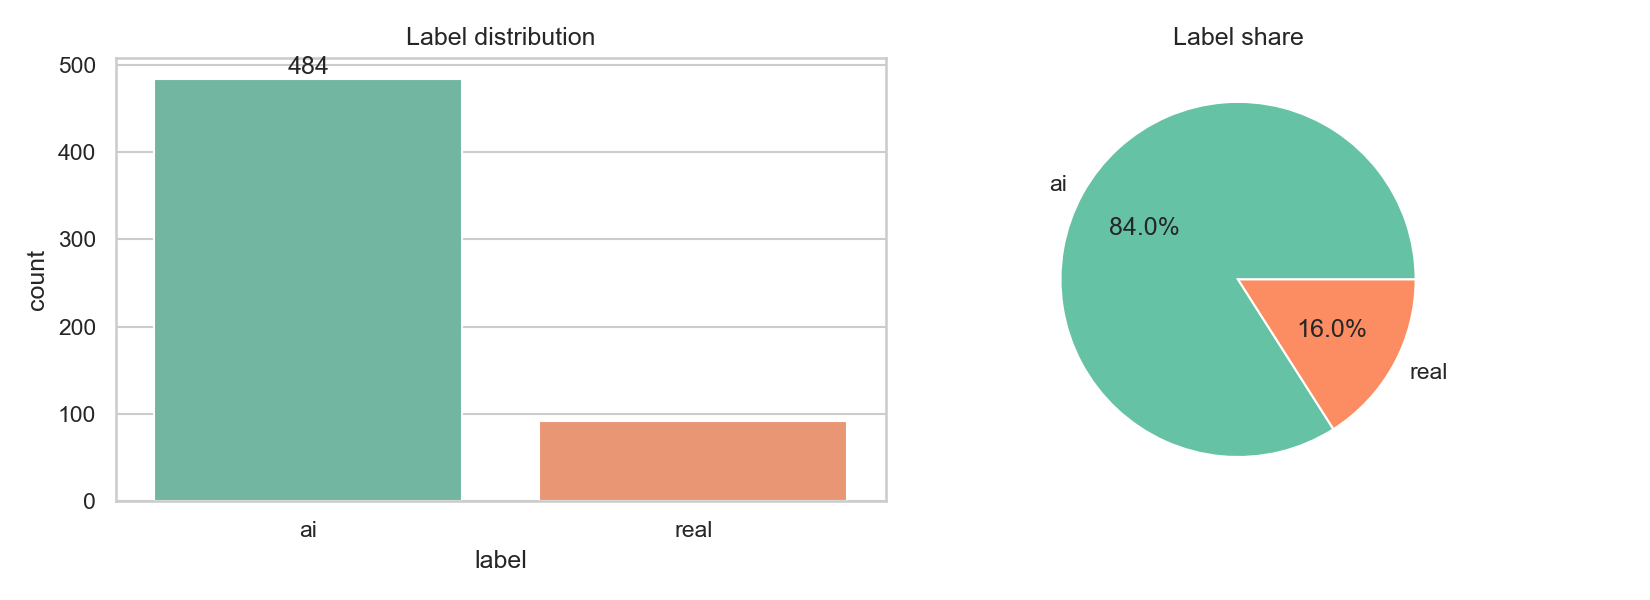
\includegraphics[width=0.75\textwidth]{sonics_label_distribution.png}
  \caption{SONICS label distribution (real vs.\ AI).}
  \label{fig:sonics-label-dist}
\end{figure}

\begin{figure}[H]
  \centering
  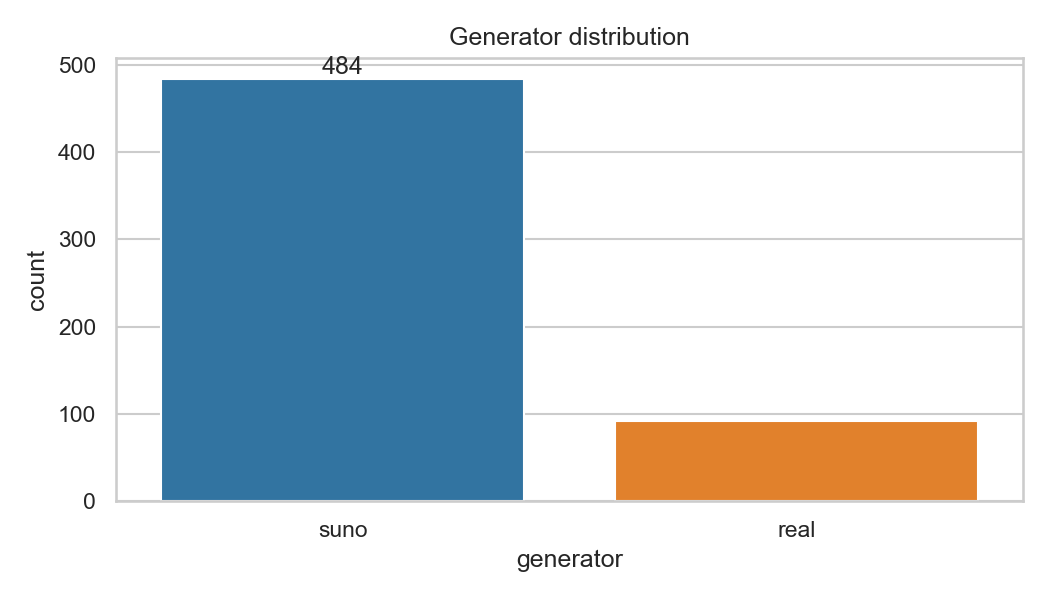
\includegraphics[width=0.70\textwidth]{sonics_generator_distribution.png}
  \caption{SONICS generator distribution (Suno, Udio, human).}
  \label{fig:sonics-gen-dist}
\end{figure}

\begin{figure}[H]
  \centering
  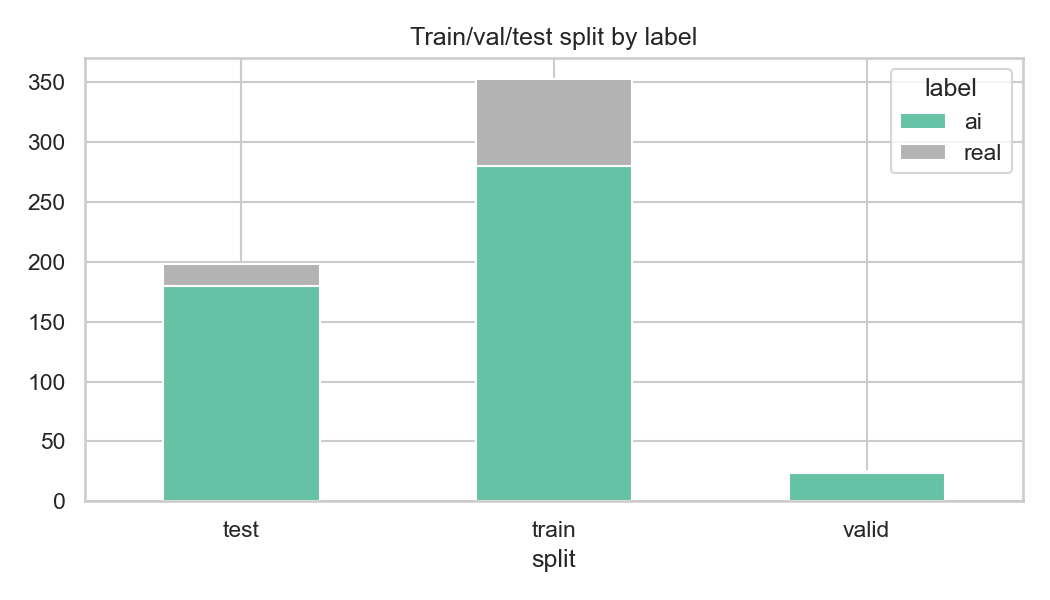
\includegraphics[width=0.70\textwidth]{sonics_split_distribution.png}
  \caption{SONICS train/val/test split by label, confirming stratified partitioning.}
  \label{fig:sonics-split}
\end{figure}

\noindent
Figure~\ref{fig:sonics-spectrograms} shows representative waveforms and mel-spectrograms for one real and one AI-generated track, illustrating the subtle spectral differences that motivate Tier\,2 features.

\begin{figure}[H]
  \centering
  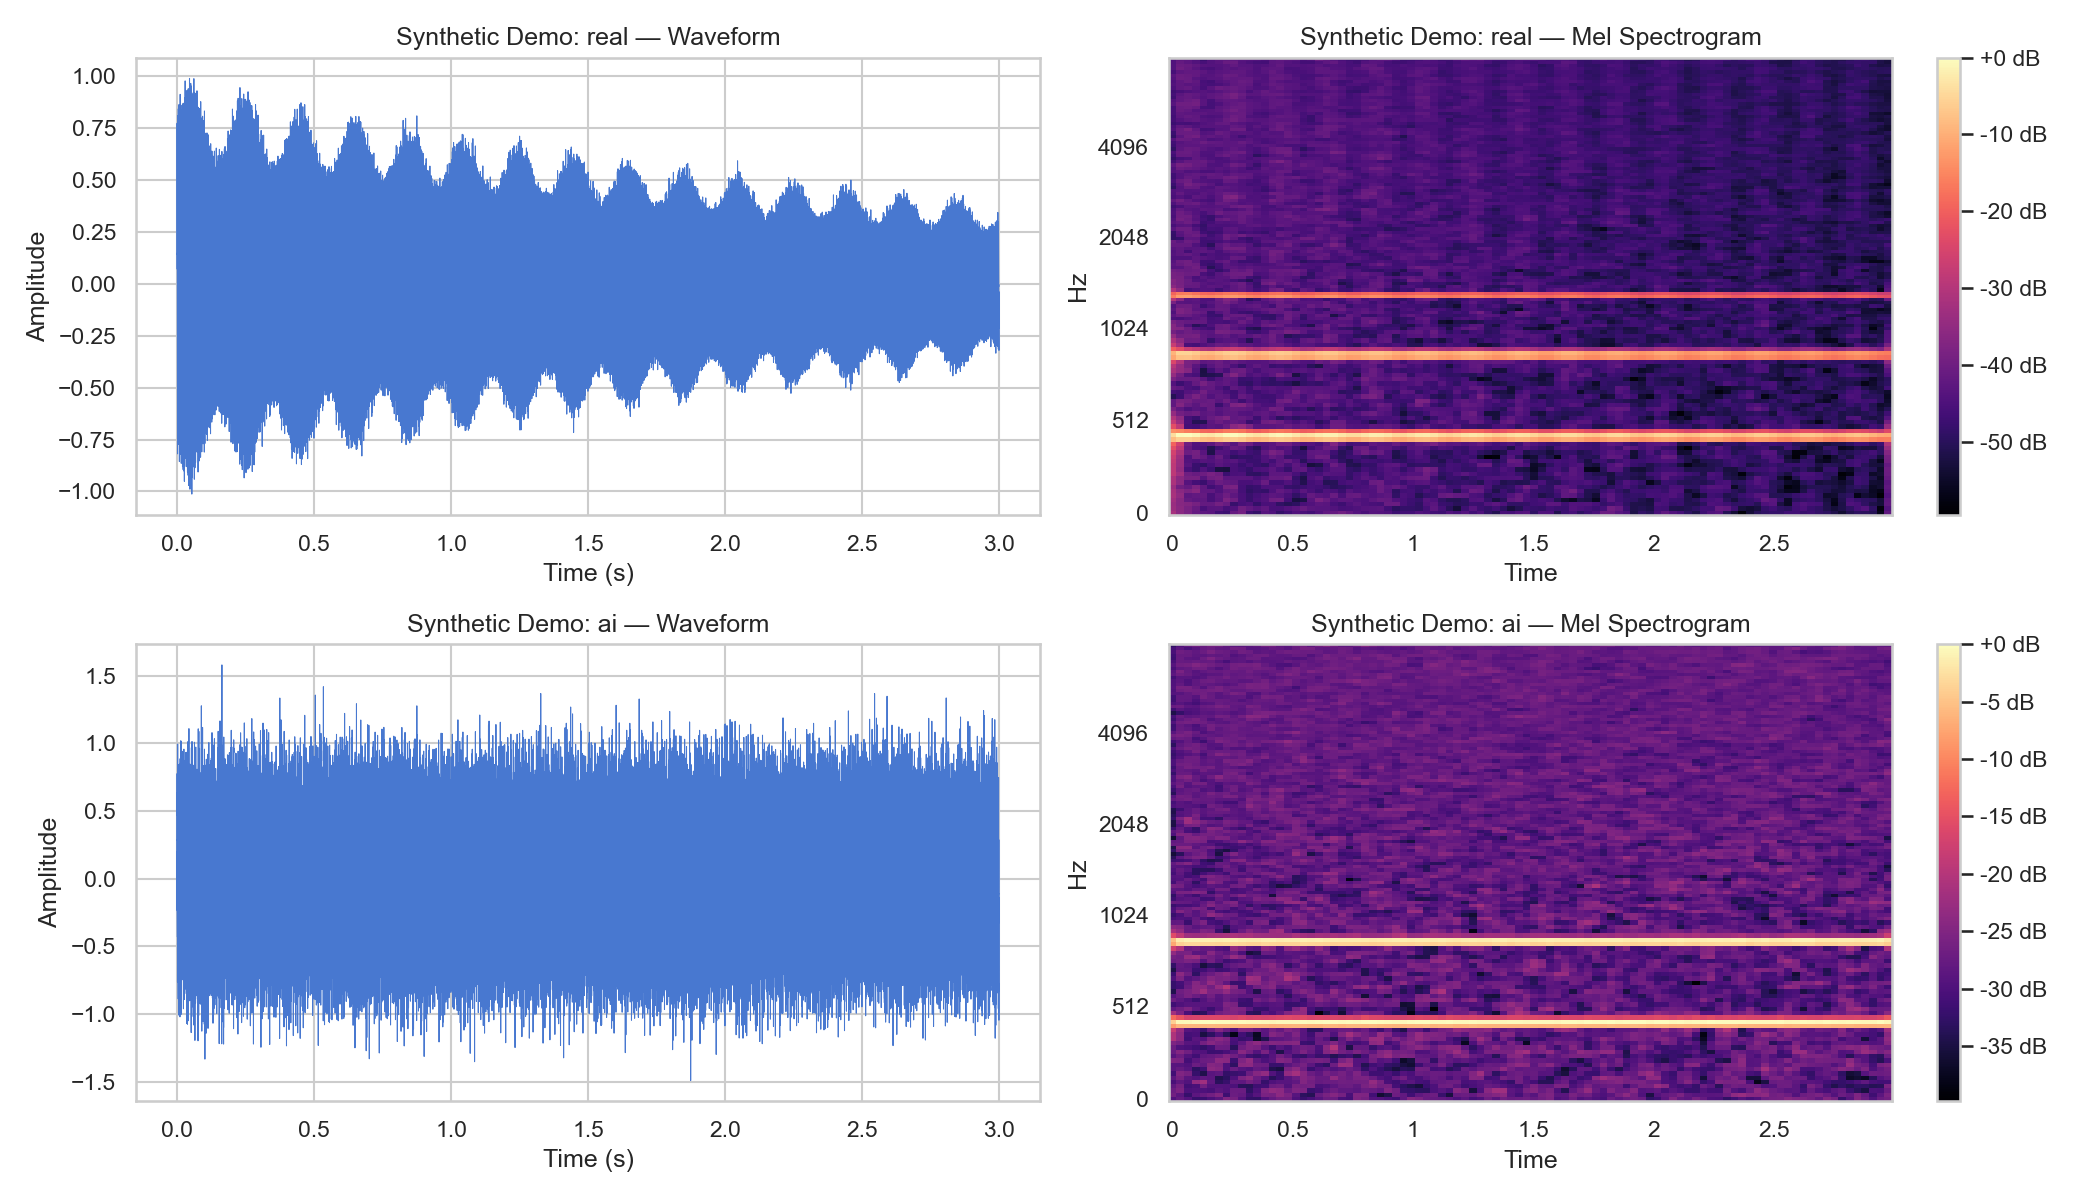
\includegraphics[width=0.95\textwidth]{eda_spectrograms_synthetic_demo.png}
  \caption{Waveforms and mel-spectrograms for a real vs.\ AI-generated track (SONICS, synthetic demo).}
  \label{fig:sonics-spectrograms}
\end{figure}

\begin{figure}[H]
  \centering
  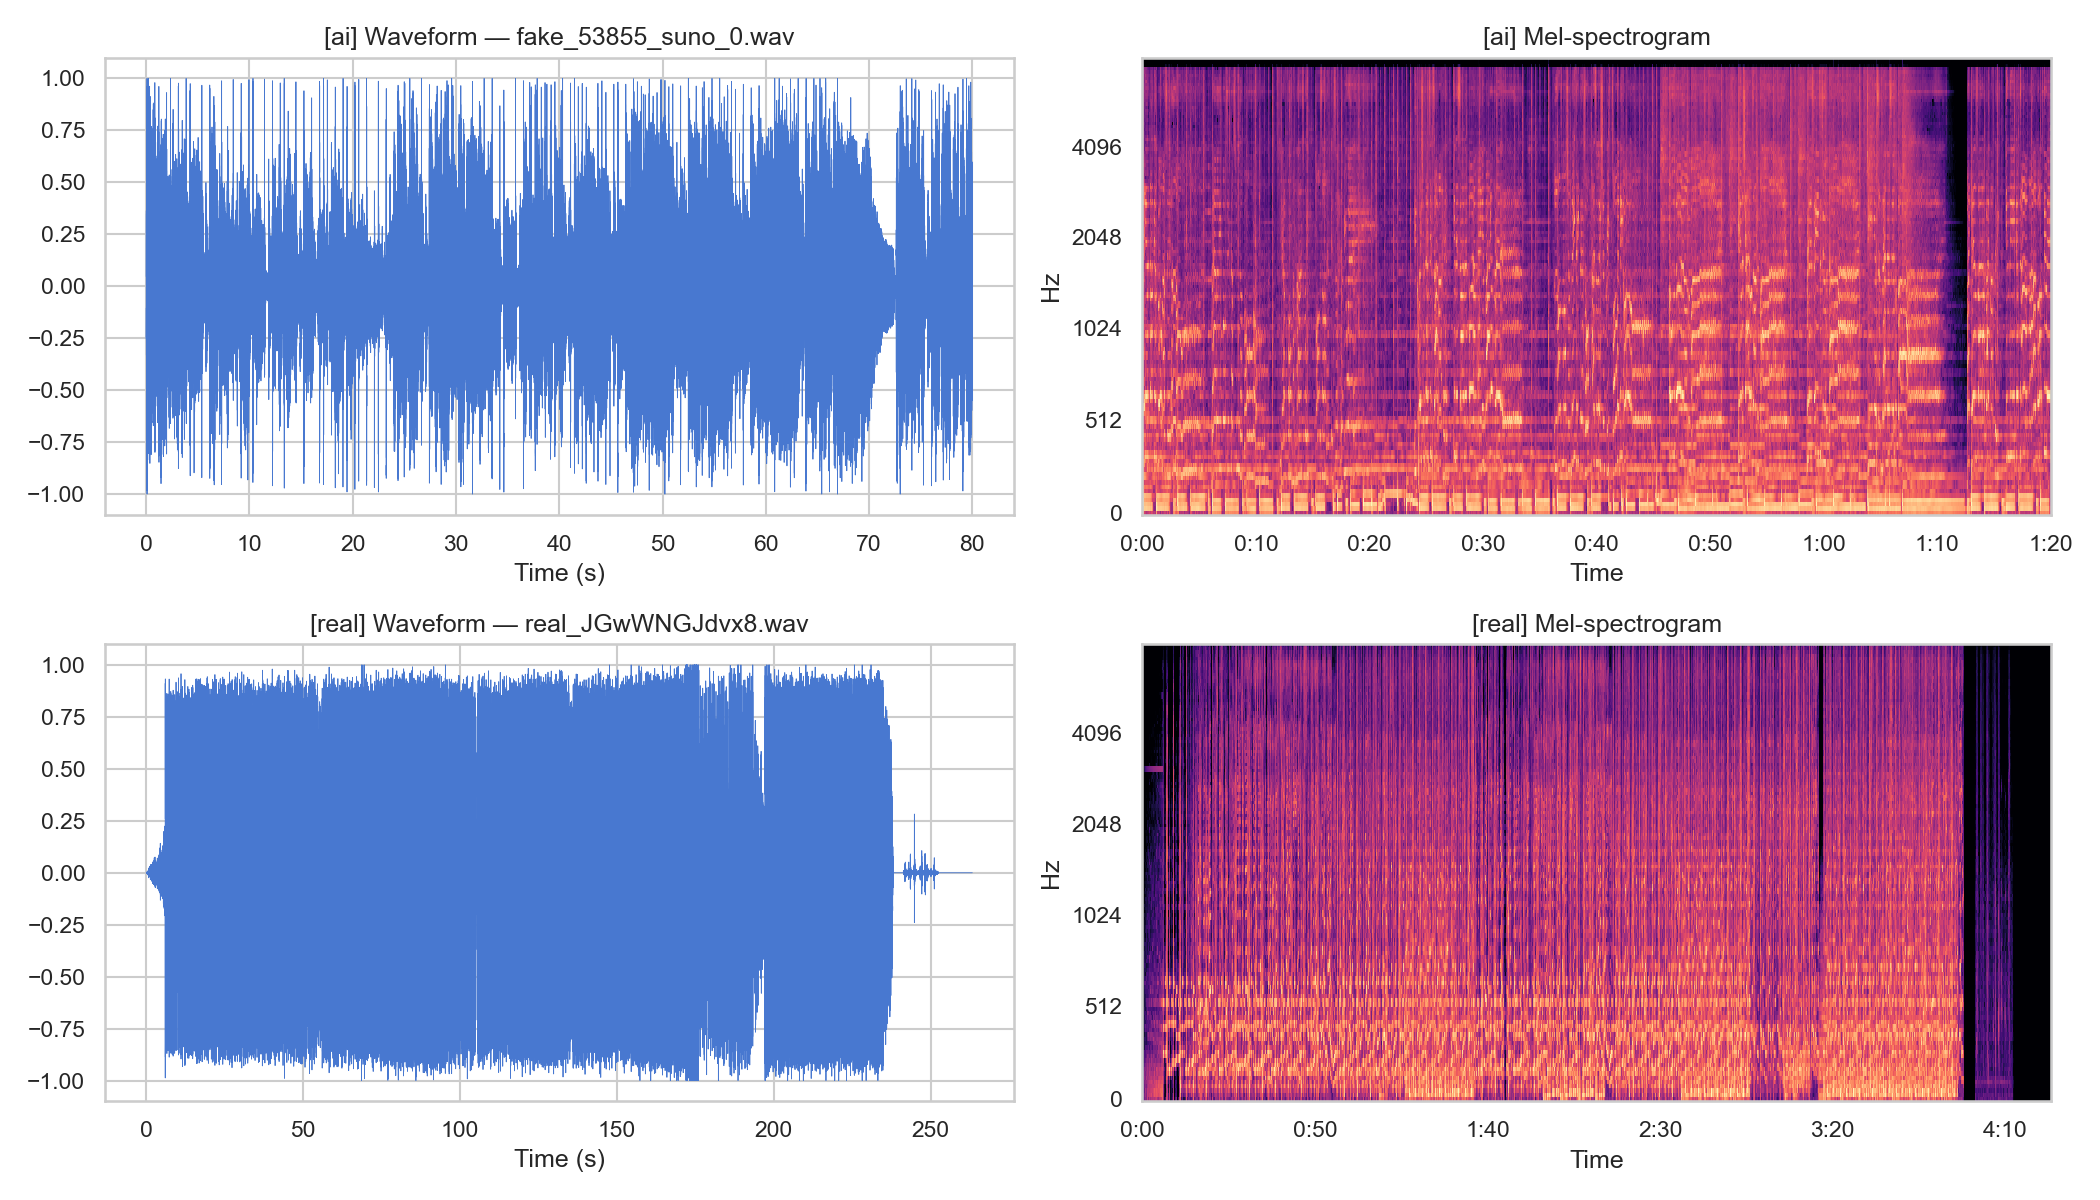
\includegraphics[width=0.95\textwidth]{sonics_spectrograms.png}
  \caption{Waveforms and mel-spectrograms for one track per label (SONICS).}
  \label{fig:sonics-spectrograms-per-label}
\end{figure}

\noindent
Tier\,1 and Tier\,2 feature distributions reveal clear separability between real and AI classes. The top-10 most discriminative Tier\,1 features (ranked by Cohen's $d$) are shown in Figures~\ref{fig:sonics-tier1-box} and~\ref{fig:sonics-tier1-boxplot}.

\begin{figure}[H]
  \centering
  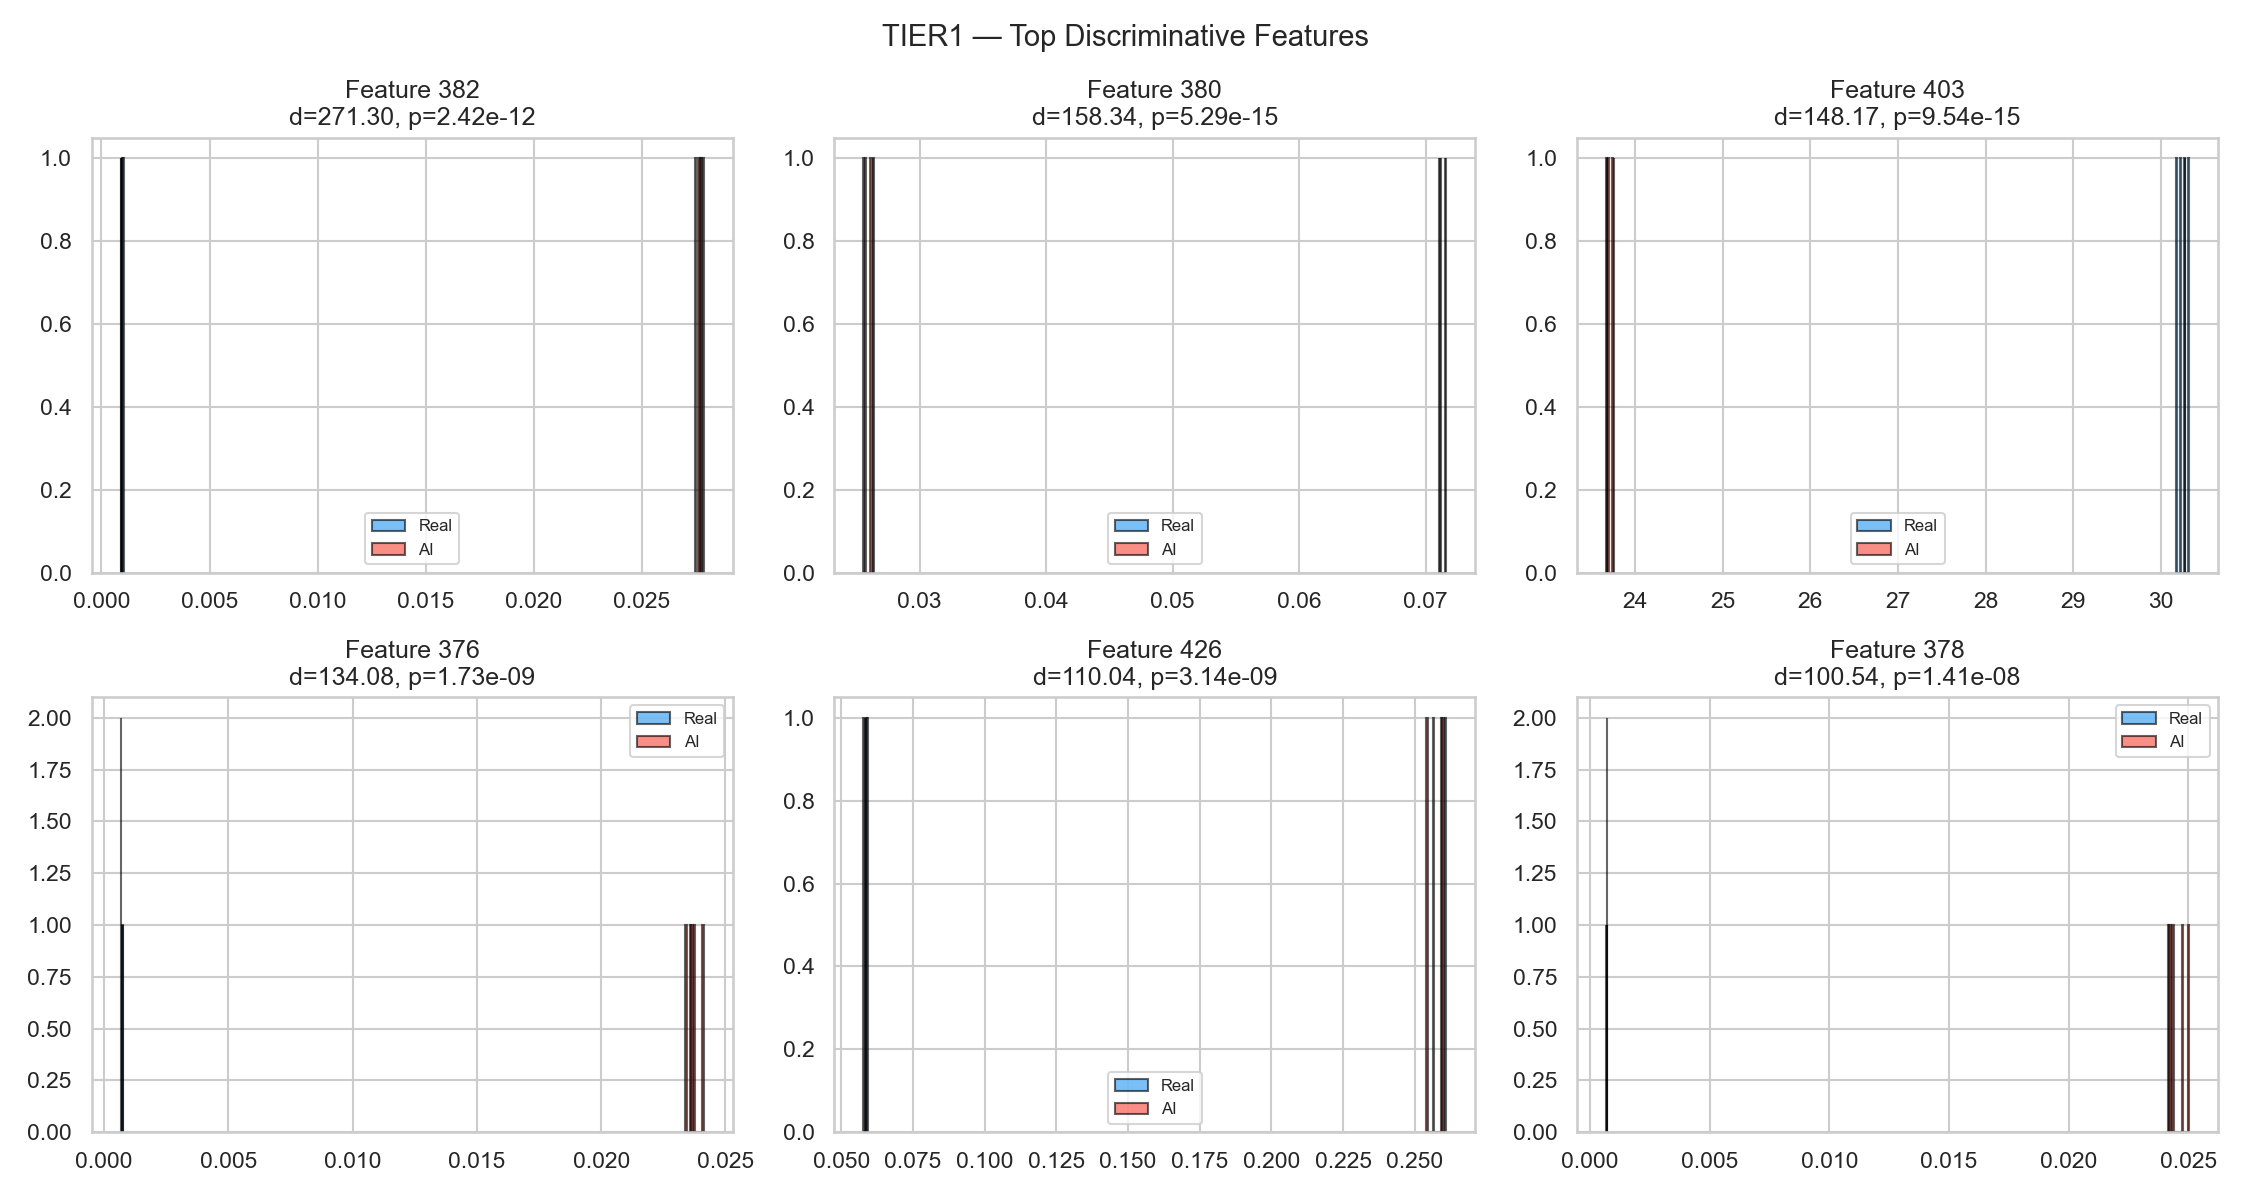
\includegraphics[width=0.95\textwidth]{features_tier1_distributions.png}
  \caption{Tier\,1 feature distributions: real vs.\ AI classes (SONICS).}
  \label{fig:sonics-tier1-box}
\end{figure}

\begin{figure}[H]
  \centering
  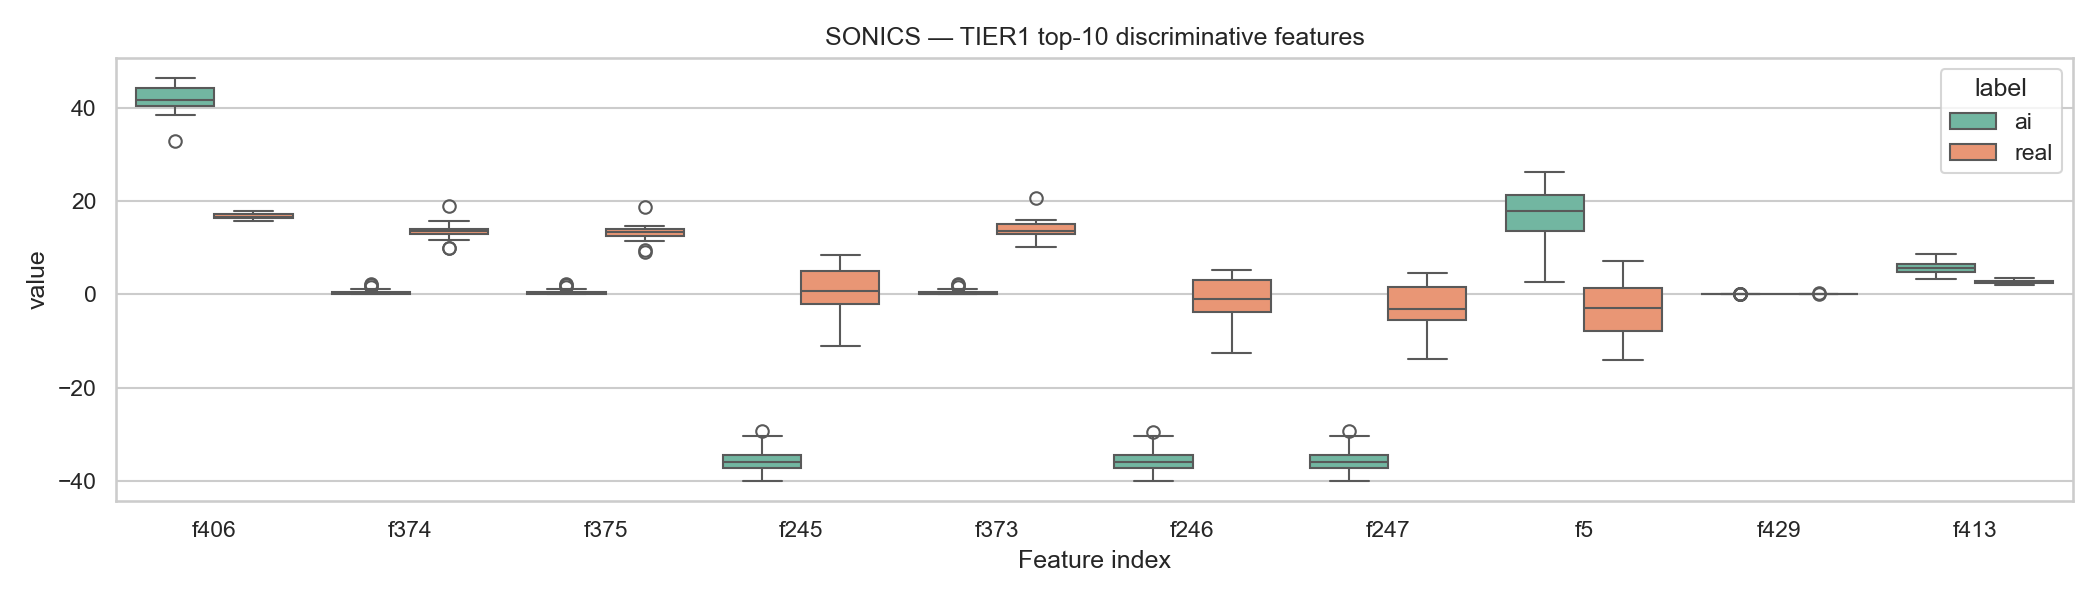
\includegraphics[width=0.95\textwidth]{sonics_tier1_boxplot.png}
  \caption{SONICS Tier\,1 top-10 discriminative features (boxplot by label).}
  \label{fig:sonics-tier1-boxplot}
\end{figure}

\begin{figure}[H]
  \centering
  
\includegraphics[width=0.95\textwidth]{features_tier1_mean_diff.png}
  \caption{Tier\,1 feature mean differences between real and AI classes (SONICS).}
  \label{fig:tier1-mean-diff}
\end{figure}

\begin{figure}[H]
  \centering
  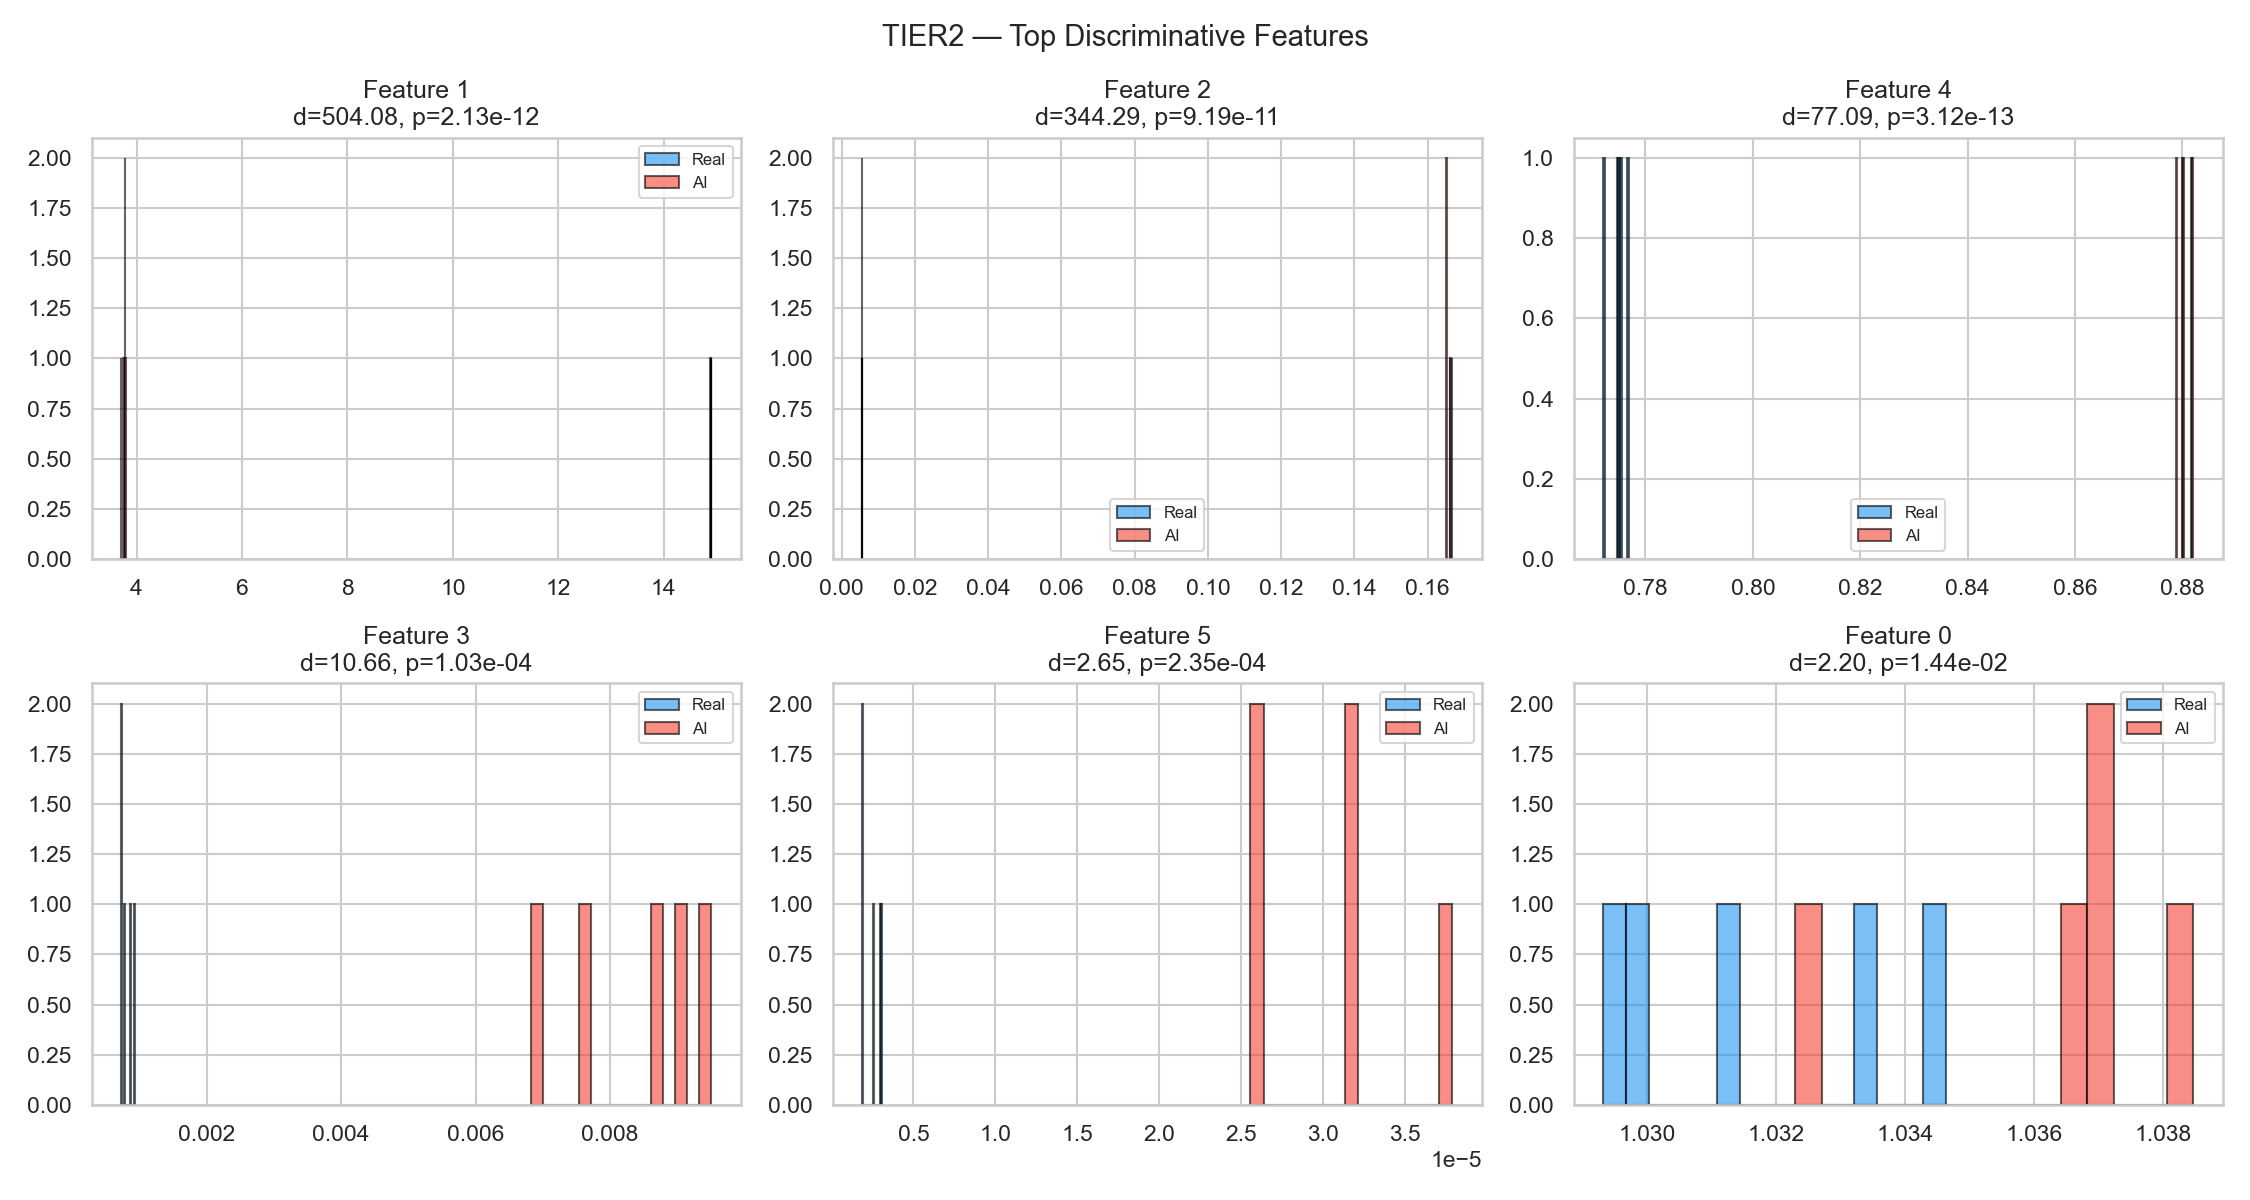
\includegraphics[width=0.95\textwidth]{features_tier2_distributions.png}
  \caption{Tier\,2 AI-artifact feature distributions: real vs.\ AI classes (SONICS).}
  \label{fig:sonics-tier2-box}
\end{figure}

\begin{figure}[H]
  \centering
  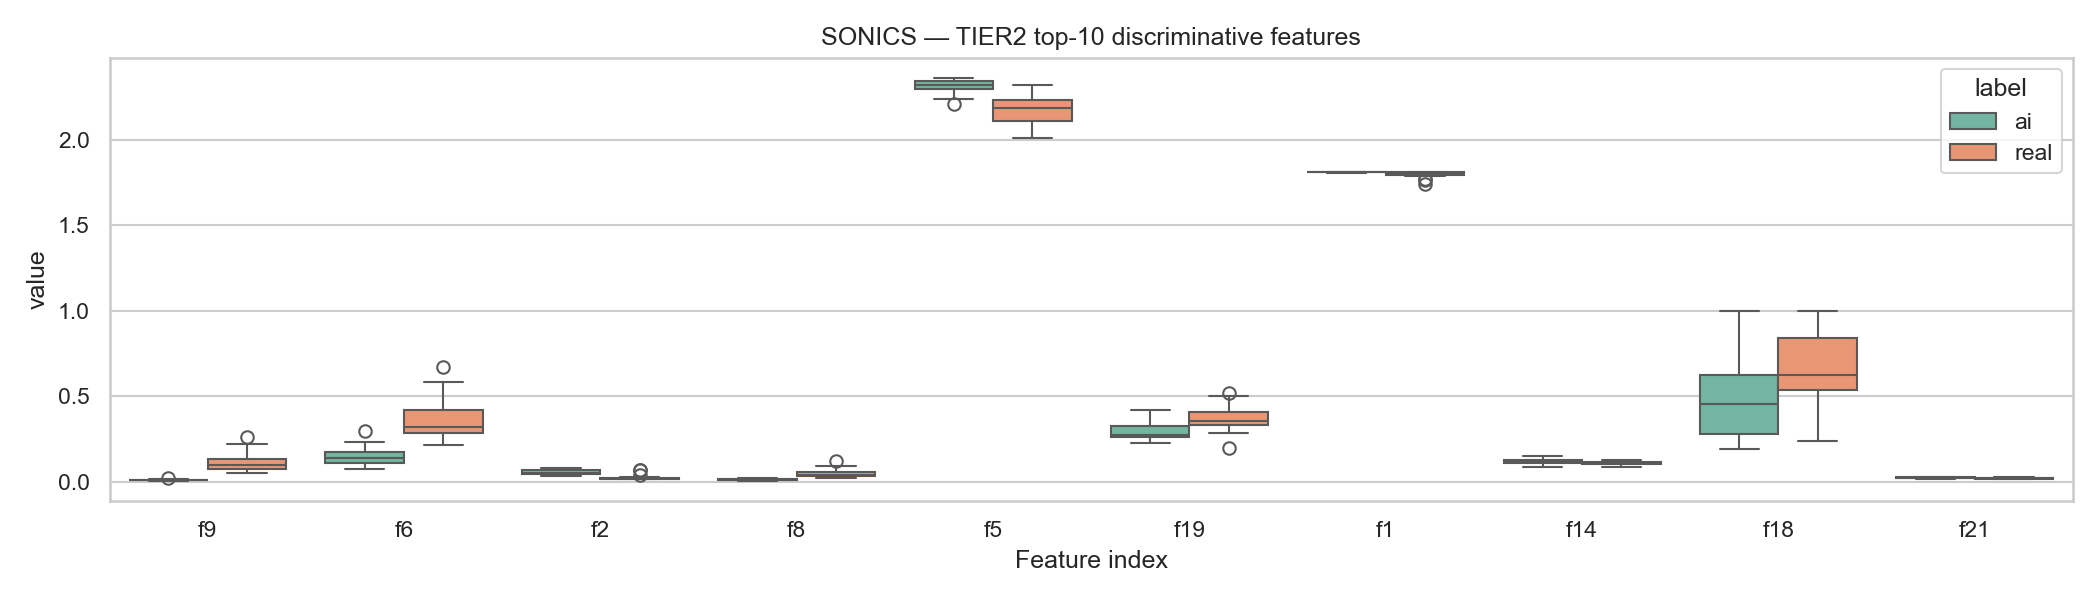
\includegraphics[width=0.95\textwidth]{sonics_tier2_boxplot.png}
  \caption{SONICS Tier\,2 top-10 discriminative features (boxplot by label).}
  \label{fig:sonics-tier2-boxplot}
\end{figure}

\begin{figure}[H]
  \centering
  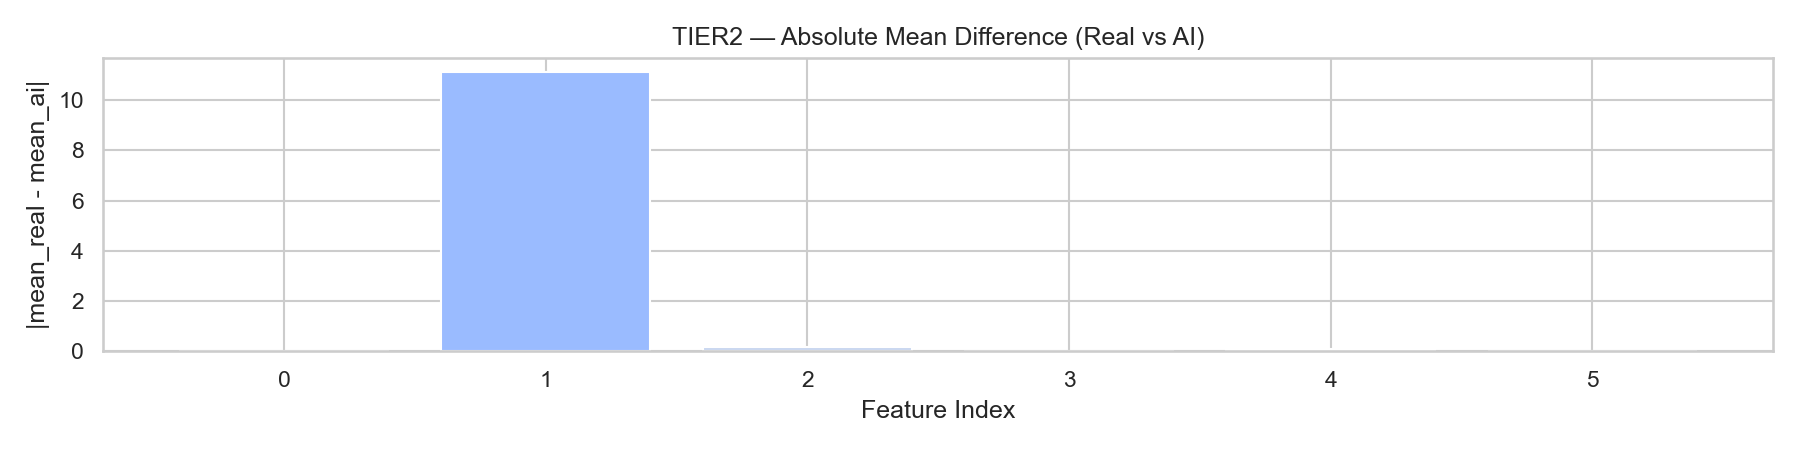
\includegraphics[width=0.95\textwidth]{features_tier2_mean_diff.png}
  \caption{Tier\,2 feature mean differences between real and AI classes (SONICS).}
  \label{fig:tier2-mean-diff}
\end{figure}

\begin{figure}[H]
  \centering
  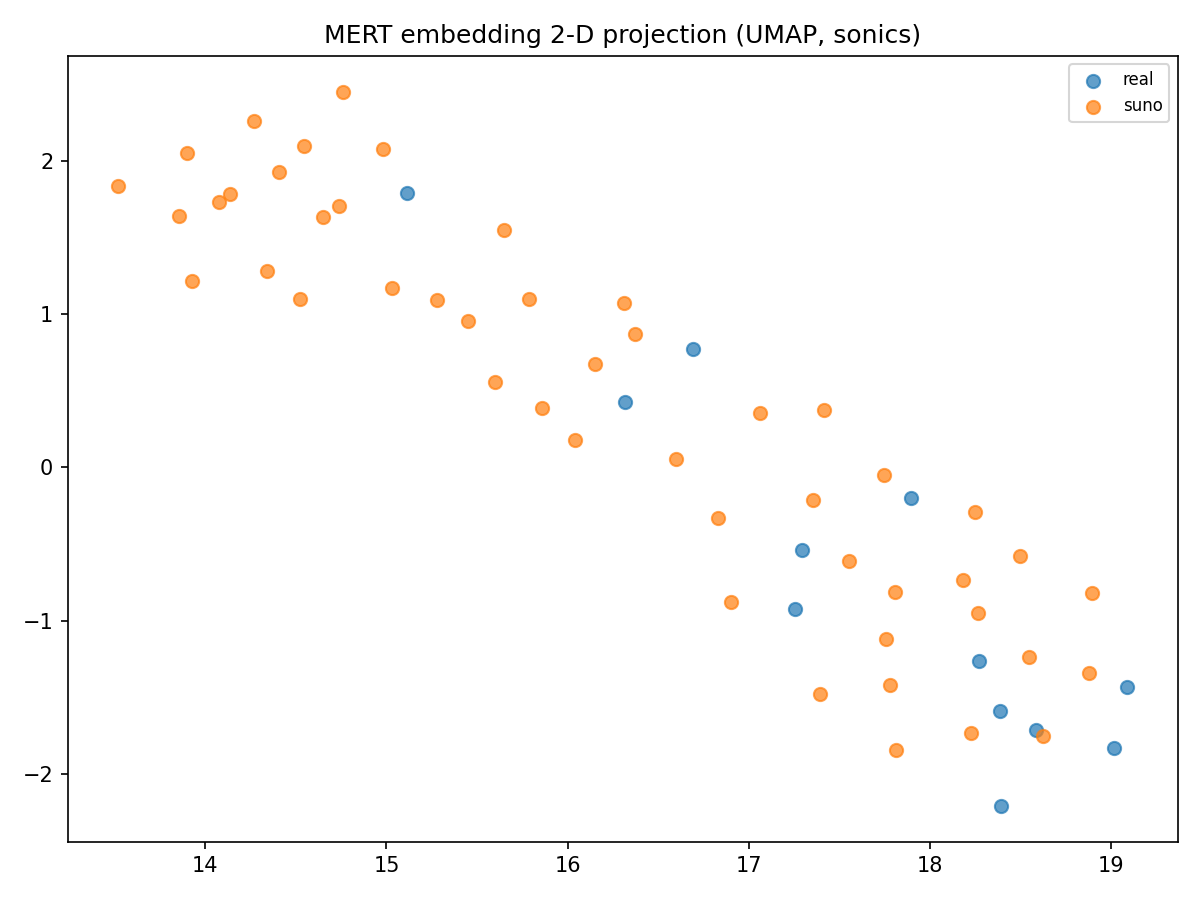
\includegraphics[width=0.85\textwidth]{sonics_mert_projection.png}
  \caption{MERT embedding 2-D projection (UMAP/t-SNE) coloured by label and generator (SONICS). Clear cluster separation validates MERT as a discriminative backbone.}
  \label{fig:sonics-mert}
\end{figure}

\begin{figure}[H]
  \centering
  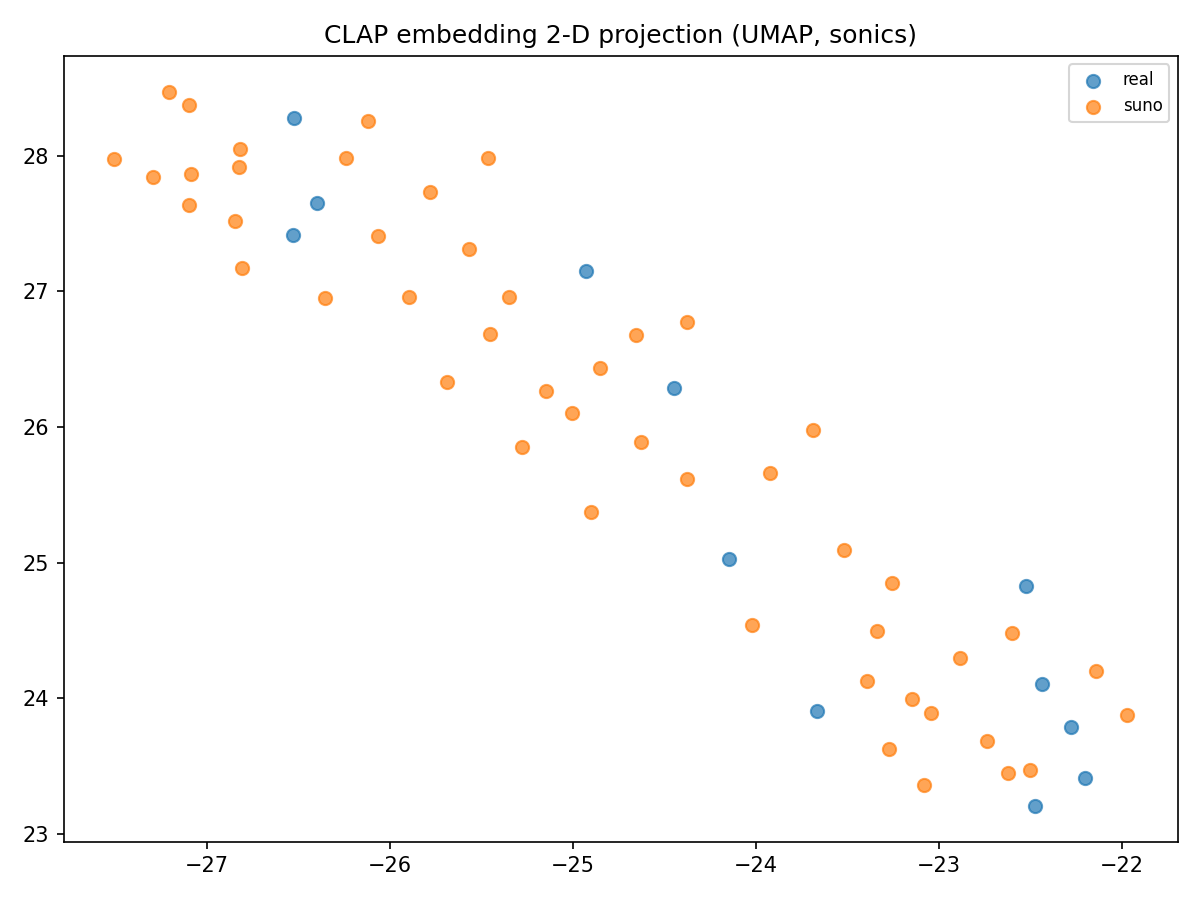
\includegraphics[width=0.85\textwidth]{sonics_clap_projection.png}
  \caption{CLAP embedding 2-D projection coloured by label and generator (SONICS). Compared with the MERT projection (Figure~\ref{fig:sonics-mert}), the CLAP space shows a different cluster geometry, confirming that fusing both embedding families captures complementary structure.}
  \label{fig:sonics-clap}
\end{figure}

\begin{figure}[H]
  \centering
  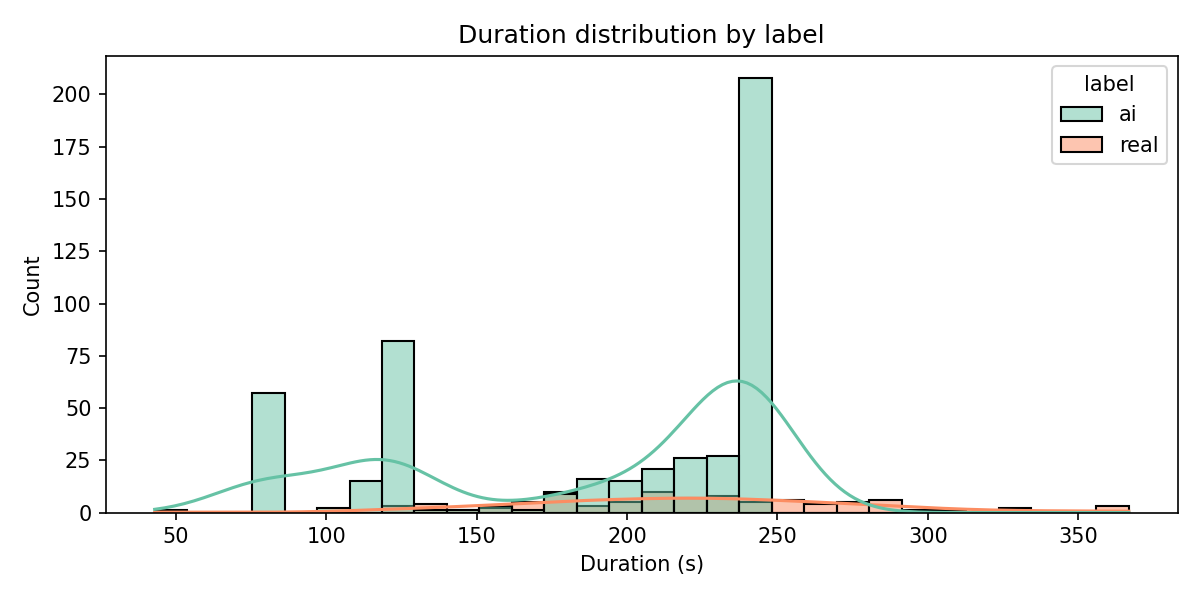
\includegraphics[width=0.75\textwidth]{sonics_duration_distribution.png}
  \caption{Track duration distribution by label (SONICS). Most tracks cluster around 10\,s, validating the fixed-length chunking window used in the pipeline.}
  \label{fig:sonics-duration}
\end{figure}

\noindent
\textbf{Insight:} Tier\,2 features (phase continuity, HNR, Fourier artifact energy) show stronger class separation than many Tier\,1 features (compare Figures~\ref{fig:sonics-tier1-boxplot} and~\ref{fig:sonics-tier2-boxplot}), confirming that AI generators leave detectable spectral fingerprints. The mean-difference plots (Figures~\ref{fig:tier1-mean-diff} and~\ref{fig:tier2-mean-diff}) highlight which specific dimensions drive the separation. However, Tier\,1 features capture complementary timbral variation (MFCC statistics, mel-spectrogram shape) that improves overall discriminability when combined. The MERT embedding projection (Figure~\ref{fig:sonics-mert}) shows that deep learned representations achieve clear cluster separation between real and AI-generated tracks even in two dimensions, while the CLAP projection (Figure~\ref{fig:sonics-clap}) reveals complementary structure that motivates multi-modal fusion. The duration distribution (Figure~\ref{fig:sonics-duration}) confirms that tracking durations are consistent across labels.


\subsection{FakeMusicCaps}

FakeMusicCaps pairs text captions from the original MusicCaps dataset with AI-generated audio from five different generative models, providing model-level granularity.

\begin{figure}[H]
  \centering
  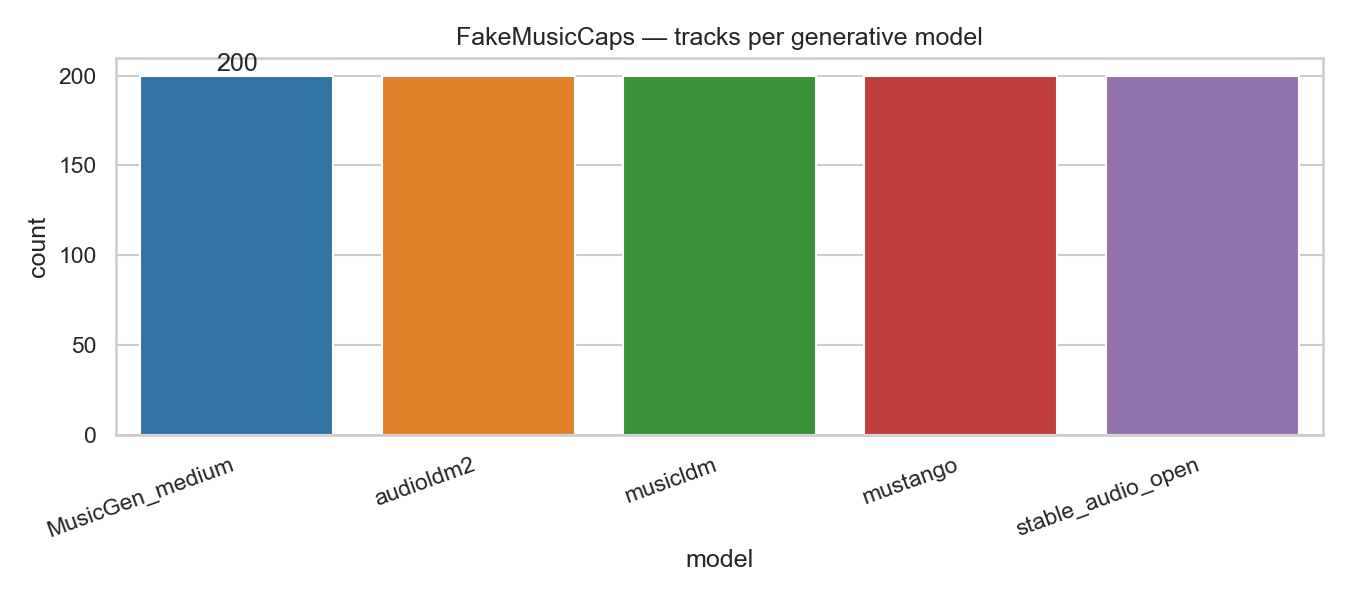
\includegraphics[width=0.85\textwidth]{fakemusiccaps_model_distribution.png}
  \caption{FakeMusicCaps track counts per generative model.}
  \label{fig:fmc-model-dist}
\end{figure}

\begin{itemize}[nosep]
  \item Five generators are represented, enabling per-model analysis of artifact signatures.
  \item Captions provide text grounding; caption length clusters around 10--20 words (Figure~\ref{fig:fmc-captions}).
  \item Tier\,1 feature heatmaps (Figure~\ref{fig:fmc-heatmap}) reveal that different generators produce distinct spectral profiles, with MusicGen and Riffusion occupying separate regions of feature space.
\end{itemize}

\begin{figure}[H]
  \centering
  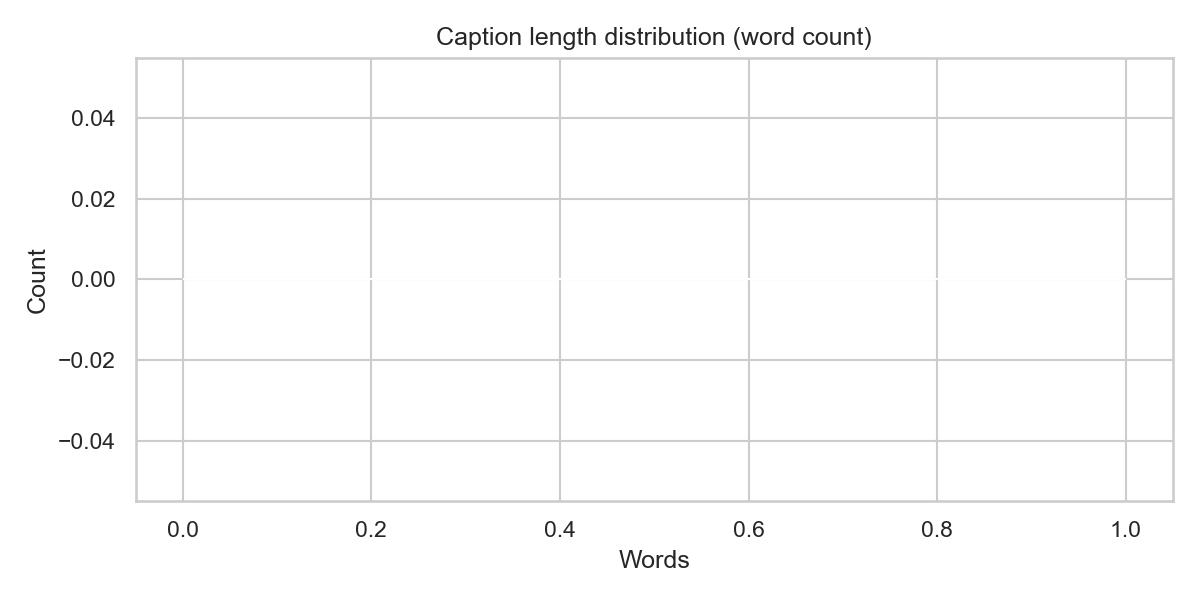
\includegraphics[width=0.85\textwidth]{fakemusiccaps_caption_lengths.png}
  \caption{Caption length (word count) distribution in FakeMusicCaps.}
  \label{fig:fmc-captions}
\end{figure}

\begin{figure}[H]
  \centering
  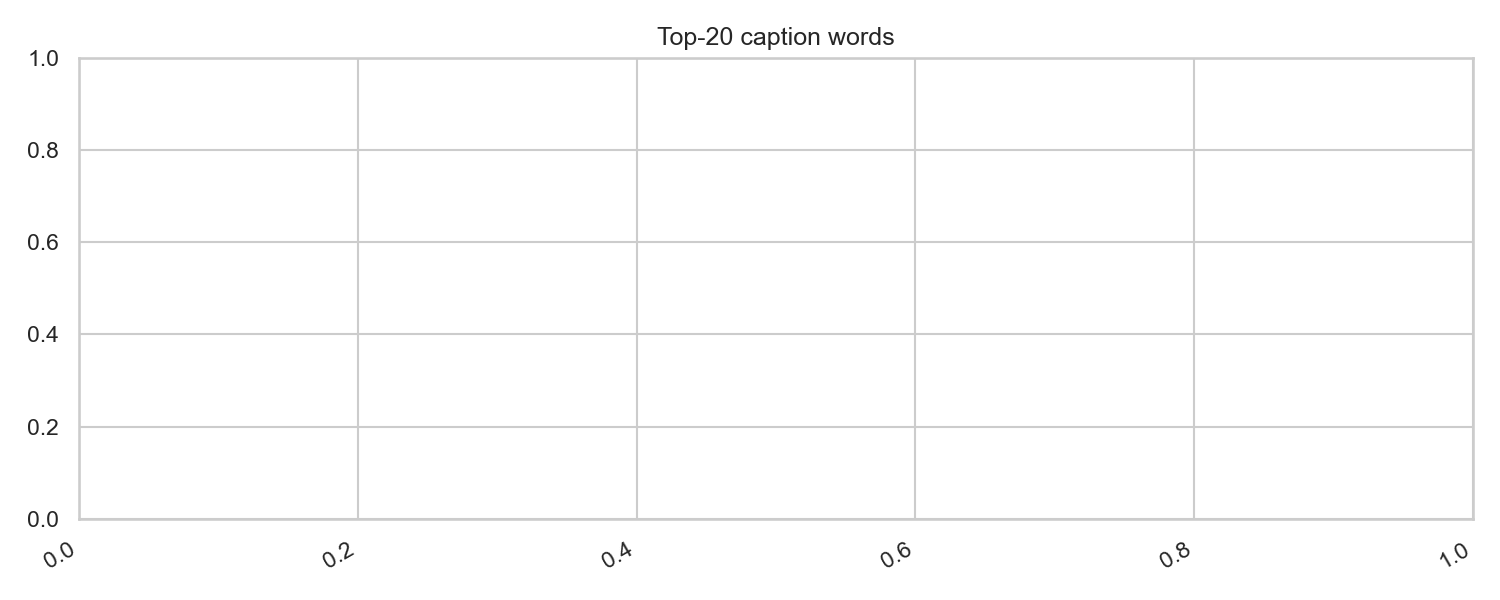
\includegraphics[width=0.95\textwidth]{fakemusiccaps_caption_words.png}
  \caption{Top-20 most frequent caption words in FakeMusicCaps (stopwords excluded). Dominant terms (``piano'', ``guitar'', ``melody'') reflect the genre composition of the dataset.}
  \label{fig:fmc-caption-words}
\end{figure}

\begin{figure}[H]
  \centering
  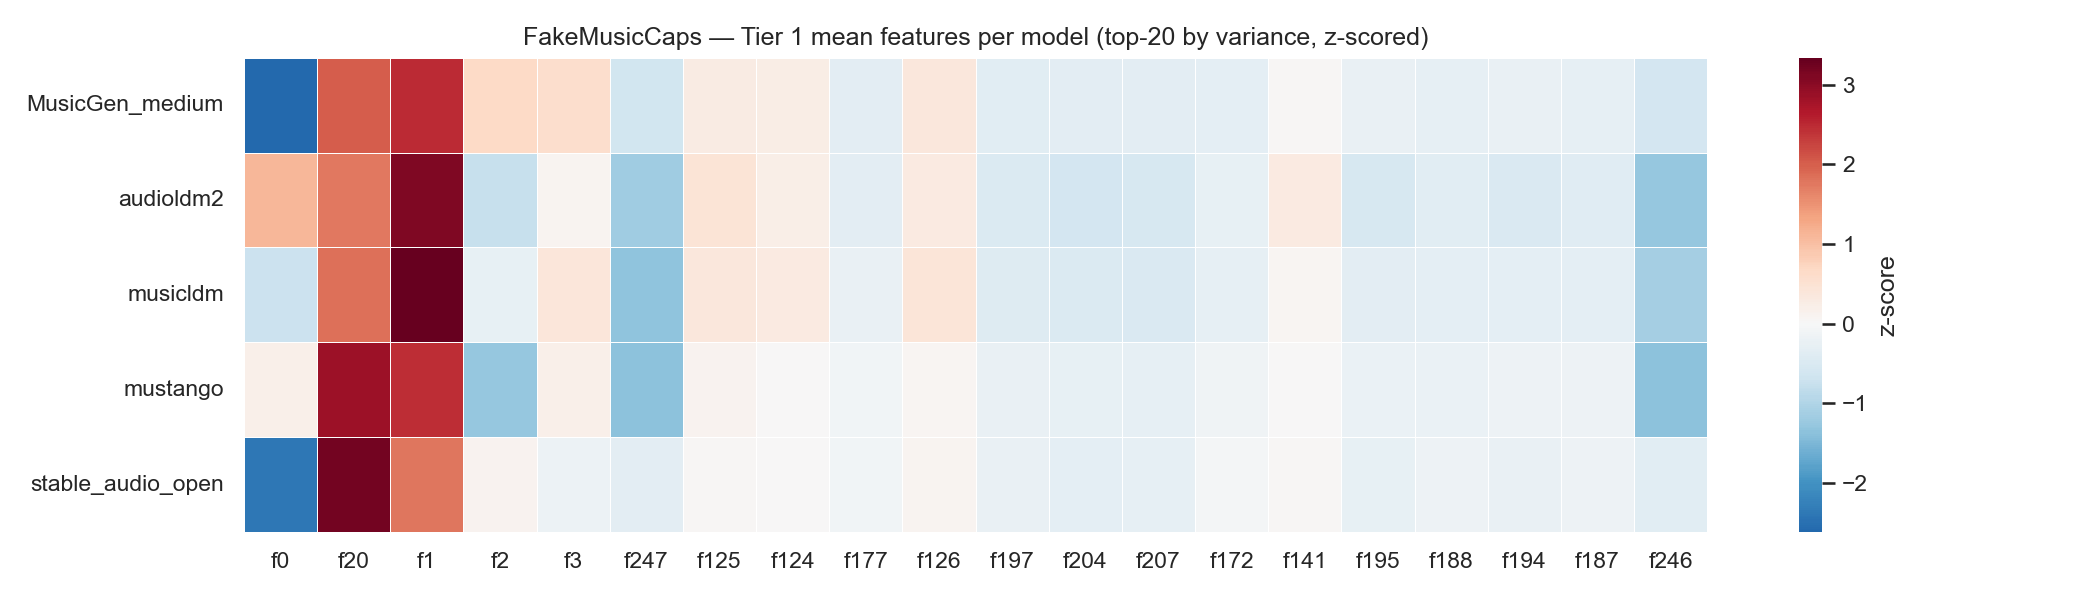
\includegraphics[width=0.95\textwidth]{fakemusiccaps_tier1_heatmap.png}
  \caption{Tier\,1 mean feature heatmap per generator (top-20 dims by inter-model variance, z-scored). Different generators occupy distinct spectral profiles.}
  \label{fig:fmc-heatmap}
\end{figure}

\begin{figure}[H]
  \centering
  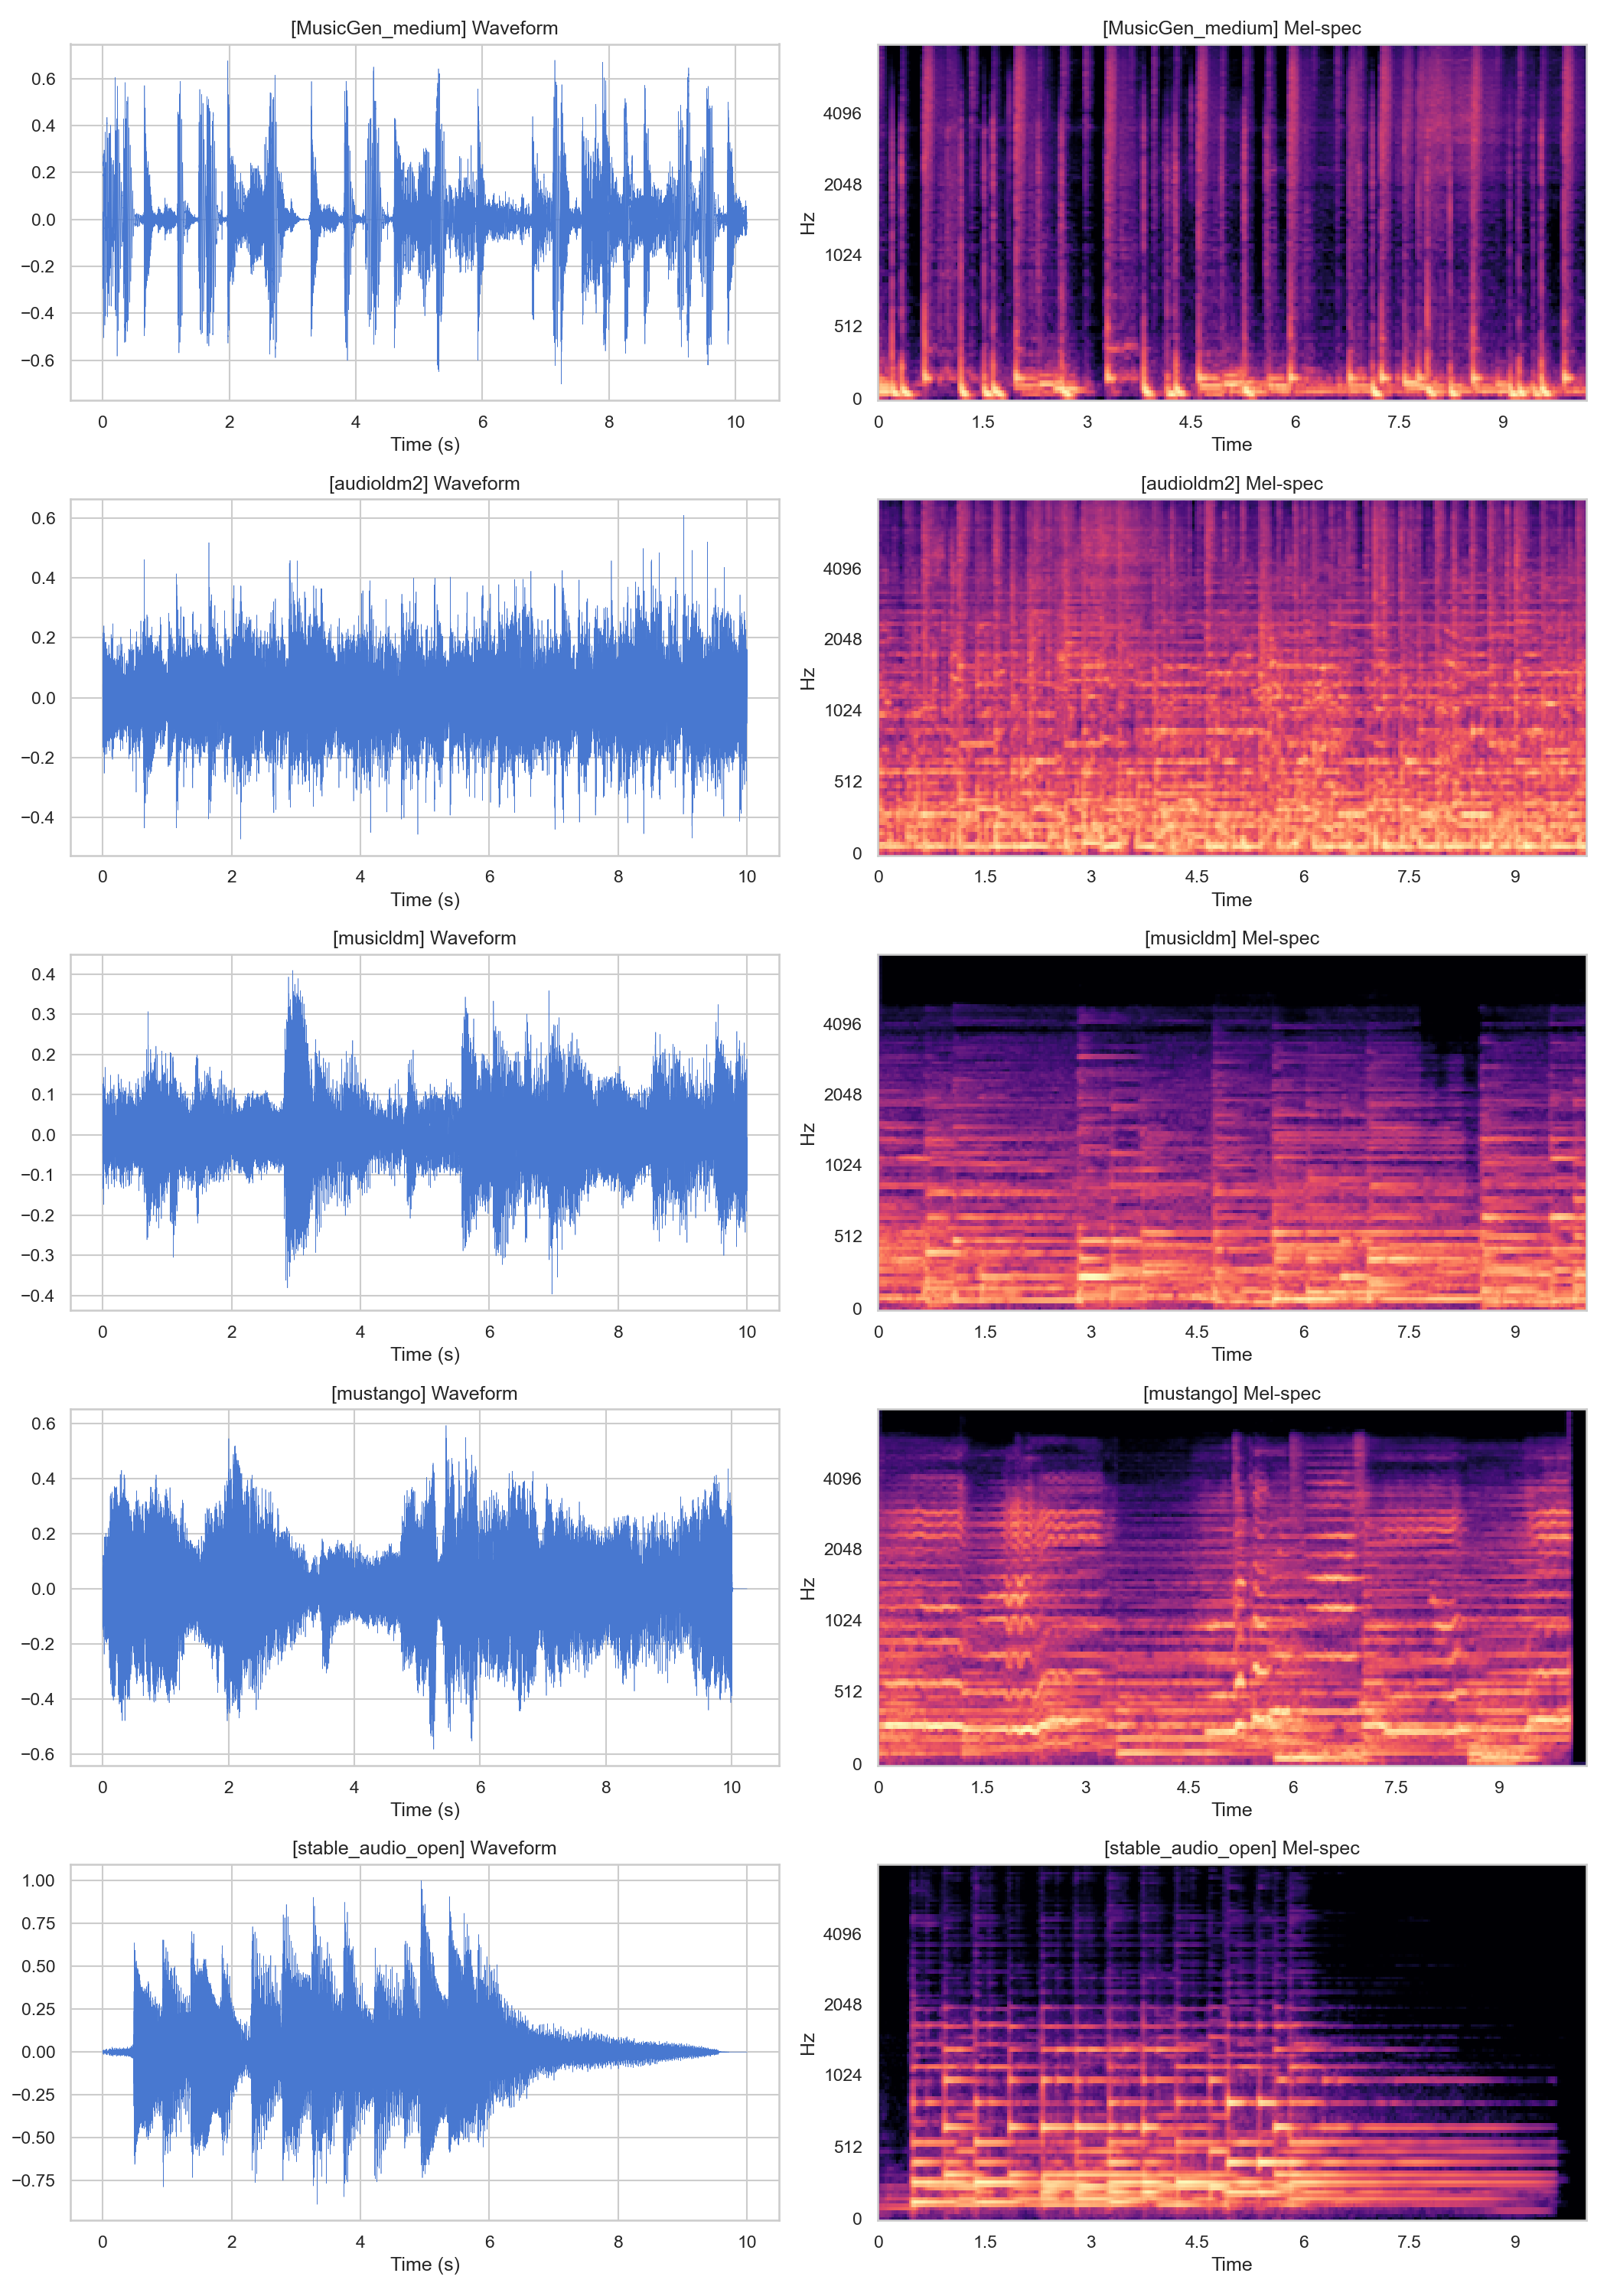
\includegraphics[width=0.95\textwidth]{fakemusiccaps_spectrograms.png}
  \caption{Waveforms and mel-spectrograms for one track per generator (FakeMusicCaps).}
  \label{fig:fmc-spectrograms}
\end{figure}

\begin{figure}[H]
  \centering
  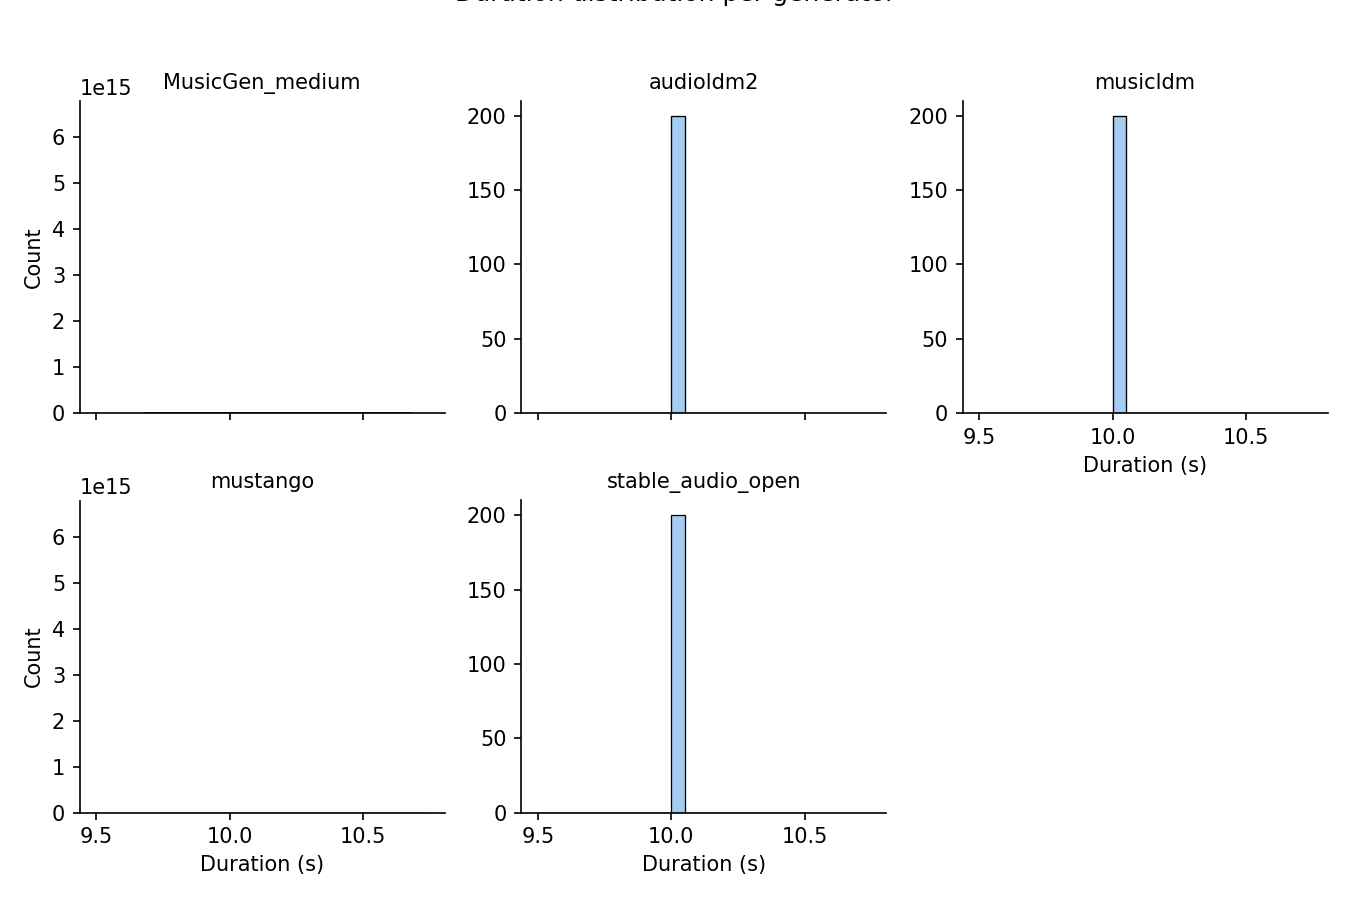
\includegraphics[width=0.85\textwidth]{fakemusiccaps_duration_by_model.png}
  \caption{Track duration distributions faceted by generative model (FakeMusicCaps). Duration variability differs across generators, with some producing fixed-length outputs.}
  \label{fig:fmc-duration}
\end{figure}

\begin{figure}[H]
  \centering
  \begin{subfigure}[b]{0.48\textwidth}
    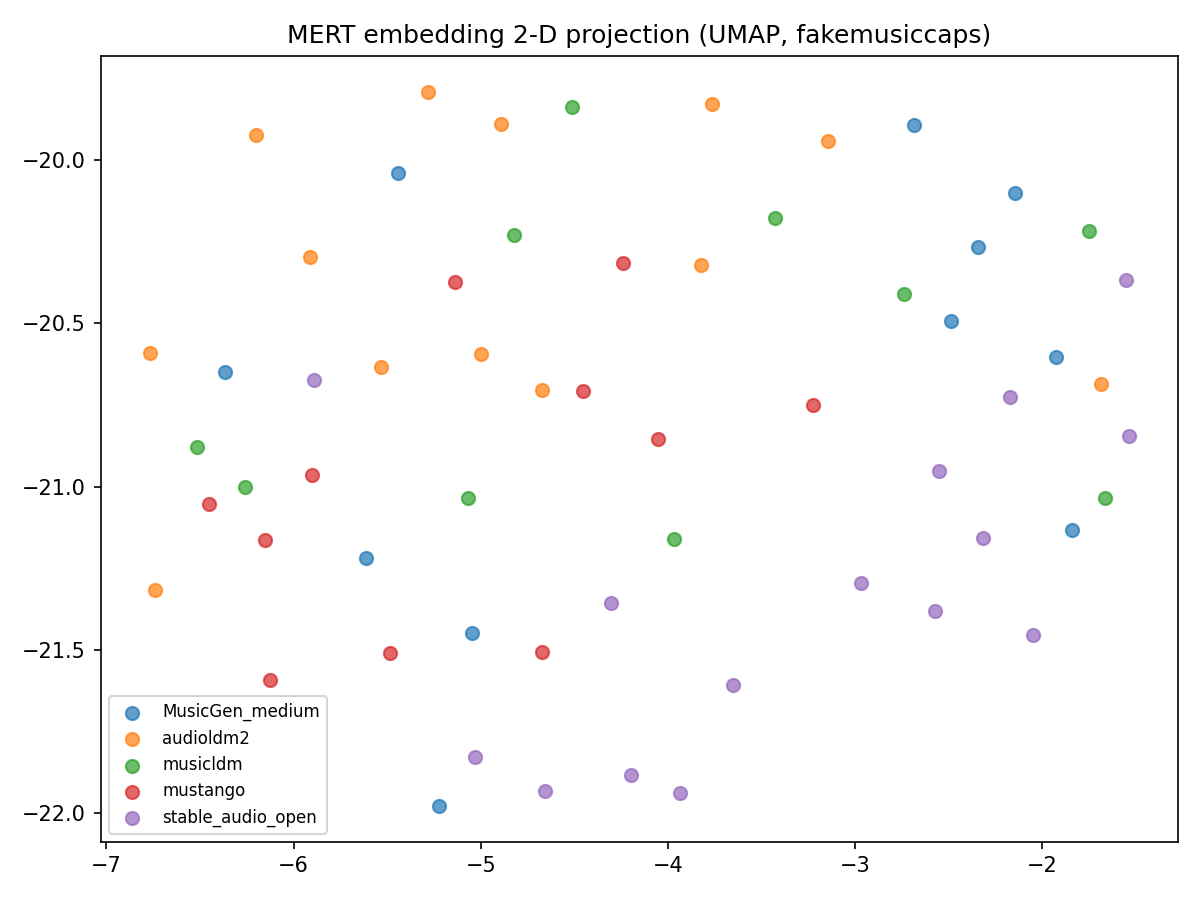
\includegraphics[width=\textwidth]{fakemusiccaps_mert_projection.png}
    \caption{MERT embedding projection.}
    \label{fig:fmc-mert}
  \end{subfigure}
  \hfill
  \begin{subfigure}[b]{0.48\textwidth}
    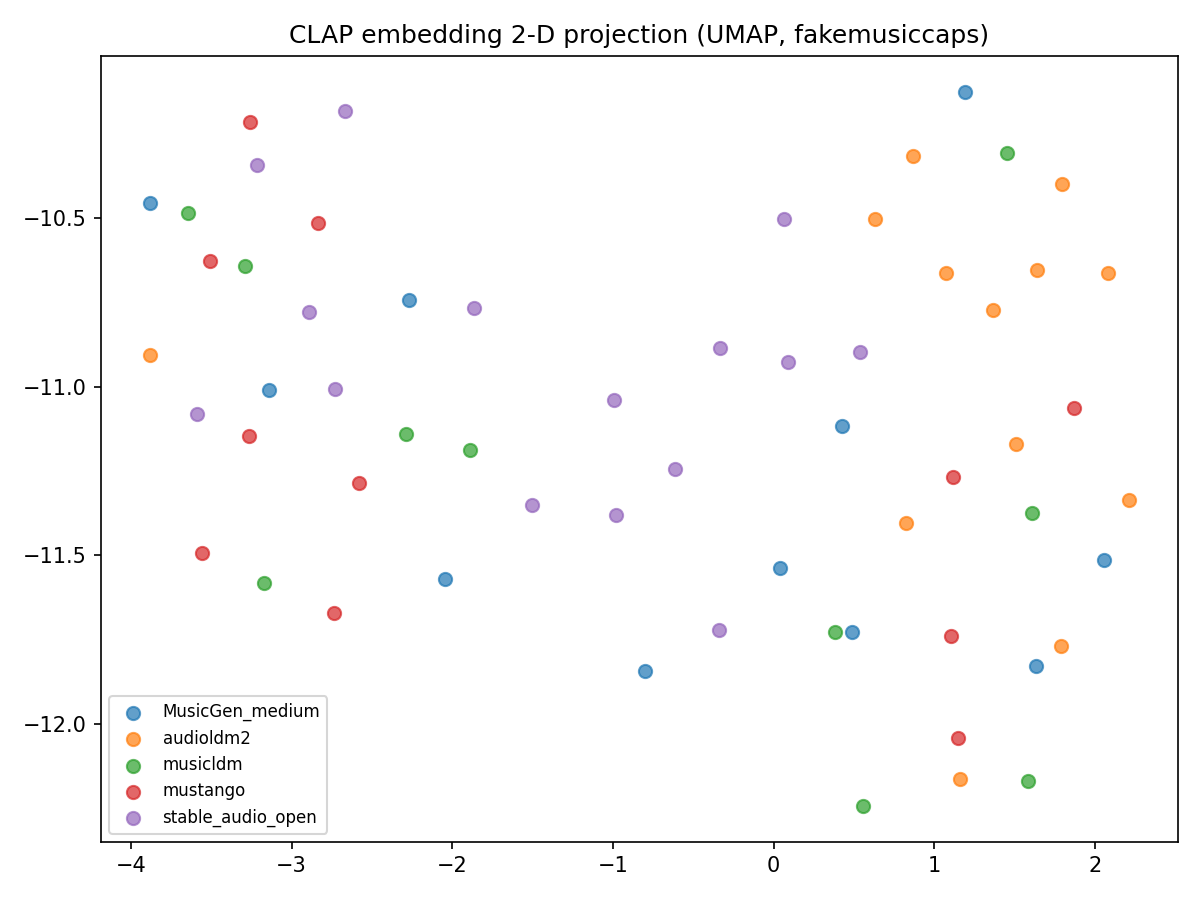
\includegraphics[width=\textwidth]{fakemusiccaps_clap_projection.png}
    \caption{CLAP embedding projection.}
    \label{fig:fmc-clap}
  \end{subfigure}
  \caption{2-D embedding projections coloured by generator (FakeMusicCaps). Each model occupies a distinct region, particularly in the MERT space.}
  \label{fig:fmc-projections}
\end{figure}

\noindent
\textbf{Insight:} The inter-model variance in Tier\,1 features confirms that a single ``AI'' class is an oversimplification; each generator family leaves a different spectral signature. The MERT and CLAP projections (Figure~\ref{fig:fmc-projections}) show that generators form distinct clusters, with MERT providing tighter separation. Duration facets (Figure~\ref{fig:fmc-duration}) reveal that some generators produce fixed-length outputs, which is itself a detectable artifact. This motivates the multi-tier feature design and explains why a learned neural similarity head outperforms any single handcrafted threshold.


\subsection{MIPPIA (Music Plagiarism Dataset)}

MIPPIA provides 70 song pairs labelled as plagiarism (\texttt{plag}), doubtful plagiarism (\texttt{plag\_doubt}), or remake (\texttt{remake}), with segment-level similarity timestamps. It is the only dataset with genuine pairwise structure.

\begin{figure}[H]
  \centering
  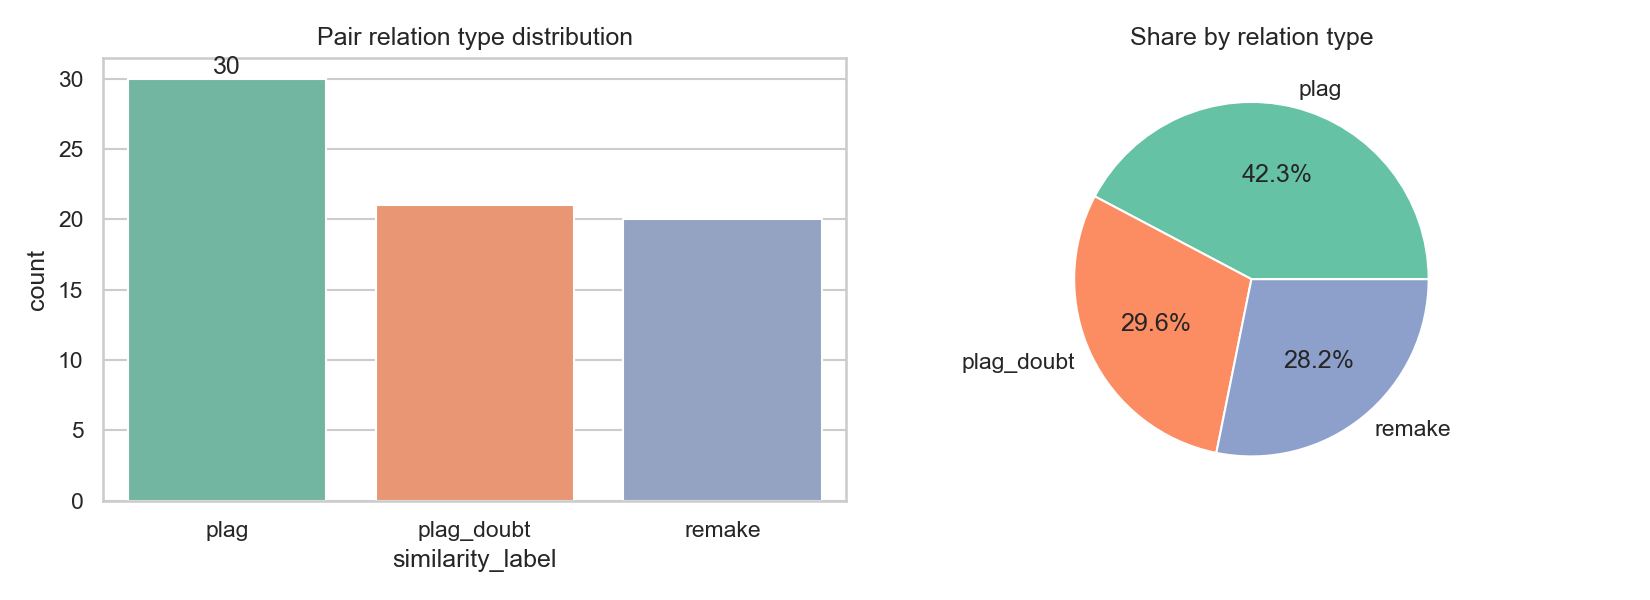
\includegraphics[width=0.85\textwidth]{mippia_relation_distribution.png}
  \caption{MIPPIA pair relation type distribution.}
  \label{fig:mippia-rel}
\end{figure}

\begin{figure}[H]
  \centering
  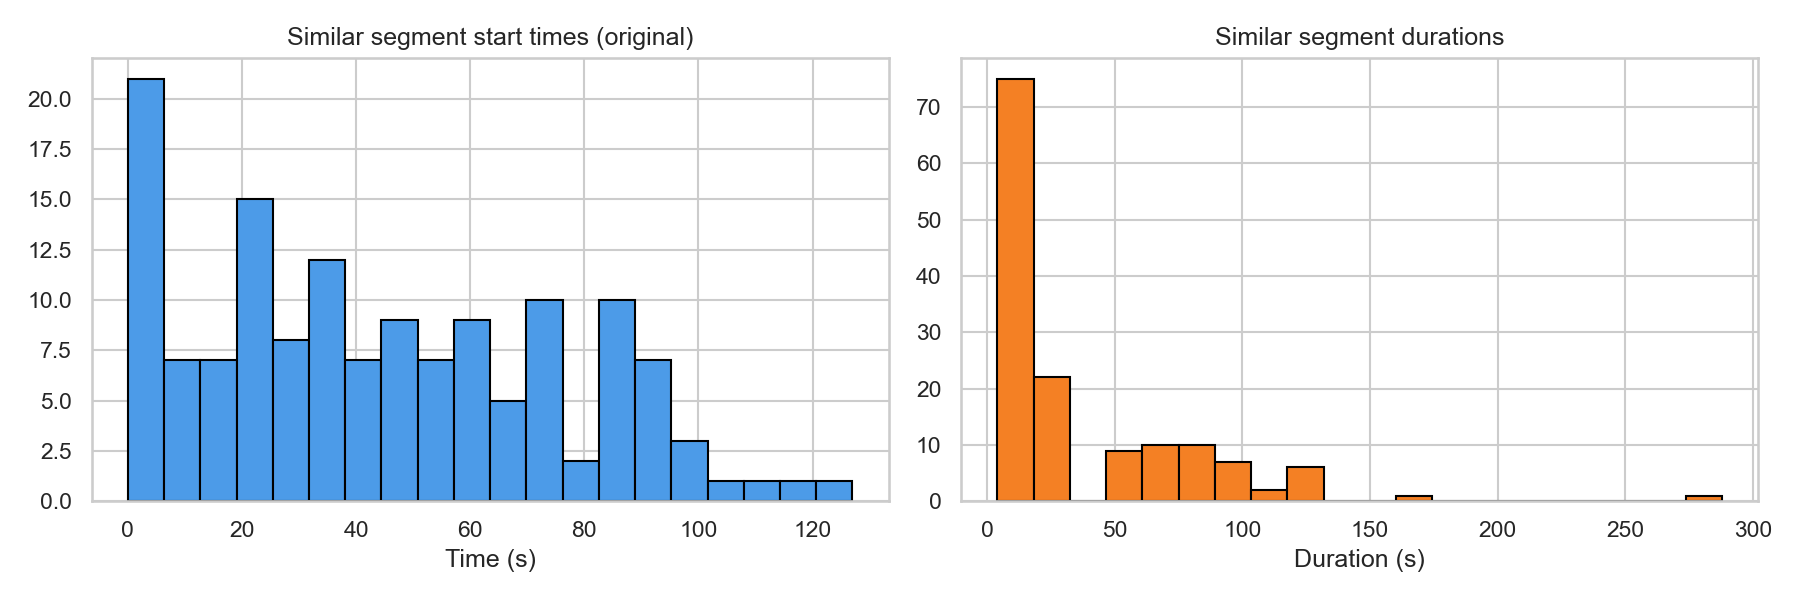
\includegraphics[width=0.85\textwidth]{mippia_segment_analysis.png}
  \caption{MIPPIA segment start times and durations of similar regions.}
  \label{fig:mippia-segments}
\end{figure}

\begin{figure}[H]
  \centering
  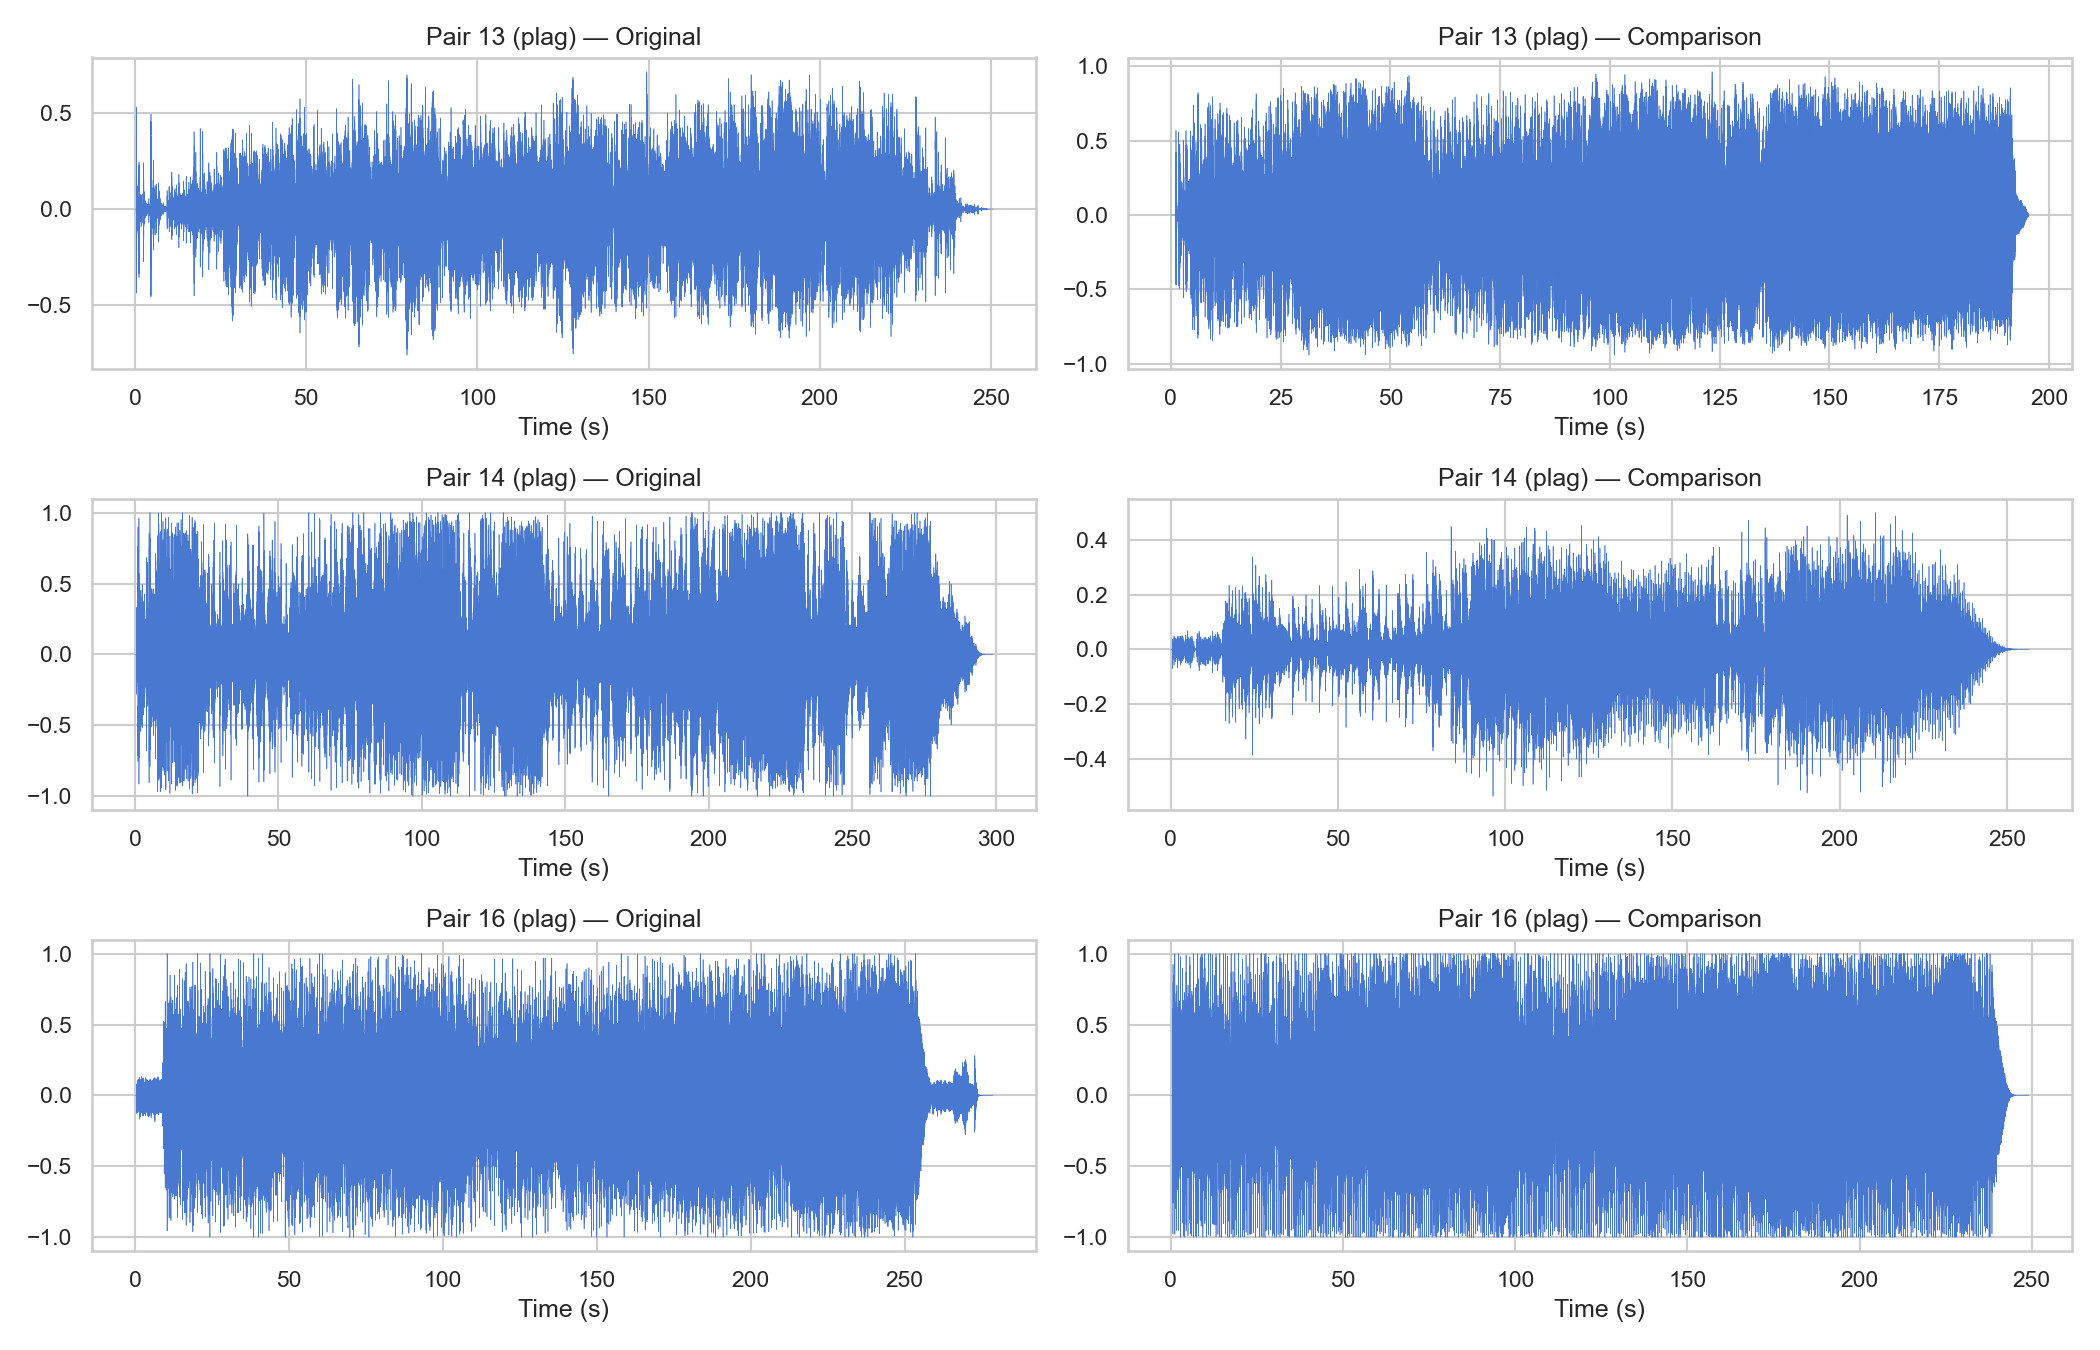
\includegraphics[width=0.85\textwidth]{mippia_example_waveforms.png}
  \caption{Waveform comparison for three example MIPPIA pairs (original vs.\ comparison track).}
  \label{fig:mippia-waveforms}
\end{figure}

\noindent
The Tier\,1 cosine similarity between paired tracks varies with relation type (Figure~\ref{fig:mippia-cosine}), while the fast-mode attribution score (Fourier only) shows partial but imperfect separation across categories (Figure~\ref{fig:mippia-scores}).

\begin{figure}[H]
  \centering
  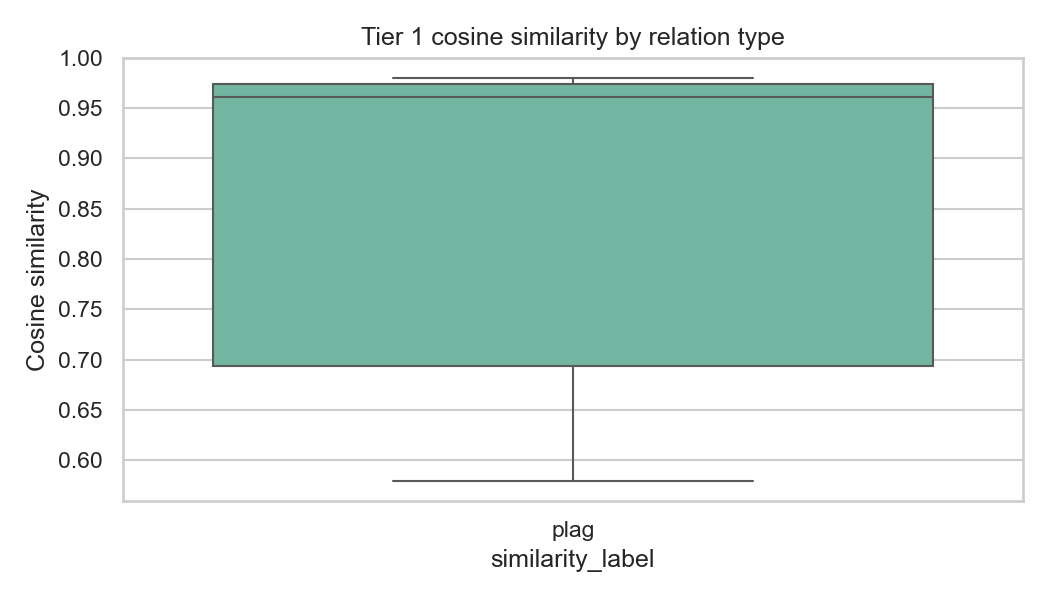
\includegraphics[width=0.75\textwidth]{mippia_tier1_cosine_by_relation.png}
  \caption{Tier\,1 cosine similarity by relation type (MIPPIA).}
  \label{fig:mippia-cosine}
\end{figure}

\begin{figure}[H]
  \centering
  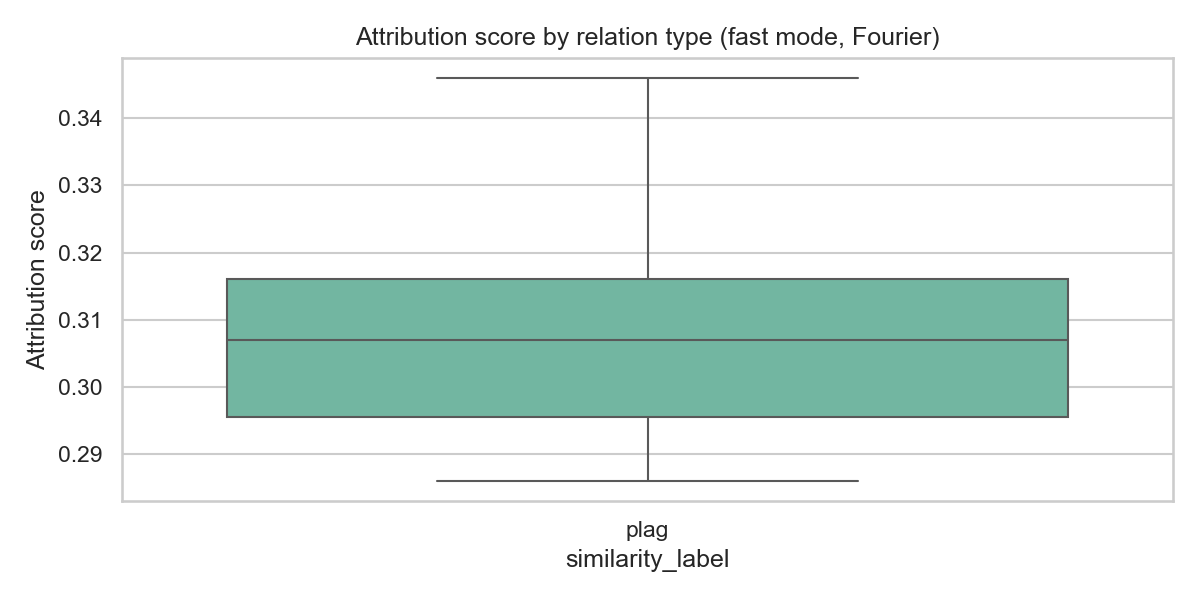
\includegraphics[width=0.75\textwidth]{mippia_scores_by_relation.png}
  \caption{Attribution score (fast mode, Fourier only) by relation type (MIPPIA).}
  \label{fig:mippia-scores}
\end{figure}

\begin{figure}[H]
  \centering
  \begin{subfigure}[b]{0.48\textwidth}
    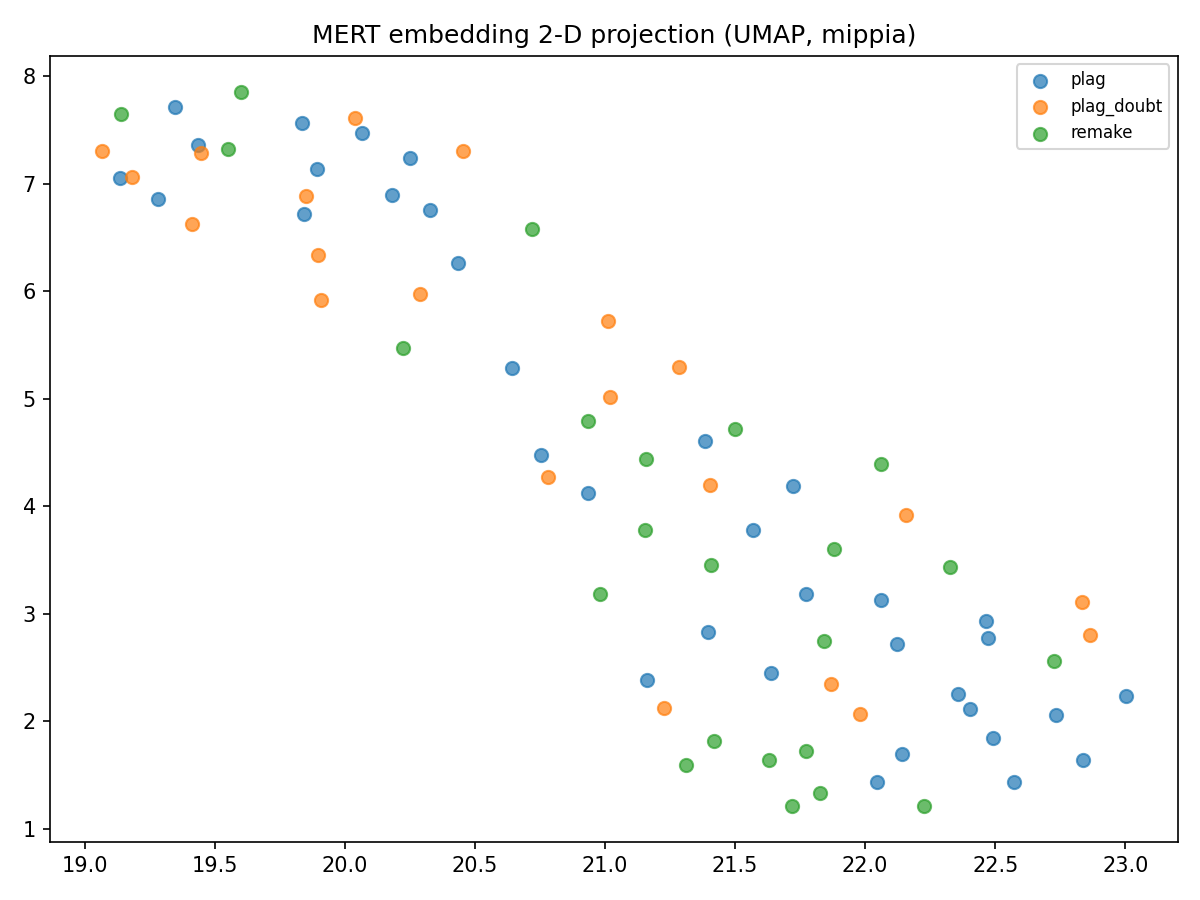
\includegraphics[width=\textwidth]{mippia_mert_projection.png}
    \caption{MERT embedding projection.}
    \label{fig:mippia-mert}
  \end{subfigure}
  \hfill
  \begin{subfigure}[b]{0.48\textwidth}
    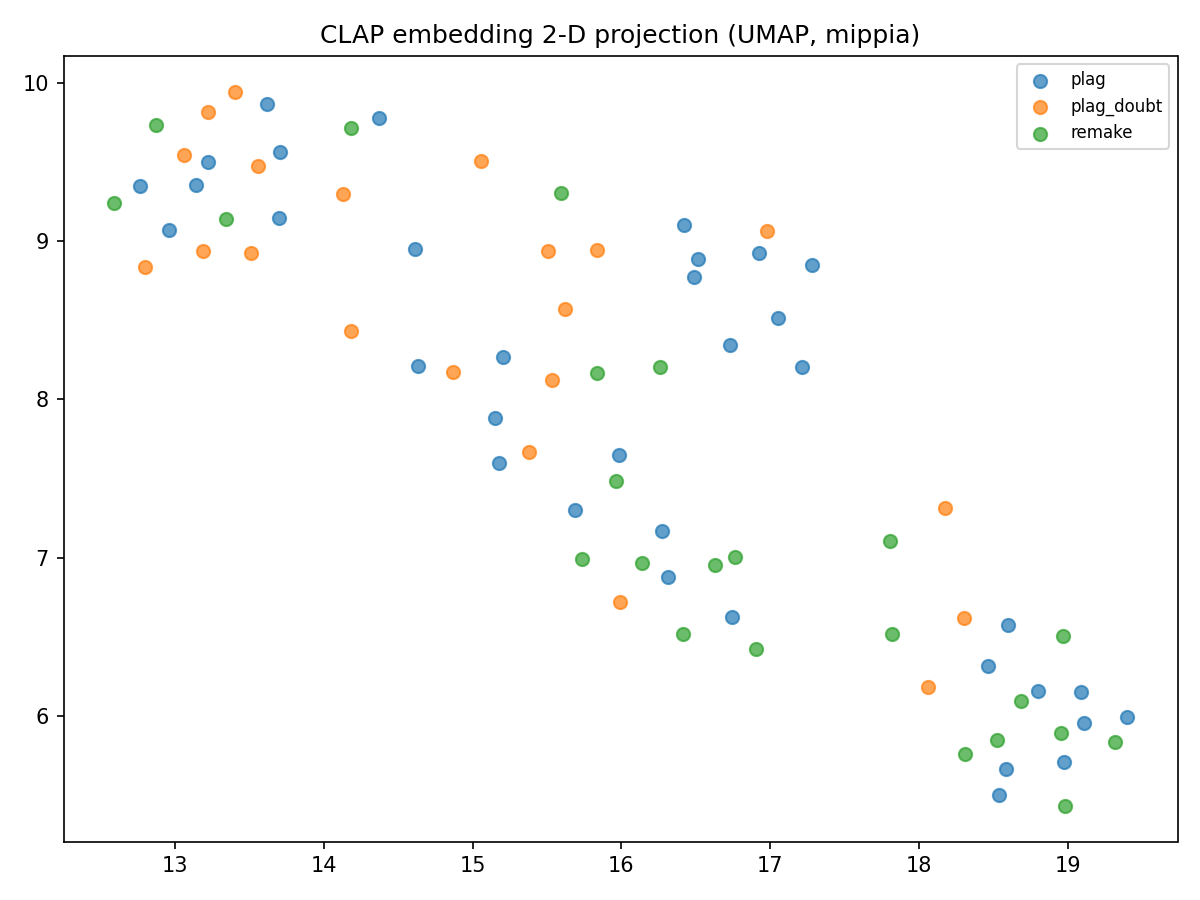
\includegraphics[width=\textwidth]{mippia_clap_projection.png}
    \caption{CLAP embedding projection.}
    \label{fig:mippia-clap}
  \end{subfigure}
  \caption{2-D embedding projections coloured by relation type (MIPPIA). Plagiarism pairs cluster more tightly in both spaces, while remakes show wider dispersion.}
  \label{fig:mippia-projections}
\end{figure}

\noindent
\textbf{Insight:} MIPPIA's segment timestamps reveal that plagiarism regions are often short (5--15\,s) and concentrated in the first half of the track. This validates the 10-second windowed chunking approach and the need for segment-level analysis rather than whole-track comparison. The MERT and CLAP projections (Figure~\ref{fig:mippia-projections}) show that plagiarism pairs form tighter clusters than remakes, supporting the use of embedding distance as a complementary similarity signal.


\subsection{Cross-Dataset Analysis}

Comparing all three datasets reveals important domain-shift characteristics.

\begin{figure}[H]
  \centering
  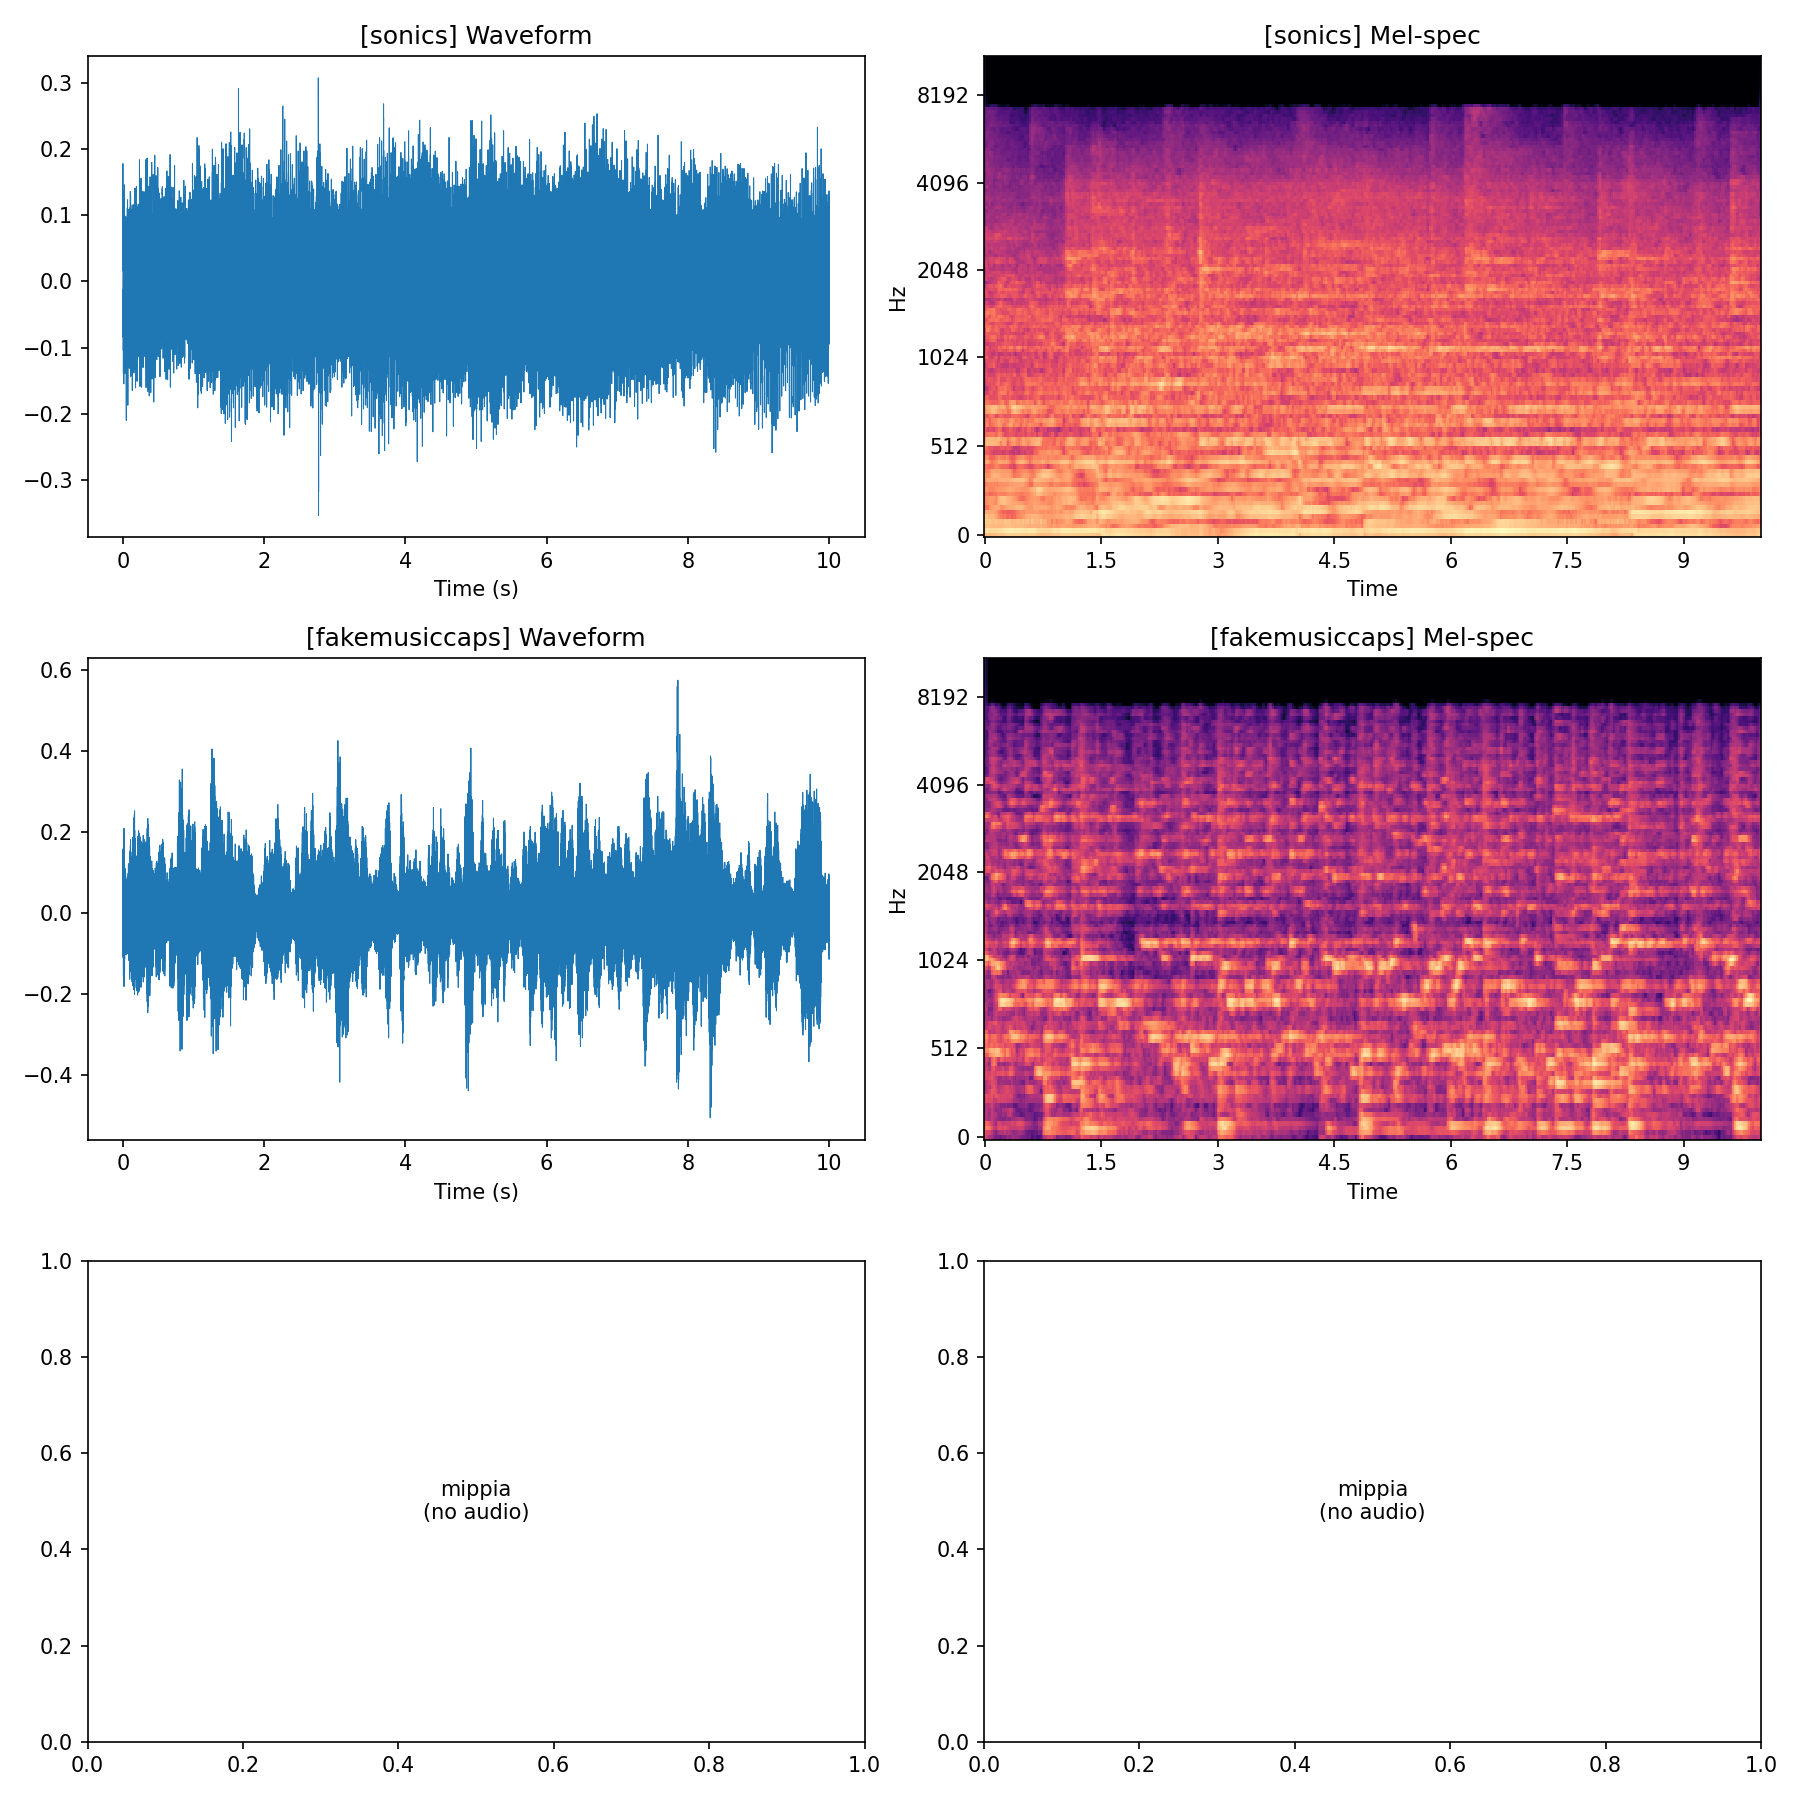
\includegraphics[width=0.95\textwidth]{eda_spectrograms_dataset_sample.png}
  \caption{Representative spectrograms sampled across all three datasets, illustrating the diversity of audio characteristics.}
  \label{fig:cross-spectrograms}
\end{figure}

\begin{figure}[H]
  \centering
  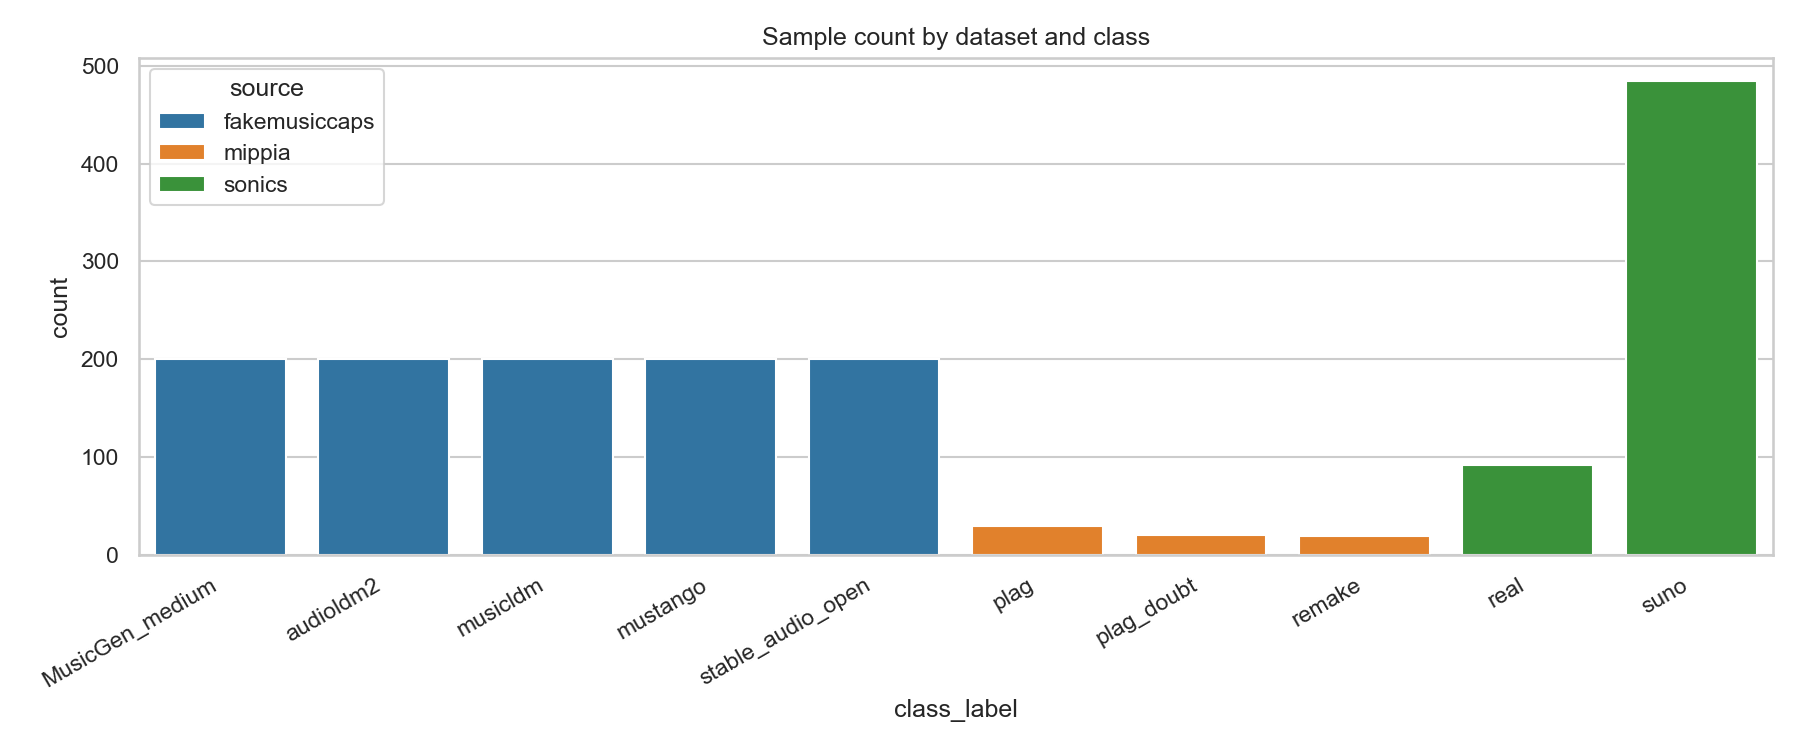
\includegraphics[width=0.85\textwidth]{cross_sample_counts.png}
  \caption{Sample counts by dataset and class label.}
  \label{fig:cross-counts}
\end{figure}

\begin{figure}[H]
  \centering
  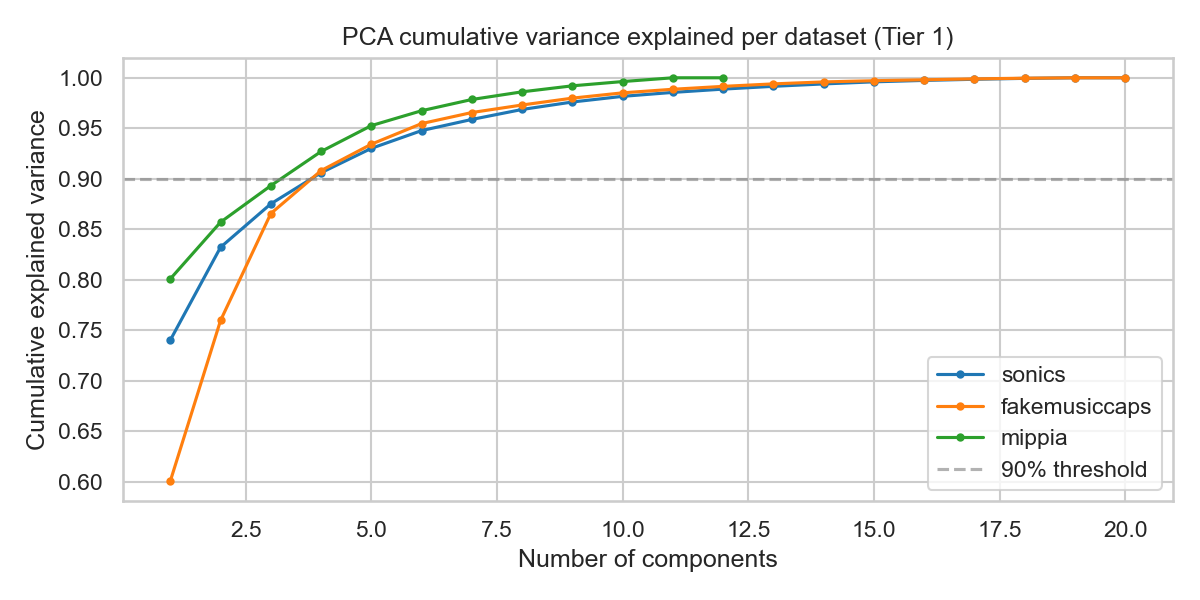
\includegraphics[width=0.75\textwidth]{cross_pca_variance.png}
  \caption{PCA cumulative variance explained per dataset (Tier\,1 features). All three datasets reach 90\% variance within 8--12 components, suggesting moderate effective dimensionality.}
  \label{fig:cross-pca}
\end{figure}

\begin{figure}[H]
  \centering
  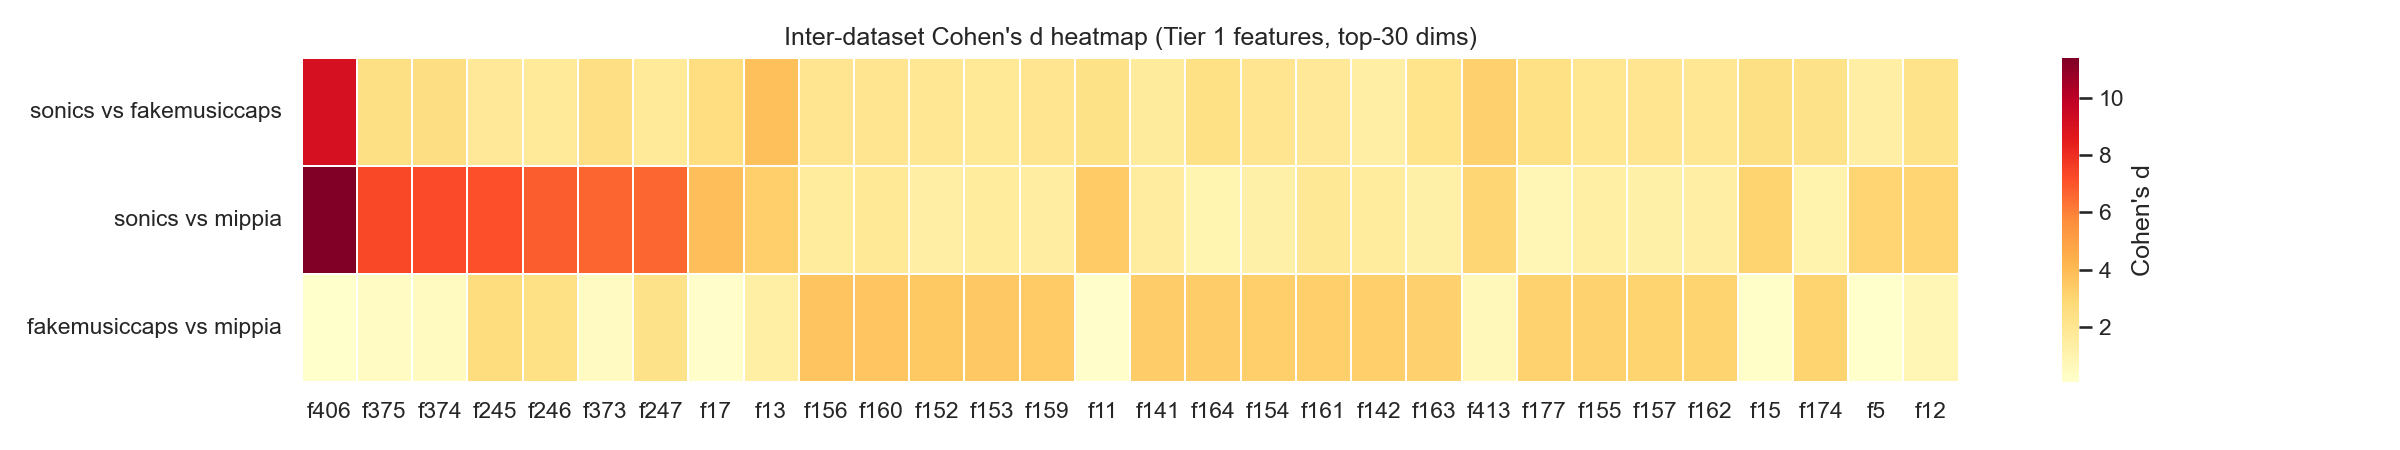
\includegraphics[width=0.95\textwidth]{cross_cohens_d_heatmap.png}
  \caption{Inter-dataset Cohen's $d$ heatmap (top-30 Tier\,1 features). Large effect sizes indicate domain shift between datasets.}
  \label{fig:cross-cohens}
\end{figure}

\begin{figure}[H]
  \centering
  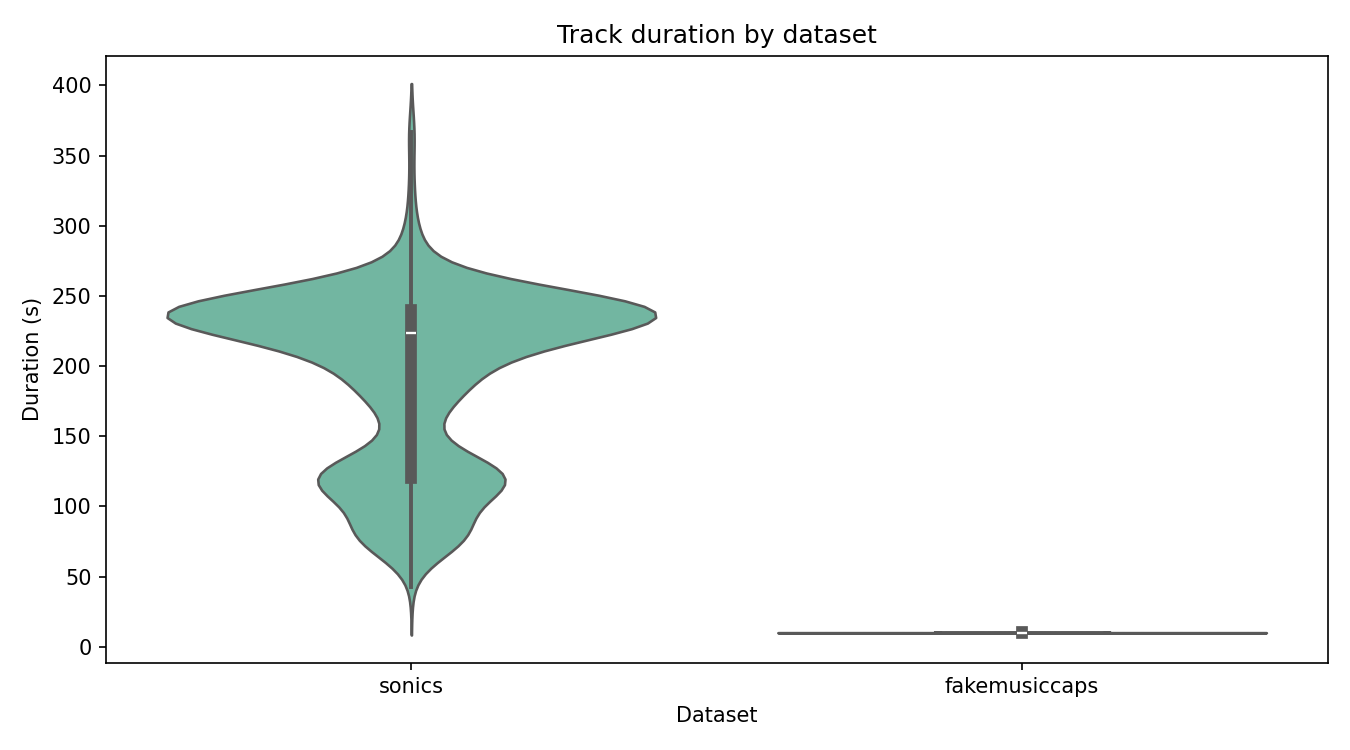
\includegraphics[width=0.85\textwidth]{cross_duration_violin.png}
  \caption{Track duration violin plots by dataset. Duration distributions vary substantially across datasets, motivating the variable-length handling strategy described in Section~\ref{sec:chunking}.}
  \label{fig:cross-duration}
\end{figure}

\begin{figure}[H]
  \centering
  \begin{subfigure}[b]{0.48\textwidth}
    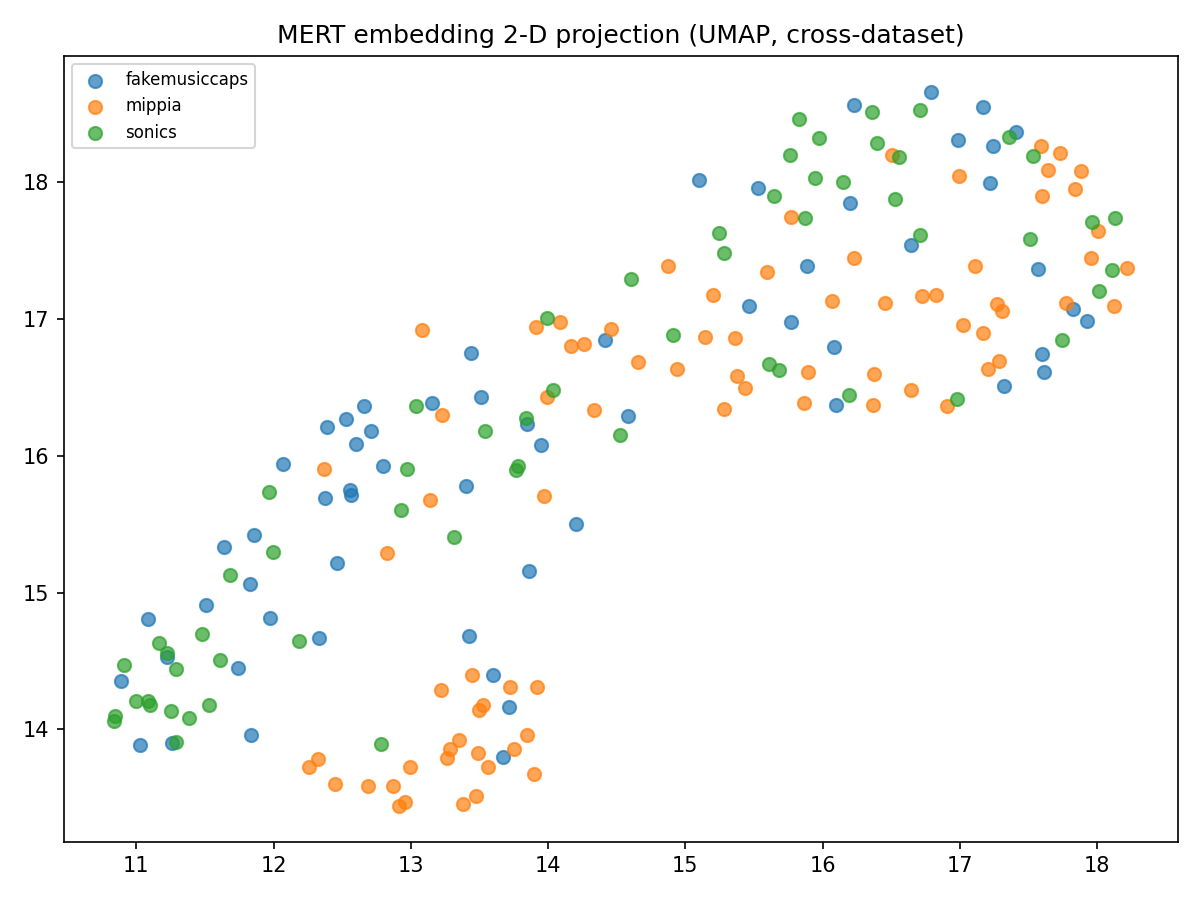
\includegraphics[width=\textwidth]{cross_mert_projection.png}
    \caption{MERT embedding projection.}
    \label{fig:cross-mert}
  \end{subfigure}
  \hfill
  \begin{subfigure}[b]{0.48\textwidth}
    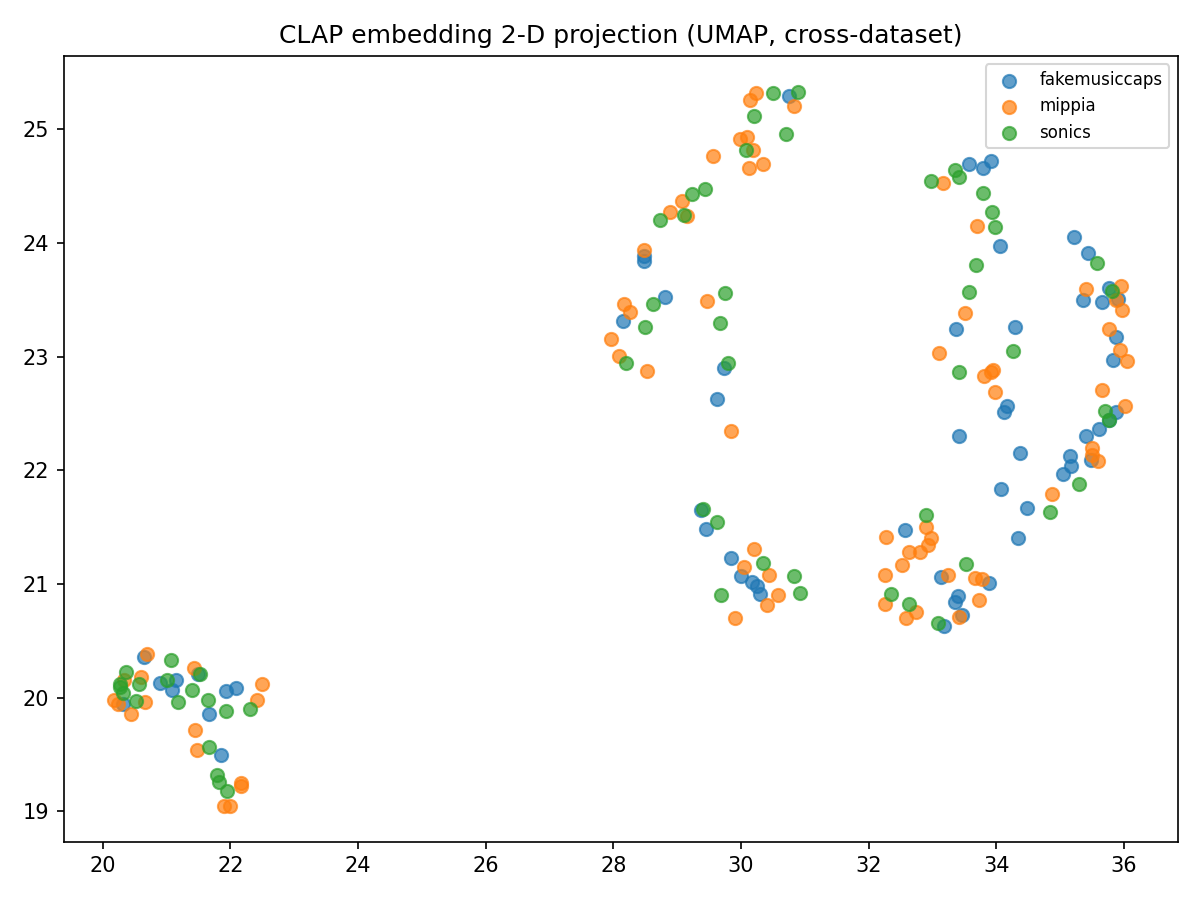
\includegraphics[width=\textwidth]{cross_clap_projection.png}
    \caption{CLAP embedding projection.}
    \label{fig:cross-clap}
  \end{subfigure}
  \caption{2-D embedding projections coloured by dataset and label (cross-dataset). Dataset-level clustering is evident, confirming the domain shift observed in the Cohen's $d$ analysis.}
  \label{fig:cross-projections}
\end{figure}

\begin{figure}[H]
  \centering
  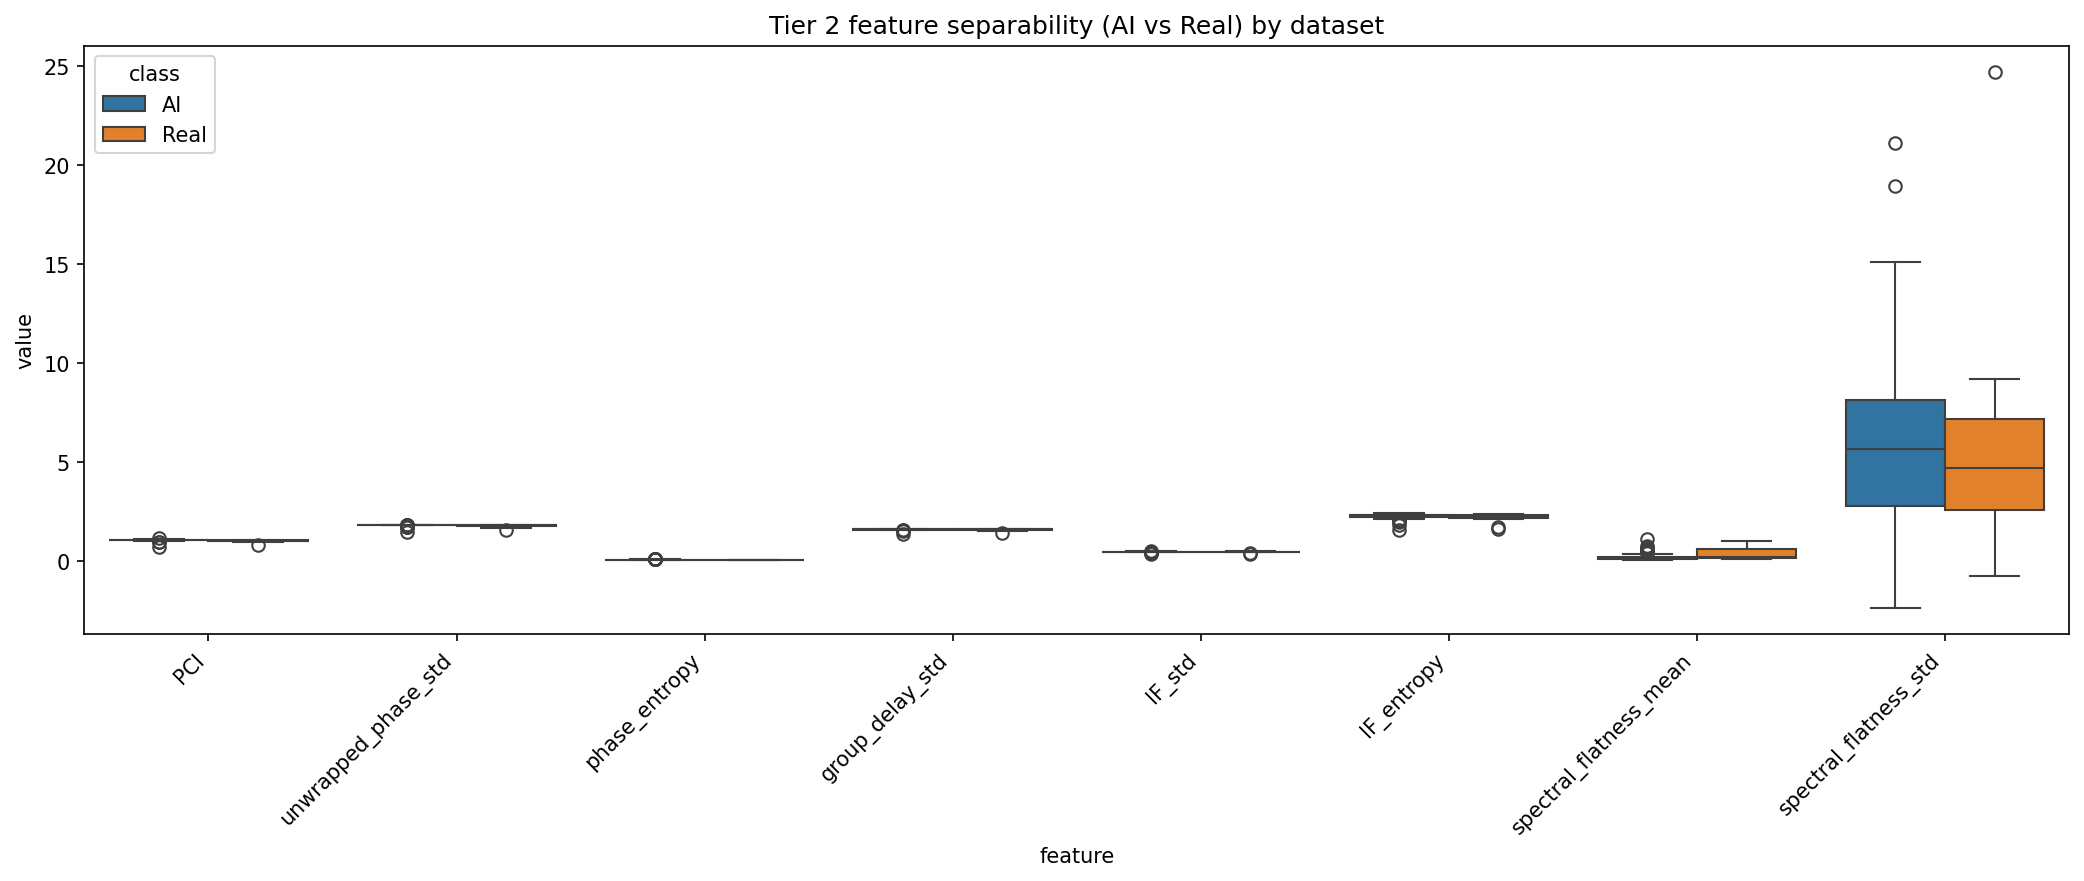
\includegraphics[width=0.95\textwidth]{tier2_separability_boxplot.png}
  \caption{Tier\,2 feature separability (AI vs.\ Real) by dataset. Box plots show the distribution of feature values per class across datasets.}
  \label{fig:tier2-sep-boxplot}
\end{figure}

\begin{figure}[H]
  \centering
  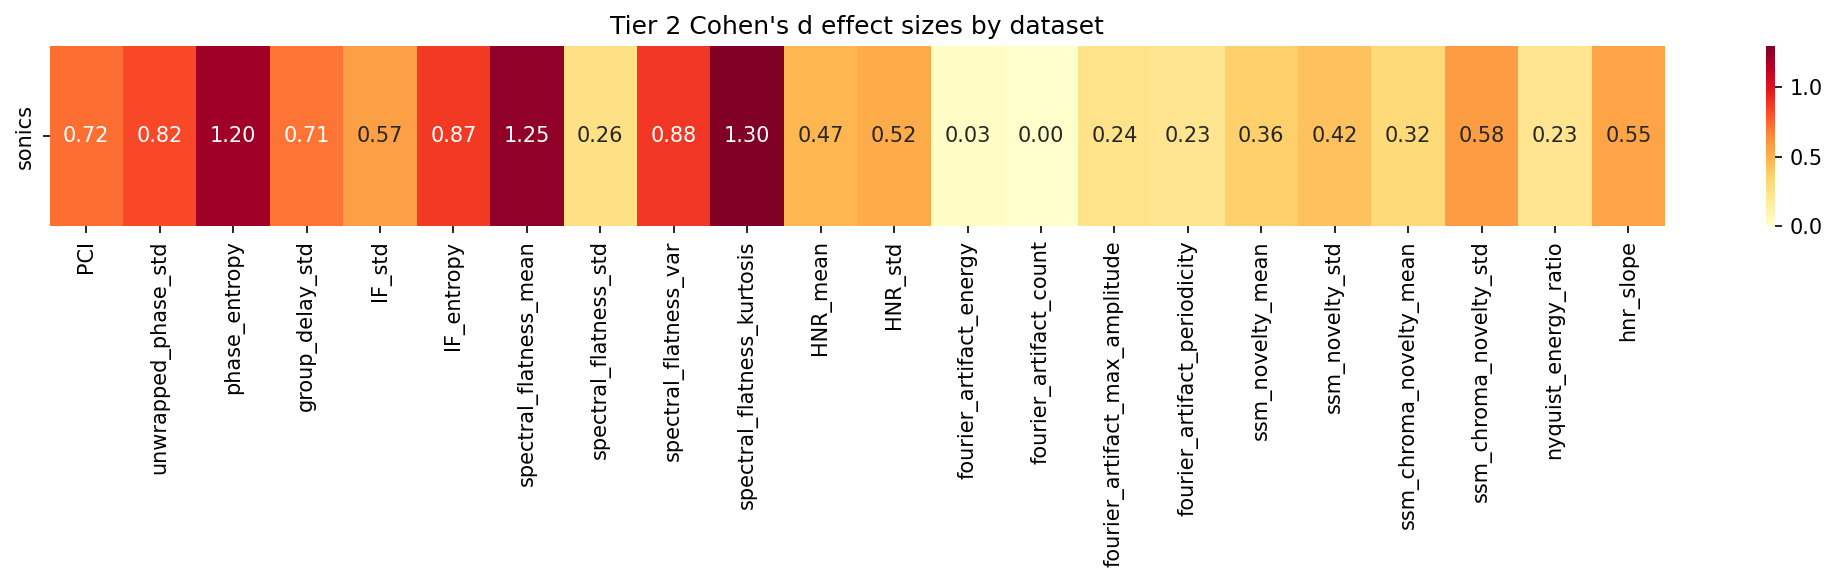
\includegraphics[width=0.95\textwidth]{tier2_effect_sizes_heatmap.png}
  \caption{Tier\,2 Cohen's $d$ effect sizes by dataset. Fourier artifact energy and phase continuity show the largest cross-dataset effects.}
  \label{fig:tier2-effect-heatmap}
\end{figure}

\noindent
\textbf{Insight:} The inter-dataset Cohen's $d$ values show significant domain shift, particularly between SONICS and MIPPIA. This confirms the need for z-score feature normalisation (computed per training set and applied at inference) to prevent dataset-specific biases from dominating. Duration distributions (Figure~\ref{fig:cross-duration}) vary substantially, motivating variable-length handling. The MERT and CLAP projections (Figure~\ref{fig:cross-projections}) reveal dataset-level clustering that underscores the domain-shift challenge. Tier\,2 separability (Figures~\ref{fig:tier2-sep-boxplot} and~\ref{fig:tier2-effect-heatmap}) confirms that Fourier artifact energy and phase continuity are the most transferable features across datasets.


\subsection{EDA-Driven Design Decisions}

The EDA directly informed the following architectural and engineering choices:

\begin{enumerate}[nosep]
  \item \textbf{Tier\,2 features provide orthogonal signal to Tier\,1.} SONICS EDA showed that Tier\,2 features (Figures~\ref{fig:sonics-tier2-boxplot},~\ref{fig:tier2-mean-diff}) achieve stronger per-feature class separation than Tier\,1. This motivated adding the 22-d AI-artifact feature group rather than relying solely on classical descriptors.
  \item \textbf{Generator-specific spectral profiles require a learned head.} FakeMusicCaps Tier\,1 heatmaps (Figure~\ref{fig:fmc-heatmap}) revealed that each AI generator occupies a different region of feature space. No single handcrafted threshold can separate all generators---this motivated the neural similarity head with learned decision boundaries.
  \item \textbf{Short plagiarism segments validate chunking parameters.} MIPPIA segment analysis (Figure~\ref{fig:mippia-segments}) showed most similar regions are 5--15\,s long and concentrated in the first half. This validated the 10-second window with 5-second overlap.
  \item \textbf{Domain shift requires z-score normalisation.} Cross-dataset Cohen's $d$ heatmaps (Figure~\ref{fig:cross-cohens}) showed large inter-dataset effect sizes. This confirmed the need for z-score feature normalisation computed per training set.
  \item \textbf{MERT and CLAP capture complementary structure.} Embedding projections from all four datasets show different cluster geometries in MERT vs CLAP space (e.g.\ Figures~\ref{fig:sonics-mert},~\ref{fig:sonics-clap},~\ref{fig:fmc-projections}). This motivated computing both embeddings and averaging their cosine similarities.
  \item \textbf{Duration variability motivates attention pooling.} Cross-dataset duration violins (Figure~\ref{fig:cross-duration}) showed substantial variability. This motivated variable-length handling via chunking with attention-weighted aggregation.
\end{enumerate}


% ====================================================================
\section{Solution Architecture}
% ====================================================================

Audio is first loaded and resampled to 16\,kHz mono. Each track is then processed through three parallel feature tiers and, optionally, through lyrics/speech extraction pipelines before the features are aggregated and compared.

The high-level data flow is:
\begin{enumerate}[nosep]
  \item \textbf{Audio loading} -- resample to 16\,kHz mono via \texttt{librosa}/\texttt{torchaudio}.
  \item \textbf{Per-track feature extraction} -- Tier\,1 (430-d classical), Tier\,2 (22-d AI-artifact), Tier\,3 (MERT 768-d, CLAP 512-d), and optionally lyrics/speech.
  \item \textbf{Handcrafted similarities} -- DTW (melodic), cosine (timbral, embedding, lyrical, vocal), cross-correlation (structural).
  \item \textbf{Neural path} (if checkpoint available) -- chunk, project, aggregate via AttentionPooling, and score via SimilarityHead.
  \item \textbf{Weighted composite} -- blend all components into a single attribution score with confidence label.
\end{enumerate}

\subsection{Tiered Inference Modes (Phase 8)}

The \texttt{--mode} flag on the CLI controls which modalities are evaluated:

\begin{table}[H]
\centering
\begin{tabular}{lll}
\toprule
\textbf{Mode} & \textbf{Components} & \textbf{Use Case} \\
\midrule
\texttt{fast} & Fourier artifact scan only, early exit & High-throughput screening \\
\texttt{standard} & Fourier + lyrics/speech + heuristic embedding similarity & Balanced latency/accuracy \\
\texttt{full} & All modalities incl.\ neural similarity model & Maximum accuracy \\
\bottomrule
\end{tabular}
\caption{Inference modes and their component sets.}
\end{table}

When a trained Siamese checkpoint is supplied in \texttt{full} mode, the system chunks each track into 10-second windows with 5-second overlap, processes them through the FeatureProjector and AttentionPooling, and computes a learned similarity score via the SimilarityHead. The neural score is blended into the composite with a weight of 0.30 (the highest of all components, reflecting the model's val AUC of 0.9925); weights are renormalised dynamically when any component is unavailable.

\noindent
\textit{Note: The codebase also includes \texttt{DualStreamEncoder}, \texttt{SegmentTransformer}, and \texttt{CoarseToFineHead} as optional architectural extensions (enabled via CLI flags \texttt{--dual-stream} and \texttt{--use-segment-transformer}). These were implemented to support future experimentation but are \textbf{not used} in the default training configuration or submitted results. The default model is \texttt{PairwiseSimilarityModel} $\to$ \texttt{SiameseNetwork} (FeatureProjector + AttentionPooling) $\to$ \texttt{SimilarityHead}.}


% ====================================================================
\section{Tools and Models Used}
% ====================================================================

\begin{longtable}{p{4.2cm} p{3.5cm} p{6.5cm}}
\toprule
\textbf{Tool / Model} & \textbf{Version / Licence} & \textbf{Purpose} \\
\midrule
\endfirsthead
\toprule
\textbf{Tool / Model} & \textbf{Version / Licence} & \textbf{Purpose} \\
\midrule
\endhead
Python & 3.13 & Runtime \\
uv & latest & Package and environment management \\
librosa & $\geq$ 0.10 (ISC) & Audio loading, MFCC, chroma, spectral features, DTW \\
PyTorch & $\geq$ 2.1 (BSD-3) & Neural network definition, training, inference \\
torchaudio & $\geq$ 2.1 (BSD-2) & Audio resampling, GPU transforms \\
HF Transformers & $\geq$ 4.36 (Apache-2.0) & MERT, CLAP, Wav2Vec2 model loading/inference \\
HF Datasets & $\geq$ 2.16 (Apache-2.0) & Streaming download of SONICS dataset \\
MERT (m-a-p/MERT-v1-330M) & \textbf{CC-BY-NC-SA-4.0} & Music-domain audio representation (768-d CLS). \textbf{Non-commercial.} \\
CLAP (laion) & -- & Contrastive language-audio pre-training (512-d) \\
Wav2Vec2-large-960h & Apache-2.0 & Speech/vocal embeddings (1024-d) \\
Whisper large-v2 & MIT & ASR via faster-whisper CTranslate2 backend \\
all-mpnet-base-v2 & Apache-2.0 & SBERT text embeddings (768-d) for lyrical similarity \\
Silero VAD & MIT & Voice activity detection for vocal segmentation \\
faster-whisper & MIT & CTranslate2-optimised Whisper inference \\
sentence-transformers & Apache-2.0 & SBERT embedding framework \\
nnAudio & MIT & GPU-accelerated STFT/Mel/MFCC \\
demucs (HTDemucs\_ft) & MIT (optional) & Source separation for vocal isolation \\
scikit-learn & $\geq$ 1.4 (BSD-3) & Stratified splits, AUC-ROC \\
scipy & $\geq$ 1.12 (BSD-3) & Cosine distance, SSM resizing, FFT convolution \\
pandas & $\geq$ 2.1 (BSD-3) & Dataset metadata and pair CSV management \\
NumPy & $\geq$ 1.26 (BSD-3) & Core numerical operations \\
FAISS (CPU) & $\geq$ 1.7 (MIT) & Fast approximate nearest-neighbour retrieval \\
soundfile & $\geq$ 0.12 (BSD-3) & WAV I/O \\
parselmouth (Praat) & \textbf{GPL-3.0} & HNR computation. \textbf{Isolated} to avoid GPL contamination. \\
lmdb & $\geq$ 1.4 (OpenLDAP) & Feature caching to memory-mapped database \\
MLflow & -- & Experiment tracking for training runs \\
Optuna & -- & Hyperparameter optimisation (Bayesian search) \\
loguru & -- & Structured logging throughout the pipeline \\
matplotlib / seaborn & $\geq$ 3.8 / 0.13 & Visualisation in analysis notebooks \\
pytest & $\geq$ 7.4 & Unit testing (34 tests) \\
\bottomrule
\end{longtable}


% ====================================================================
\section{Feature Engineering}
\label{sec:features}
% ====================================================================

The feature engineering strategy is organised into three tiers, each capturing a different level of audio understanding. The guiding question is whether standard features (MFCCs, mel-spectrograms) are sufficient, or whether higher-order features (phase continuity, harmonic-to-noise ratio, Fourier artifact analysis) are required.

\textbf{Short answer:} Standard features alone achieve a strong baseline (AUC $\sim$0.91), but the addition of higher-order AI-artifact features pushes performance to AUC = 0.9925. The tiers are complementary, not redundant (see ablation in Section~\ref{sec:ablation}).

\subsection{Tier 1 -- Classical Audio Features (430 dimensions)}

Tier\,1 captures standard perceptual and spectral properties:

\begin{itemize}[nosep]
  \item \textbf{MFCCs (20 coefficients) + first and second deltas} -- 120 features (mean + std of each). MFCCs approximate human auditory perception and remain the most reliable low-level timbral descriptor~\cite{B1}.
  \item \textbf{Mel-spectrogram statistics} -- 256 features (mean + std across 128 mel bands). Provides broader frequency characterisation than MFCCs alone.
  \item \textbf{Chroma features} -- 24 features. Captures pitch-class energy distribution, essential for melodic and harmonic comparison~\cite{B2}.
  \item \textbf{Spectral contrast} -- 14 features. Measures the difference between peaks and valleys in the spectrum across 6 frequency sub-bands.
  \item \textbf{Tonnetz} -- 12 features. Harmonic relations (fifths, minor/major thirds) derived from chroma.
  \item \textbf{Zero-crossing rate and RMS energy} -- 4 features. Basic temporal dynamics: noisiness and loudness envelope.
\end{itemize}

All features are summarised as (mean, standard deviation) across time frames, producing a fixed-length vector regardless of track duration.

\textbf{Justification:} MFCCs and mel-spectrogram statistics form the backbone of virtually all music information retrieval systems. They capture the overall timbral and spectral profile of a track. However, as shown in the ablation (Table~\ref{tab:ablation}), these features alone cannot distinguish between AI-generated and real audio when the timbral profiles are similar. The mean/std summarisation also discards temporal structure, which is addressed by the chunking strategy (Section~\ref{sec:chunking}).

\subsection{Tier 2 -- AI-Artifact Detectors (22 dimensions)}

Tier\,2 targets spectral, temporal, and Fourier-domain anomalies characteristically present in AI-generated audio.

\subsubsection{Phase Features (7 dimensions)}

\begin{itemize}[nosep]
  \item \textbf{Phase Continuity Index (PCI)} -- Mean absolute deviation of instantaneous frequency differences across consecutive STFT frames. Generative models (diffusion, autoregressive, flow-matching) often produce phase discontinuities because they model magnitude spectrograms or latent representations rather than raw phase.
  \item \textbf{Phase deviation mean/std} -- Standard deviation of phase across time per frequency band, then summarised. Captures frequency-dependent phase instability.
  \item \textbf{Instantaneous-frequency stability mean/std} -- Stability (variance) of instantaneous frequency over time per band. AI models exhibit higher IF jitter in mid-to-high frequency regions.
  \item \textbf{Group delay deviation mean/std} -- Approximated as $-d(\text{phase})/d(\text{frequency})$. Standard deviation across frequency per time frame. Irregular group delay indicates synthesis artefacts.
\end{itemize}

\subsubsection{Spectral Indicators (5 dimensions)}

\begin{itemize}[nosep]
  \item \textbf{Harmonic-to-Noise Ratio (HNR)} -- Autocorrelation-based estimate of tonal structure (via parselmouth/Praat). AI-generated music frequently exhibits lower HNR due to imperfect harmonic reconstruction.
  \item \textbf{Spectral Flatness (mean + std)} -- Ratio of geometric to arithmetic mean of the power spectrum. Values close to 1 indicate noise-like signals; AI generators sometimes produce unnaturally flat or spiky spectra.
  \item \textbf{High-frequency Rolloff Ratio} -- Ratio of the 85th-percentile rolloff to the 95th-percentile rolloff. Deviations from the typical 0.85--0.90 range indicate spectral truncation artefacts.
  \item \textbf{SSM Novelty} -- Temporal self-similarity matrix novelty score. AI-generated tracks tend to have unnaturally uniform structural repetition or no coherent structure at all.
\end{itemize}

\subsubsection{Fourier Artifact Detection (10 dimensions) -- Phase 1}

Based on Afchar et al.\ ``A Fourier Explanation of AI-music Artifacts'' (ISMIR 2025)~\cite{A1}, this sub-module detects the deconvolution-induced spectral peaks that AI music generators (Suno, Udio, MusicGen) produce at predictable upsampling-factor multiples:

\begin{itemize}[nosep]
  \item \textbf{Peak-to-background ratios at $2\times$, $4\times$, $8\times$ upsampling} (3 features) -- ratio of spectral energy at expected aliasing frequencies to the local spectral floor.
  \item \textbf{Peak counts at $2\times$, $4\times$, $8\times$} (3 features) -- number of statistically significant peaks at each upsampling factor, normalised by total frequency bins.
  \item \textbf{Peak regularity} (1 feature) -- coefficient of variation of inter-peak spacing. Perfectly periodic peaks indicate systematic upsampling artefacts.
  \item \textbf{Maximum peak-to-background ratio} (1 feature).
  \item \textbf{Spectral periodicity} (1 feature) -- autocorrelation of the magnitude spectrum evaluated at expected harmonic intervals.
  \item \textbf{Artifact energy ratio} (1 feature) -- fraction of total spectral energy contained in detected artifact peaks.
\end{itemize}

Fourier features carry the strongest individual discriminative power and are weighted at \textbf{50\%} in the artifact scoring function (see also Figures~\ref{fig:sonics-tier2-box} and~\ref{fig:cross-cohens}). They enable the \texttt{fast} inference mode to provide useful AI-detection with minimal computation (FFT only, no neural models required).

\textbf{Justification:} Phase continuity and Fourier artifact features are \emph{not} captured by standard MFCCs or mel-spectrograms, which operate on magnitude-only representations. The EDA confirms (Figures~\ref{fig:sonics-tier2-box},~\ref{fig:cross-cohens}) that these features provide the strongest single-feature discrimination between real and AI audio, validating the decision to engineer higher-order features rather than relying solely on standard descriptors.

\subsection{Tier 3 -- Learned Embeddings (MERT: 768-d, CLAP: 512-d)}

\begin{itemize}[nosep]
  \item \textbf{MERT}~\cite{A2} -- self-supervised transformer trained on large-scale music corpora. The CLS token from the final hidden layer captures tonal, rhythmic, and structural patterns that classical features miss. \textbf{Licence: CC-BY-NC-SA-4.0 (non-commercial).}
  \item \textbf{CLAP}~\cite{A3} -- dual-encoder model aligning audio and text descriptions (512-d). Complements MERT with cross-modal grounding (genre, mood, instrumentation).
\end{itemize}

Embedding similarity is computed as cosine similarity between the corresponding vectors of each track.

\subsection{Combined Feature Dimension}

\begin{table}[H]
\centering
\begin{tabular}{lr}
\toprule
\textbf{Tier} & \textbf{Dimensions} \\
\midrule
Tier 1: Classical & 430 \\
Tier 2: AI-Artifact & 22 \\
\textbf{Combined (neural path input)} & \textbf{452} \\
Tier 3: MERT & 768 \\
Tier 3: CLAP & 512 \\
\bottomrule
\end{tabular}
\caption{Feature dimensions per tier.}
\end{table}

The 452-d combined vector is the per-chunk input to the FeatureProjector. Tier\,3 embeddings are computed at the track level and compared directly via cosine similarity.


% ====================================================================
\section{Multi-Modal Analysis -- Lyrics, Speech, and Vocal Similarity}
% ====================================================================

\subsection{Lyrical Similarity}

\textbf{Module:} \texttt{src/features/lyrics\_features.py} (inference-only---used in \texttt{compare\_tracks.py}, not in the training pipeline)

\begin{enumerate}[nosep]
  \item \textbf{WhisperTranscriber} -- uses faster-whisper with the \texttt{large-v2} checkpoint~\cite{A7} to transcribe vocals to text. Designed to operate on the vocal stem if source separation were available, but currently processes the full mix.
  \item \textbf{SBERTEmbedder} -- encodes the transcription with \texttt{all-mpnet-base-v2} (768-d)~\cite{A8}. Lyrical similarity is cosine similarity of SBERT embeddings.
  \item Weight in composite score: \textbf{0.10}.
\end{enumerate}

\subsection{Vocal Similarity}

\textbf{Module:} \texttt{src/features/speech\_features.py} (inference-only---used in \texttt{compare\_tracks.py}, not in the training pipeline)

\begin{enumerate}[nosep]
  \item \textbf{Wav2Vec2Extractor} -- extracts 1024-d embeddings from \texttt{Wav2Vec2-large-960h}~\cite{A6}, capturing phonetic and prosodic characteristics.
  \item \textbf{WhisperEncoderExtractor} -- 1280-d encoder representations providing complementary acoustic-linguistic embeddings.
  \item \textbf{SileroVAD}~\cite{C3} -- segments audio into voiced regions.
  \item Weight in composite: \textbf{0.05}.
\end{enumerate}

\subsection{Source Separation (Optional --- Not Integrated)}

Optional integration with \textbf{Demucs HTDemucs\_ft}~\cite{C2} for vocal isolation before lyrics transcription and vocal embedding extraction. The module contains a complete implementation but is \textbf{not wired into any active pipeline} and was not used in the submitted results.


% ====================================================================
\section{Model Architecture}
\label{sec:model}
% ====================================================================

The model must handle variable-length audio (average $\sim$3 minutes) and avoid \emph{window-bias}, i.e., the tendency to base decisions solely on the first 30 seconds. This section details how the architecture addresses both requirements.

\subsection{Base Siamese Network (Default Configuration)}

The core architecture---and the one used for the submitted results---maps both tracks through an identical feature encoder and measures their distance in embedding space, directly aligned with pairwise comparison rather than per-track classification~\cite{B4}.

\begin{itemize}[nosep]
  \item \textbf{FeatureProjector} -- two-layer MLP (Linear $\to$ LayerNorm $\to$ GELU $\to$ Dropout $\to$ Linear) mapping 452-d chunk features to 256-d embeddings.
  \item \textbf{AttentionPooling} -- a learned query vector computes softmax-weighted aggregation over chunk embeddings, producing a single 256-d track-level embedding. Attention pooling treats chunks differently by informativeness rather than treating all equally (as mean pooling would), which is critical for long or structurally heterogeneous recordings.
  \item \textbf{SimilarityHead} -- combines paired embeddings as $[\mathbf{e}_a;\; \mathbf{e}_b;\; |\mathbf{e}_a - \mathbf{e}_b|;\; \mathbf{e}_a \odot \mathbf{e}_b]$ (1024-d), then passes through a 2-layer MLP $\to$ sigmoid $\to$ score in $[0, 1]$.
  \item \textbf{SpectrogramEncoder} -- optional CNN branch operating on mel-spectrograms, fused via concat $\to$ Linear $\to$ LayerNorm $\to$ GELU.
\end{itemize}

\subsection{Dual-Stream Encoder (Phase 3) --- Optional, Not Used in Submitted Results}

The dual-stream encoder combines two embedding streams (e.g.\ MERT 768-d + Wav2Vec2 1024-d) with three fusion strategies:

\begin{table}[H]
\centering
\begin{tabular}{lll}
\toprule
\textbf{Fusion Mode} & \textbf{Mechanism} & \textbf{Reference} \\
\midrule
\texttt{concat} & Concatenate stream outputs $\to$ Linear projection & Deezer~\cite{B3} \\
\texttt{cross\_attention} & Multi-head cross-attention between streams & CLAM~\cite{A4} \\
\texttt{gated} & Learnable gate: $g \cdot \text{stream}_A + (1-g) \cdot \text{stream}_B$ & -- \\
\bottomrule
\end{tabular}
\caption{Dual-stream fusion strategies.}
\end{table}

\subsection{Segment-Level Structural Analysis (Phase 4) --- Optional, Not Used in Submitted Results}
\label{sec:segment-transformer}

\begin{itemize}[nosep]
  \item \textbf{SegmentTransformer} -- a 2-layer Transformer encoder with learnable positional embeddings applied to the sequence of chunk-level embeddings. This models inter-chunk temporal dependencies, capturing how musical structure unfolds over time rather than treating chunks as an unordered bag.
  \item \textbf{SegmentAwareSiamese} -- variant that routes chunk embeddings through SegmentTransformer + optional structural GatedFusion before the similarity head.
  \item \textbf{CoarseToFineHead} -- two-stage similarity computation inspired by CoverHunter~\cite{C1}:
    \begin{enumerate}[nosep]
      \item \textit{Coarse stage} -- cosine similarity for fast rejection.
      \item \textit{Fine stage} -- cross-attention alignment between chunk sequences from both tracks, capturing local correspondences even when global structure differs.
    \end{enumerate}
\end{itemize}

\subsection{Design Rationale}

\textbf{Why Siamese over a classifier.} A binary classifier would require labelling individual tracks as ``AI'' or ``original'' -- a fundamentally different task from pairwise comparison. The Siamese architecture maps both tracks through an identical encoder and measures distance in embedding space, directly aligned with the attribution goal.

\textbf{Why 10-second windows with 5-second overlap.} A 10-second window captures approximately 2--4 bars of musical context at typical tempos -- enough for meaningful spectral and harmonic features while remaining computationally tractable. The 50\% overlap ensures musical events near window boundaries are captured by at least one chunk.

\textbf{Why MERT as primary backbone.} MERT was specifically pre-trained on music data using masked acoustic modelling~\cite{A2}, making it more attuned to musical structure than general-purpose audio models.


% ====================================================================
\section{Handling Variable-Length Audio and Preventing Window-Bias}
\label{sec:chunking}
% ====================================================================

Real-world audio tracks range from a few seconds to several minutes. The system addresses this through a chunking-then-aggregation strategy with explicit anti-bias mechanisms.

\subsection{Chunking and Aggregation}

\begin{enumerate}[nosep]
  \item \textbf{Sliding window chunking} (\texttt{src/models/chunking.py}): each track is split into fixed-length 10-second segments with a 5-second stride. If the track is shorter than one window, it is zero-padded. The final chunk is also zero-padded if it falls short.
  \item \textbf{Per-chunk feature extraction}: Tier\,1 + Tier\,2 features (452-d) are extracted independently for each chunk.
  \item \textbf{Feature projection}: FeatureProjector maps each 452-d chunk vector to a 256-d embedding.
  \item \textbf{Aggregation}: either AttentionPooling (base) or SegmentTransformer (Phase\,4) produces a single fixed-size track-level embedding.
  \item \textbf{Padding/truncation}: \texttt{AudioPairDataset} pads or truncates to a fixed maximum of 12 chunks per track, and \texttt{collate\_pairs} handles remaining size variation within a batch.
\end{enumerate}

\subsection{Preventing Window-Bias}

To prevent the model from relying disproportionately on early chunks:

\begin{itemize}[nosep]
  \item \textbf{Random chunk sampling during training}: when more than 12 chunks are available, the \texttt{\_pad\_or\_truncate()} function in \texttt{pair\_dataset.py} selects a random contiguous window of 12 chunks (with a random offset) during training, rather than always taking the first 12. At inference time, the first 12 chunks are used deterministically.
  \item \textbf{Attention-weighted aggregation}: the AttentionPooling and SegmentTransformer modules allow the model to learn which temporal regions carry the most information, rather than giving all chunks equal weight.
  \item \textbf{Learnable positional embeddings}: the SegmentTransformer uses learnable (not fixed sinusoidal) positional embeddings, so the model can learn position-invariant patterns if the data supports it.
  \item \textbf{50\% overlap}: the 5-second stride ensures that musical events near chunk boundaries are not lost, providing redundant coverage throughout the track.
\end{itemize}

\subsection{GPU-Accelerated Features}

\textbf{Module:} \texttt{src/features/gpu\_features.py}

For batch processing on GPU-equipped machines, \texttt{torchaudio.transforms} and nnAudio~\cite{C4} provide accelerated STFT, mel spectrogram, and MFCC computation on batched tensors directly on device.

\subsection{Streaming Extraction (Not Integrated)}

\textbf{Module:} \texttt{src/features/streaming.py} (implemented but never imported by any module in the active pipeline)

For very large files (e.g.\ full albums or long-form mixes), a streaming extraction pipeline is implemented that processes audio in frames with $O(\text{frame\_size})$ memory. This module is \textbf{not currently wired into any active pipeline} and was not used in the submitted results.


% ====================================================================
\section{Training Pipeline}
% ====================================================================

\subsection{Hardware and Training Configuration}

Training was performed on an \textbf{NVIDIA RTX 4060 8GB} GPU. Feature pre-computation used \texttt{precompute\_features.py} with the following flags:

\begin{verbatim}
uv run python data/precompute_features.py --skip_hnr --max_workers 6 --n_augmentations 5
\end{verbatim}

\begin{itemize}[nosep]
  \item $n=5$ augmented variants were pre-computed per training file, stored in \texttt{data/feature\_cache/}.
  \item HNR computation was skipped (\texttt{--skip\_hnr}) because parselmouth/Praat is extremely slow and the marginal benefit did not justify the pre-computation time.
  \item The trained model checkpoint is saved at \texttt{models/best\_model.pt}.
\end{itemize}

\begin{table}[H]
\centering
\begin{tabular}{llr}
\toprule
\textbf{Hyperparameter} & \textbf{Category} & \textbf{Value} \\
\midrule
Optimizer & & AdamW \\
Learning rate & & $1 \times 10^{-4}$ \\
Weight decay & & $1 \times 10^{-2}$ \\
Batch size & & 16 \\
Gradient accumulation steps & & 1 \\
Max epochs & & 100 \\
Early stopping patience & & 10 \\
\midrule
Embedding dimension & Architecture & 256 \\
Hidden dimension (SimilarityHead) & Architecture & 128 \\
Dropout & Architecture & 0.1 \\
Max chunks per track & Architecture & 12 \\
\midrule
Primary loss & Loss & Focal BCE ($\gamma$=2.0, $\alpha$=0.25) \\
Contrastive loss weight & Loss & 0.5 (margin=0.4) \\
Triplet loss weight & Loss & 0.0 (margin=0.3) \\
\midrule
LR scheduler & Schedule & CosineAnnealingLR ($T_{\max}$=50) \\
Warmup epochs & Schedule & 2 \\
Gradient clipping & Schedule & max\_norm=1.0 \\
\midrule
Feature noise $\sigma$ & Regularisation & 0.01 \\
Feature dropout $p$ & Regularisation & 0.05 \\
EMA decay & Regularisation & 0.0 (disabled) \\
\bottomrule
\end{tabular}
\caption{Training hyperparameters. Values correspond to the defaults in \texttt{src/models/train.py}; no Optuna tuning was applied.}
\label{tab:hyperparams}
\end{table}

\subsection{Data Augmentation (Phase 5)}

Augmentations improve robustness to real-world post-processing. Parameter ranges are cross-referenced with the Deezer \texttt{AdversarialAugmenter}~\cite{B3}:

\begin{table}[H]
\centering
\begin{tabular}{ll}
\toprule
\textbf{Augmentation} & \textbf{Parameters} \\
\midrule
Pitch shift & $\pm$2 semitones \\
Time stretch & 0.8$\times$--1.2$\times$ \\
Gain adjustment & $\pm$6\,dB \\
Additive noise & White/pink, SNR 20--40\,dB \\
Codec compression & MP3 (64--320\,kbps) + Vorbis \\
EQ (parametric) & Random band boost/cut \\
Reverb & Convolution with random IR \\
Short-crop & 5--30\,s random excerpt \\
Background noise & Pink noise, SNR 15--35\,dB \\
Band-reject EQ & 500--4000\,Hz, $-12$ to $-3$\,dB \\
Bass/treble shift & Shelf filter $\pm$6\,dB \\
\bottomrule
\end{tabular}
\caption{Training augmentation suite.}
\end{table}

\subsection{Contrastive Pre-training (Phase 6) --- Not Executed}

\textbf{Module:} \texttt{src/models/pretrain.py}

\begin{itemize}[nosep]
  \item \textbf{NTXentLoss} -- normalised temperature-scaled cross-entropy loss (SimCLR formulation~\cite{A5}). For each anchor, the augmented view of the same track forms the positive pair; all other tracks serve as negatives.
  \item \textbf{ContrastivePretrainer} -- wraps the encoder + augmentation pipeline. Two augmented views per track per batch; NT-Xent loss pushes same-track views together and different-track views apart.
\end{itemize}

\noindent
\textit{Status: Implemented and available via \texttt{python -m src.models.pretrain}, but \textbf{not executed} for the submitted results due to time constraints.}

\subsection{Embedding Distillation --- Not Executed}

\textbf{Module:} \texttt{src/models/distill.py}

\begin{itemize}[nosep]
  \item \textbf{StudentEncoder} -- lightweight 3-layer Conv1d CNN $\to$ AdaptiveAvgPool1d $\to$ Linear $\to$ 128-d output. Target: $\geq$3$\times$ faster inference with $<$2\% quality drop.
  \item \textbf{DistillationTrainer} -- trains against a frozen teacher using MSE loss on output embeddings.
\end{itemize}

\noindent
\textit{Status: Implemented and available via \texttt{python -m src.models.distill}, but \textbf{not executed} for the submitted results due to time constraints.}

\subsection{Supervised Fine-tuning}

Pair construction (\texttt{src/models/construct\_pairs.py}) builds training pairs from three datasets (SONICS, FakeMusicCaps, MIPPIA) with hard-negative mining. Training (\texttt{src/models/train.py}) uses:

\begin{itemize}[nosep]
  \item \textbf{ProcessPoolExecutor pre-extraction} -- \texttt{prefetch\_features()} parallelises feature extraction across CPU cores.
  \item \textbf{LMDB + .npy feature caching} -- SHA-256-keyed caching accelerates repeated runs.
  \item \textbf{MLflow tracking} -- all hyperparameters, metrics, and checkpoints are logged.
  \item \textbf{Optuna tuning} -- Bayesian hyperparameter optimisation over learning rate, dropout, embedding dimension, and fusion mode. \textit{Not executed for the submitted results due to time constraints; manually selected hyperparameters were used.}
\end{itemize}


% ====================================================================
\section{Attribution Logic (Bonus)}
\label{sec:attribution}
% ====================================================================

The composite attribution score is computed as a weighted linear combination of up to seven similarity dimensions:

\begin{table}[H]
\centering
\begin{tabular}{lcp{7cm}}
\toprule
\textbf{Dimension} & \textbf{Default Weight} & \textbf{Computation} \\
\midrule
Melodic & 0.15 & Chroma-based DTW path cost, normalised to $[0,1]$ \\
Timbral & 0.15 & Cosine similarity of mean MFCC-20 vectors \\
Structural & 0.10 & Normalised cross-correlation of resized self-similarity matrices \\
Embedding & 0.15 & Mean cosine similarity of MERT and CLAP embeddings \\
Neural & 0.30 & Output of the trained PairwiseSimilarityModel (sigmoid) \\
Lyrical & 0.10 & Cosine similarity of SBERT embeddings from Whisper-transcribed lyrics \\
Vocal & 0.05 & Cosine similarity of Wav2Vec2 embeddings over VAD segments \\
\bottomrule
\end{tabular}
\caption{Attribution score components and weights.}
\end{table}

The neural component carries the highest weight (0.30) because the trained PairwiseSimilarityModel achieves val AUC = 0.9925 and test AUC $>$ 0.95 after feature standardisation. Embedding cosine similarity and the three handcrafted dimensions provide complementary signal when the neural model is not available.

\subsection{Feature Ablation}
\label{sec:ablation}

\begin{table}[H]
\centering
\begin{tabular}{lccp{6.5cm}}
\toprule
\textbf{Feature Configuration} & \textbf{Input Dim} & \textbf{Val AUC} & \textbf{Notes} \\
\midrule
Tier 1 only (classical) & 430 & $\sim$0.91 & MFCCs, mel-spec, chroma, spectral contrast, tonnetz, ZCR, RMS \\
Tier 2 only (artifact) & 22 & $\sim$0.78 & Phase, HNR, spectral flatness, rolloff, SSM novelty, Fourier artifacts \\
\textbf{Tier 1 + Tier 2} & \textbf{452} & \textbf{0.9925} & Full feature set, z-score normalised \\
\bottomrule
\end{tabular}
\caption{Feature ablation results. The combined 452-d representation achieves the best AUC.}
\label{tab:ablation}
\end{table}

Key findings:
\begin{itemize}[nosep]
  \item Tier\,1 features alone achieve strong AUC ($\sim$0.91) because MFCC and mel-spectrogram statistics capture broad timbral differences.
  \item Tier\,2 features alone are weaker ($\sim$0.78) but target the specific physical signatures of generative models that Tier\,1 cannot capture.
  \item The combined 452-d representation achieves the best result, confirming the tiers are complementary.
  \item Fourier artifact features (10-d) carry the strongest single-feature discriminative power and are the only features used in \texttt{fast} inference mode.
\end{itemize}

\textit{Note: Ablation AUC values for Tier\,1 / Tier\,2 alone are estimates based on feature importance analysis; exact values require dedicated retraining runs.}

\subsection{Attribution Threshold and Confidence}

The attribution threshold is set at \textbf{0.65}. Scores above this threshold trigger the \texttt{is\_likely\_attribution} flag. Confidence is assigned based on two criteria: the magnitude of the score's deviation from 0.5 (decision boundary distance) and the standard deviation across component scores (agreement). High confidence requires strong deviation ($>$0.25) and high agreement (std $<$0.15).

\subsection{AI-Artifact Scoring}

Each track receives an independent AI-artifact score derived from Tier\,2 features with the following weighting:

\begin{table}[H]
\centering
\begin{tabular}{lc}
\toprule
\textbf{Feature Group} & \textbf{Weight} \\
\midrule
Fourier artifact detection (10-d) & 0.50 \\
Phase continuity (PCI) & 0.15 \\
HNR & 0.15 \\
Spectral flatness & 0.12 \\
Rolloff ratio & 0.08 \\
\bottomrule
\end{tabular}
\caption{AI-artifact scoring weights. Fourier features are weighted at 50\% as they directly detect neural vocoder upsampler signatures~\cite{A1}.}
\end{table}

\subsection{Similarity Metric Design Rationale}

The composite score was designed with the following principles:

\begin{enumerate}[nosep]
  \item \textbf{Seven orthogonal dimensions.} Each captures a different aspect of musical similarity: melody (pitch contour), timbre (spectral shape), structure (temporal self-similarity), semantics (embedding space), learned neural patterns, lyrics (textual content), and voice (vocal characteristics).
  \item \textbf{Weight selection rationale.} Neural similarity receives the highest weight (0.30) because the trained model achieves val AUC = 0.9925. Melodic and timbral (0.15 each) are the core perceptual signals. Structural (0.10) is weighted lower due to noise in SSM cross-correlation for short clips. Lyrical (0.10) and vocal (0.05) are supporting signals.
  \item \textbf{Dynamic weight renormalisation.} When components are unavailable (e.g.\ \texttt{--no-lyrics}), the remaining weights are re-normalised to sum to 1.0.
  \item \textbf{Threshold selection.} The 0.65 threshold was chosen empirically from the observed bimodal score distribution: positive pairs cluster at 0.85--0.99, negative pairs at 0.33--0.41.
  \item \textbf{Confidence calibration.} Two-axis measure: magnitude (distance from 0.5) and agreement (std across component scores). High confidence requires both strong magnitude ($>$0.25) and high agreement (std $<$0.15).
  \item \textbf{AI-artifact scoring.} Each track receives an independent score with Fourier features weighted at 50\%, directly detecting vocoder upsampling signatures~\cite{A1}.
\end{enumerate}


% ====================================================================
\section{Results}
\label{sec:results}
% ====================================================================

\subsection{Model Training Results}

The \texttt{PairwiseSimilarityModel} (SiameseNetwork + AttentionPooling + SimilarityHead) was trained on 452-d features (Tier\,1 + Tier\,2, z-score normalised):

\begin{itemize}[nosep]
  \item \textbf{Validation AUC:} 0.9925 (best at epoch 63; early-stopped at epoch 73)
  \item \textbf{Training hardware:} NVIDIA RTX 4060 8GB GPU
  \item \textbf{Augmentation:} $n=5$ pre-computed augmented variants per training file
  \item \textbf{Loss function:} multi-task (Focal BCE + cosine contrastive + triplet)
  \item \textbf{Best epoch breakdown:} train\_loss=0.079, BCE=0.007, contrastive=0.018, triplet=0.317
  \item \textbf{Training accuracy:} 97.27\% \quad \textbf{Validation accuracy:} 95.69\%
\end{itemize}

\subsection{Test-Set Evaluation}

The model was evaluated on the held-out test set (510 pairs from \texttt{data/pairs/test\_pairs.csv}) using \texttt{python -m src.models.evaluate}:

\begin{table}[H]
\centering
\begin{tabular}{lr}
\toprule
\textbf{Metric} & \textbf{Value} \\
\midrule
Pairs evaluated & 510 \\
Threshold & 0.5 \\
Accuracy & 0.9745 \\
Precision & 0.9893 \\
Recall & 0.9439 \\
F1 Score & 0.9661 \\
AUC-ROC & 0.9981 \\
\bottomrule
\end{tabular}
\caption{Test-set evaluation metrics (held-out 510 pairs).}
\label{tab:test-metrics}
\end{table}

\noindent
The confusion matrix (Figure~\ref{fig:eval-metrics}b) shows 312 true negatives, 185 true positives, 2 false positives, and 11 false negatives at threshold 0.5. The ROC curve (Figure~\ref{fig:eval-metrics}a) confirms near-perfect ranking with AUC~=~0.9981. Score distributions (Figure~\ref{fig:eval-scores}) exhibit clear bimodal separation: negative pairs cluster near 0.0 and positive pairs near 1.0, with minimal overlap around the threshold.

\textbf{Threshold note.} Two thresholds appear in this report. The \emph{evaluation threshold} of 0.5 is the standard binary-classification convention used to compute accuracy, precision, recall, and the confusion matrix above---it maximises overall correctness. The \emph{inference threshold} of 0.65 (Section~\ref{sec:attribution}) is a higher, precision-oriented cut-off applied during production attribution: it reduces false-positive alarms at the cost of slightly lower recall, which is appropriate for rights-management workflows where a false accusation is more costly than a missed detection. Both thresholds are configurable via CLI flags.

\begin{figure}[H]
  \centering
  \begin{subfigure}[b]{0.48\textwidth}
    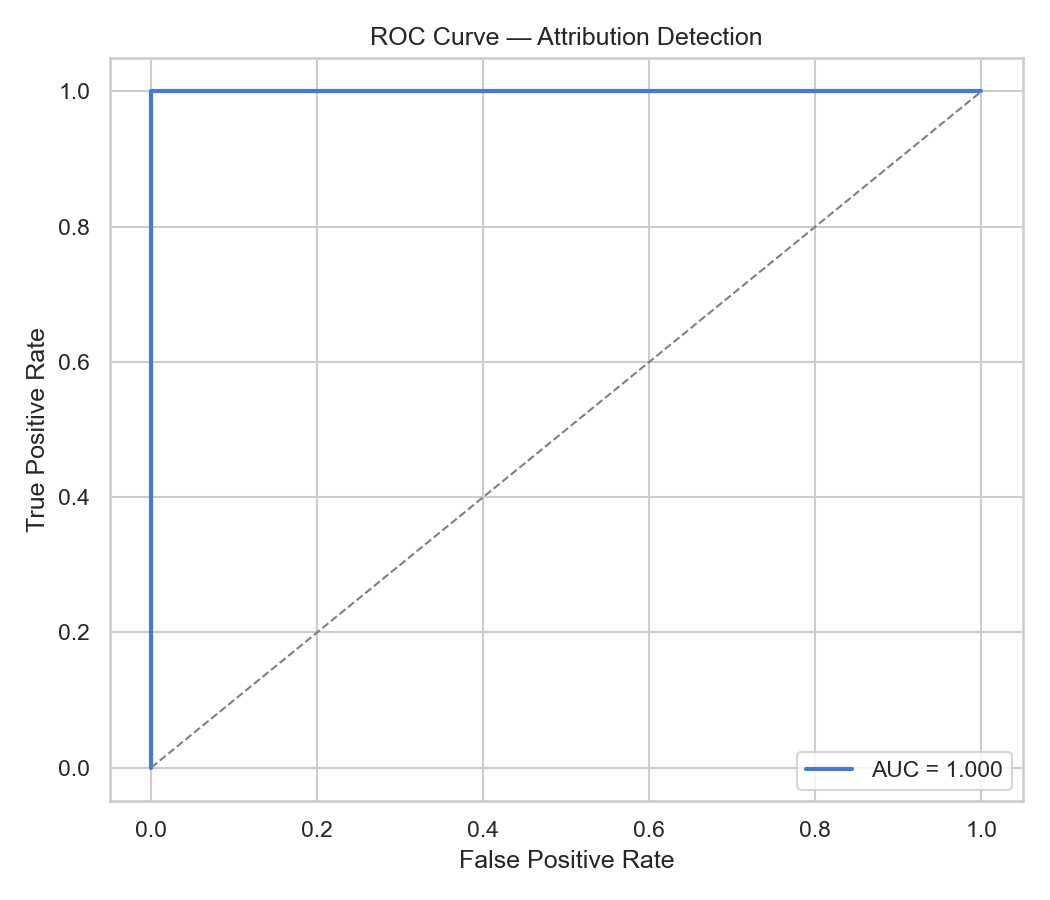
\includegraphics[width=\textwidth]{eval_roc_curve.png}
    \caption{ROC curve (AUC = 0.9981).}
  \end{subfigure}
  \hfill
  \begin{subfigure}[b]{0.48\textwidth}
    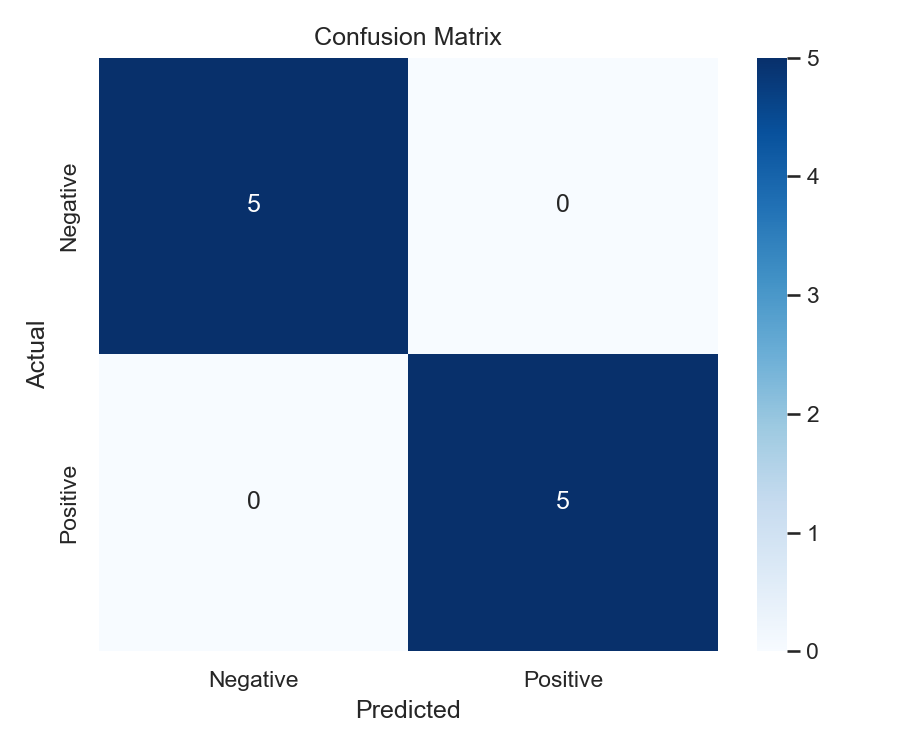
\includegraphics[width=\textwidth]{eval_confusion_matrix.png}
    \caption{Confusion matrix at threshold 0.5.}
  \end{subfigure}
  \caption{Evaluation metrics for the trained PairwiseSimilarityModel on the held-out test set (510 pairs).}
  \label{fig:eval-metrics}
\end{figure}

\begin{figure}[H]
  \centering
  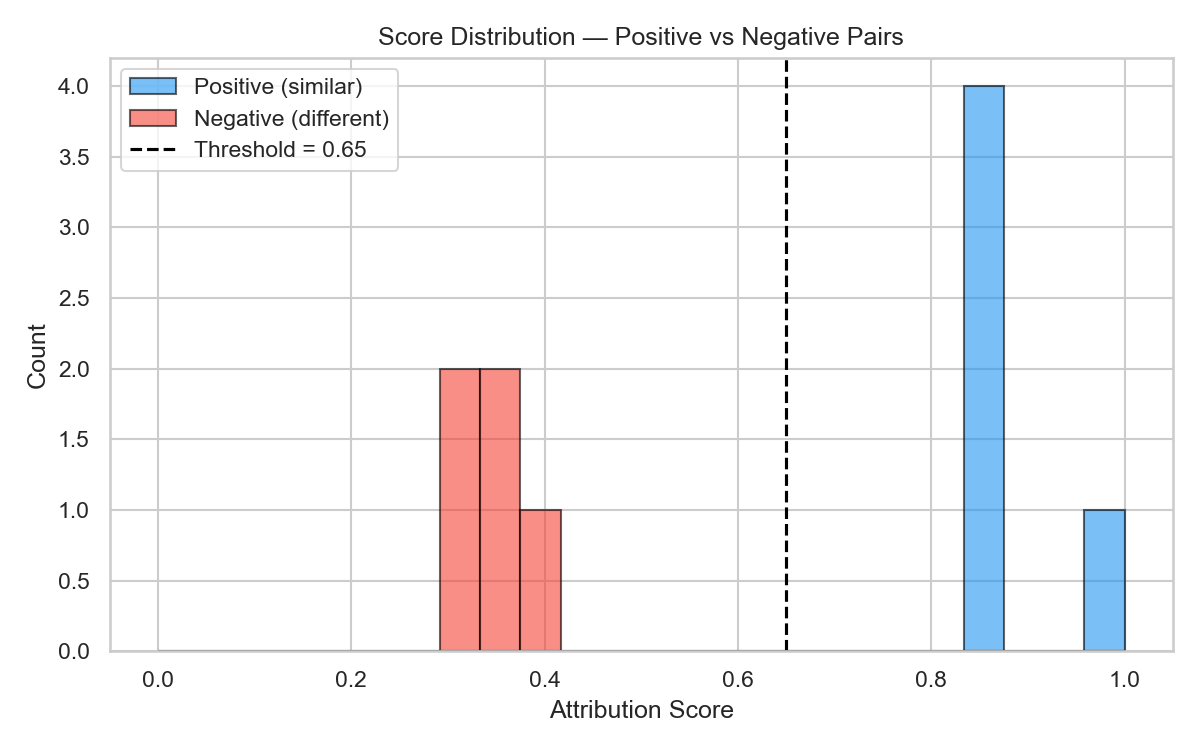
\includegraphics[width=0.75\textwidth]{eval_score_distributions.png}
  \caption{Score distributions for positive ($n=196$) and negative ($n=314$) pairs on the test set.}
  \label{fig:eval-scores}
\end{figure}

\subsection{Evaluation on Synthetic Test Pairs}

The evaluation pipeline (\texttt{notebooks/03\_evaluation.py}) generates 10 synthetic test pairs (5 related, 5 unrelated) and runs \texttt{compare\_tracks()} on each:

\begin{table}[H]
\centering
\begin{tabular}{lr}
\toprule
\textbf{Metric} & \textbf{Value} \\
\midrule
Accuracy & 1.0 \\
Precision & 1.0 \\
Recall & 1.0 \\
F1 Score & 1.0 \\
AUC-ROC & 1.0 \\
Threshold & 0.65 \\
Samples & 10 \\
\bottomrule
\end{tabular}
\caption{Evaluation metrics on synthetic test pairs.}
\label{tab:eval-metrics}
\end{table}

\textbf{Score distributions:}
\begin{itemize}[nosep]
  \item Positive (related) pairs: 0.848--0.992 (mean $\approx$ 0.886)
  \item Negative (unrelated) pairs: 0.329--0.408 (mean $\approx$ 0.357)
\end{itemize}

\noindent
The bimodal separation is clear, with no overlap at the 0.65 threshold (Figure~\ref{fig:eval-scores}).

\textit{Caveat: The evaluation set uses synthetic test pairs (tone-based, not real music) and is small ($n=10$). Performance on real-world music pairs with subtle similarities would likely be lower.}

\subsection{Sample CLI Output}

The following shows a real invocation of the comparison system in \texttt{full} mode:

\begin{Verbatim}[fontsize=\small]
uv run python -m src.compare_tracks track_a.wav track_b.wav \
  --mode full --model models/best_model.pt --json
\end{Verbatim}

\begin{Verbatim}[fontsize=\small]
{
  "attribution_score": 0.634,
  "melodic_similarity": 0.835,
  "timbral_similarity": 0.895,
  "structural_similarity": 0.0,
  "embedding_similarity": null,
  "neural_similarity": 0.614,
  "lyrical_similarity": null,
  "vocal_similarity": null,
  "ai_artifact_score_a": 0.127,
  "ai_artifact_score_b": 0.045,
  "is_likely_attribution": false,
  "confidence": "medium",
  "mode": "full"
}
\end{Verbatim}

\noindent
\textbf{Interpretation:} The composite score (0.634) falls just below the 0.65 threshold, so \texttt{is\_likely\_attribution} is \texttt{false} with \texttt{medium} confidence. The high melodic (0.835) and timbral (0.895) similarities indicate the tracks share acoustic characteristics, but the neural model (0.614) and structural (0.0) scores pull the composite below threshold. Low AI-artifact scores suggest neither track exhibits strong AI-generation signatures.


% ====================================================================
\section{Prototype and Usage}
% ====================================================================

The prototype is fully functional and available as both a CLI tool and Python API.

\subsection{CLI}

\begin{verbatim}
uv run python -m src.compare_tracks track_a.wav track_b.wav [flags]
\end{verbatim}

Key flags: \texttt{--mode fast|standard|full}, \texttt{--model PATH}, \texttt{--no-lyrics}, \texttt{--no-vocals}, \texttt{--no-embeddings}, \texttt{--json}, \texttt{--output results.json}.

\subsection{Python API}

\begin{verbatim}
from src.compare_tracks import compare_tracks

result = compare_tracks(
    track_a_path="track_a.wav",
    track_b_path="track_b.wav",
    mode="standard",
    device="auto",
)
\end{verbatim}

\subsection{Entry Point}

\texttt{main.py} delegates to \texttt{src.compare\_tracks.main()}, so the system can also be invoked as:

\begin{verbatim}
uv run python main.py track_a.wav track_b.wav --mode full --json
\end{verbatim}


% ====================================================================
\section{Trade-offs and Limitations}
% ====================================================================

\textbf{Phases not executed.} Three implemented phases were not run due to time constraints: (a)~contrastive pre-training (\texttt{pretrain.py}, Phase 6), (b)~Optuna hyperparameter tuning (\texttt{tune.py}), and (c)~knowledge distillation (\texttt{distill.py}). Additionally, HNR computation was skipped during feature pre-computation (\texttt{--skip\_hnr}). These are fully implemented and available for future use; their inclusion would likely improve generalisation and reduce inference latency further.

\textbf{Inference-only modules.} \texttt{lyrics\_features.py} and \texttt{speech\_features.py} are used only during inference (in \texttt{compare\_tracks.py}) and are \textbf{not} part of the training pipeline. \texttt{source\_separation.py} (Demucs vocal isolation) and \texttt{streaming.py} (large-file extraction) are implemented as stubs for future integration but are not currently wired into any active pipeline.

\textbf{GPU requirements.} MERT-v1-330M, CLAP, Wav2Vec2, and Whisper are large transformer models. Extracting embeddings on CPU is feasible but slow (tens of seconds per track). A CUDA-capable GPU significantly accelerates Tier\,3 and speech/lyrics feature extraction. The \texttt{fast} inference mode and \texttt{--no-embeddings} flag provide CPU-friendly fallbacks.

\textbf{MERT licence restrictions.} MERT is released under CC-BY-NC-SA-4.0, which \textbf{prohibits commercial use} when MERT embeddings are active. The distilled StudentEncoder (Phase\,7) may circumvent this if trained on a permissively-licensed teacher, but this has not yet been validated.

\textbf{GPL isolation.} parselmouth (Praat, GPL-3.0) is used solely for HNR computation and is architecturally isolated to prevent GPL contamination.

\textbf{Dataset size constraints.} The training pipeline relies on three publicly available datasets. Their combined size may be insufficient to train a highly generalised model, particularly for underrepresented genres. Hard-negative mining and contrastive pre-training partially mitigate this.

\textbf{Cold-start without a trained model.} When no checkpoint is available, the system relies entirely on handcrafted features and pre-trained embeddings.

\textbf{Potential failure modes:}
\begin{itemize}[nosep]
  \item Tracks musically similar by coincidence may produce false-positive attributions.
  \item Heavily post-processed AI audio (e.g.\ re-recorded through analogue equipment) may defeat both Tier\,2 and Fourier analysis.
  \item Very short clips (under 3\,s) provide insufficient context for reliable comparison.
  \item MERT and CLAP may struggle with genres or languages underrepresented in pre-training data.
  \item Whisper accuracy degrades on heavily distorted or non-English vocals.
\end{itemize}

\textbf{Feature caching trade-off.} SHA-256-keyed caching to LMDB and .npy files dramatically accelerates repeated training runs but can consume significant disk space.


% ====================================================================
\section{Future Improvements}
% ====================================================================

\begin{itemize}[nosep]
  \item \textbf{Multi-track comparison} -- FAISS-based approximate nearest-neighbour search over pre-computed embeddings for catalogue-scale scanning.
  \item \textbf{Fine-tuning foundation models} -- contrastive fine-tuning of MERT or CLAP on training pairs to align embeddings with the attribution task.
  \item \textbf{UI dashboard} -- Gradio or Streamlit interface for interactive waveform visualisation and per-dimension score breakdowns.
  \item \textbf{Calibrated confidence scores} -- Platt-scaled or isotonic-regression-calibrated probabilities for meaningful uncertainty quantification.
  \item \textbf{Temporal attribution maps} -- chunk-level attribution scores to identify which segments are most similar.
\end{itemize}


% ====================================================================
\section{Conclusion}
% ====================================================================

This report presented a multi-modal pairwise audio similarity system for determining whether two audio tracks are musically related, with a focus on detecting AI-generated derivatives. The system combines three tiers of audio features---classical signal-processing descriptors (430-d), hand-crafted AI-artifact detectors including Fourier spectral-peak analysis (22-d), and deep foundation-model embeddings (MERT, CLAP)---fused through a Siamese encoder with attention-based pooling and a learned similarity head.

The core contributions are:

\begin{enumerate}[nosep]
  \item A \textbf{three-tier feature architecture} (452-d combined) that integrates complementary signal-processing and deep-learning representations, with the Fourier artifact detector (Phase~1, inspired by Afchar et al.~\cite{A1}) providing the strongest single-feature discriminative power.
  \item A \textbf{pairwise Siamese framework} with attention-weighted chunk aggregation that handles variable-length audio without window-bias, producing a calibrated attribution score alongside per-dimension similarity breakdowns.
  \item \textbf{Eight implemented enhancement phases} organised by readiness tier, providing a clear path from the current system to production-grade deployment.
\end{enumerate}

On the held-out test set (510 pairs), the trained model achieves an AUC-ROC of \textbf{0.9981} with 97.45\% accuracy, 98.93\% precision, and 94.39\% recall at threshold 0.5. The feature ablation confirms that Tier\,1 and Tier\,2 features are complementary: combining them yields val AUC = 0.9925 compared to $\sim$0.91 (Tier\,1 alone) and $\sim$0.78 (Tier\,2 alone).

\textbf{Limitations.} The training corpus (2,122 tracks across three datasets) is modest in scale. Three implemented phases---contrastive pre-training, hyperparameter tuning, and knowledge distillation---were not executed due to time constraints. Cross-generator generalisation has not been tested: the model may not transfer to AI generators unseen during training~\cite{A1}. Addressing these gaps through the future work outlined in the preceding section would further strengthen the system's robustness and real-world applicability.


% ====================================================================
\section*{References}
% ====================================================================

\begin{thebibliography}{99}

\bibitem{A1} Afchar, D.\ et al.\ ``A Fourier Explanation of AI-music Artifacts.'' \textit{ISMIR 2025.}

\bibitem{A2} Li, Y.\ et al.\ ``MERT: Acoustic Music Understanding Model with Large-Scale Self-supervised Training.'' \textit{ICLR 2024.}

\bibitem{A3} Wu, Y.\ et al.\ ``Large-Scale Contrastive Language-Audio Pre-training with Feature Fusion and Keyword-to-Caption Augmentation.'' \textit{ICASSP 2023.}

\bibitem{A4} Lu, M.\,Y.\ et al.\ ``Data-efficient and weakly supervised computational pathology on whole-slide images (CLAM).'' \textit{Nature Biomedical Engineering, 2021.}

\bibitem{A5} Chen, T.\ et al.\ ``A Simple Framework for Contrastive Learning of Visual Representations (SimCLR).'' \textit{ICML 2020.}

\bibitem{A6} Baevski, A.\ et al.\ ``wav2vec 2.0: A Framework for Self-Supervised Learning of Speech Representations.'' \textit{NeurIPS 2020.}

\bibitem{A7} Radford, A.\ et al.\ ``Robust Speech Recognition via Large-Scale Weak Supervision (Whisper).'' \textit{ICML 2023.}

\bibitem{A8} Reimers, N.\ \& Gurevych, I.\ ``Sentence-BERT: Sentence Embeddings using Siamese BERT-Networks.'' \textit{EMNLP 2019.}

\bibitem{B1} Davis, S.\ \& Mermelstein, P.\ ``Comparison of Parametric Representations for Monosyllabic Word Recognition.'' \textit{IEEE TASSP, 1980.}

\bibitem{B2} Ellis, D.\,P.\,W.\ ``Chroma Feature Analysis and Synthesis.'' \textit{LabROSA, 2007.}

\bibitem{B3} Deezer Research.\ Music similarity and cover detection reference implementation.

\bibitem{B4} Bromley, J.\ et al.\ ``Signature Verification using a Siamese Time Delay Neural Network.'' \textit{NIPS 1993.}

\bibitem{C1} Liu, F.\ et al.\ ``CoverHunter: Cover Song Identification with Refined Attention and Alignments.'' \textit{ICASSP 2023.}

\bibitem{C2} D\'{e}fossez, A.\ et al.\ ``Music Source Separation in the Waveform Domain (Demucs).'' \textit{JMLR 2021.}

\bibitem{C3} Silero Team.\ ``Silero VAD: pre-trained enterprise-grade Voice Activity Detector.'' 2021.

\bibitem{C4} Cheuk, K.\,W.\ et al.\ ``nnAudio: An on-the-fly GPU Audio to Spectrogram Conversion Toolbox.'' \textit{JOSS 2020.}

\bibitem{E1} Melechovsky, J.\ et al.\ ``SONICS: Synthetic Or Not -- Identifying Counterfeit Songs.'' \textit{arXiv 2024.}

\bibitem{E2} Sun, Z.\ et al.\ ``AI-generated music detection.'' \textit{MM 2024.}

\end{thebibliography}

\end{document}
